\documentclass[12pt]{report}
\usepackage{graphicx}
\usepackage{setspace}
\usepackage{amsmath}
\usepackage{amssymb}
\usepackage{hyperref}
\usepackage{titlesec}
\usepackage{titletoc}
\usepackage{fancyhdr}
\usepackage{tabularx}
\usepackage{changepage}
\usepackage{booktabs}
\usepackage{acronym}
\usepackage{pdfpages}
\usepackage{listings,xcolor,amsmath}
\usepackage{verbatim}  % For code snippets
\usepackage{float}    % gives [H]
\usepackage{placeins}
\usepackage{graphicx}
% Set up page style
\pagestyle{fancy}
\fancyhf{}
\fancyhead[L]{\leftmark}
\fancyhead[R]{\thepage}

% Title format for chapters
\titleformat{\chapter}[display]
  {\normalfont\huge\bfseries}{\chaptertitlename\ \thechapter}{20pt}{\Huge}

% Title format for sections
\titleformat{\section}
  {\normalfont\Large\bfseries}{\thesection}{1em}{}

% Title format for subsections
\titleformat{\subsection}
  {\normalfont\large\bfseries}{\thesubsection}{1em}{}

% Line spacing
\onehalfspacing

% All result numbers come from this file, which is generated from the
% experiment result files. Never edit it by hand.
% Generated from the result files by gen_numbers.py. Do not edit by hand.
% Every value below is read from GPU CODE REULTS/*.json or CPU CODE RESULTS/*.json.

\newcommand{\devQwkCE}{79.81}
\newcommand{\devAccCE}{54.84}
\newcommand{\devPmCE}{70.47}
\newcommand{\devDistCE}{1.163}
\newcommand{\devAccSevenCE}{65.16}
\newcommand{\devAccFiveCE}{69.96}
\newcommand{\devAccThreeCE}{76.76}
\newcommand{\devFarThreeCE}{15.60}
\newcommand{\devFarFiveCE}{6.69}
\newcommand{\devMfCE}{45.45}
\newcommand{\testQwkCE}{80.48}
\newcommand{\testAccCE}{54.72}
\newcommand{\testPmCE}{70.29}
\newcommand{\testDistCE}{1.128}
\newcommand{\testAccSevenCE}{64.36}
\newcommand{\testAccFiveCE}{68.71}
\newcommand{\testAccThreeCE}{74.81}
\newcommand{\testFarThreeCE}{15.06}
\newcommand{\testFarFiveCE}{6.30}
\newcommand{\testMfCE}{46.86}
\newcommand{\selCE}{2}
\newcommand{\minCE}{27}
\newcommand{\devQwkMSE}{82.88}
\newcommand{\devAccMSE}{35.54}
\newcommand{\devPmMSE}{71.15}
\newcommand{\devDistMSE}{1.212}
\newcommand{\devAccSevenMSE}{57.02}
\newcommand{\devAccFiveMSE}{64.43}
\newcommand{\devAccThreeMSE}{73.34}
\newcommand{\devFarThreeMSE}{13.43}
\newcommand{\devFarFiveMSE}{3.67}
\newcommand{\devMfMSE}{22.13}
\newcommand{\testQwkMSE}{83.64}
\newcommand{\testAccMSE}{34.20}
\newcommand{\testPmMSE}{71.70}
\newcommand{\testDistMSE}{1.186}
\newcommand{\testAccSevenMSE}{56.24}
\newcommand{\testAccFiveMSE}{63.05}
\newcommand{\testAccThreeMSE}{71.31}
\newcommand{\testFarThreeMSE}{13.41}
\newcommand{\testFarFiveMSE}{2.88}
\newcommand{\testMfMSE}{23.61}
\newcommand{\selMSE}{2}
\newcommand{\minMSE}{27}
\newcommand{\devQwkOLL}{82.91}
\newcommand{\devAccOLL}{46.21}
\newcommand{\devPmOLL}{71.15}
\newcommand{\devDistOLL}{1.130}
\newcommand{\devAccSevenOLL}{61.55}
\newcommand{\devAccFiveOLL}{67.62}
\newcommand{\devAccThreeOLL}{76.33}
\newcommand{\devFarThreeOLL}{13.45}
\newcommand{\devFarFiveOLL}{4.24}
\newcommand{\devMfOLL}{27.64}
\newcommand{\testQwkOLL}{84.08}
\newcommand{\testAccOLL}{46.28}
\newcommand{\testPmOLL}{72.08}
\newcommand{\testDistOLL}{1.074}
\newcommand{\testAccSevenOLL}{60.69}
\newcommand{\testAccFiveOLL}{66.09}
\newcommand{\testAccThreeOLL}{73.80}
\newcommand{\testFarThreeOLL}{12.52}
\newcommand{\testFarFiveOLL}{3.60}
\newcommand{\testMfOLL}{29.01}
\newcommand{\selOLL}{3}
\newcommand{\minOLL}{27}
\newcommand{\devQwkEMD}{81.29}
\newcommand{\devAccEMD}{54.27}
\newcommand{\devPmEMD}{70.10}
\newcommand{\devDistEMD}{1.125}
\newcommand{\devAccSevenEMD}{65.01}
\newcommand{\devAccFiveEMD}{70.10}
\newcommand{\devAccThreeEMD}{76.63}
\newcommand{\devFarThreeEMD}{14.12}
\newcommand{\devFarFiveEMD}{5.84}
\newcommand{\devMfEMD}{36.60}
\newcommand{\testQwkEMD}{82.70}
\newcommand{\testAccEMD}{53.58}
\newcommand{\testPmEMD}{69.39}
\newcommand{\testDistEMD}{1.080}
\newcommand{\testAccSevenEMD}{64.00}
\newcommand{\testAccFiveEMD}{68.97}
\newcommand{\testAccThreeEMD}{74.87}
\newcommand{\testFarThreeEMD}{13.33}
\newcommand{\testFarFiveEMD}{5.23}
\newcommand{\testMfEMD}{38.18}
\newcommand{\selEMD}{2}
\newcommand{\minEMD}{27}
\newcommand{\devQwkSoftTwo}{81.41}
\newcommand{\devAccSoftTwo}{57.07}
\newcommand{\devPmSoftTwo}{71.66}
\newcommand{\devDistSoftTwo}{1.088}
\newcommand{\devAccSevenSoftTwo}{66.95}
\newcommand{\devAccFiveSoftTwo}{71.23}
\newcommand{\devAccThreeSoftTwo}{77.44}
\newcommand{\devFarThreeSoftTwo}{14.23}
\newcommand{\devFarFiveSoftTwo}{5.84}
\newcommand{\devMfSoftTwo}{46.88}
\newcommand{\testQwkSoftTwo}{81.86}
\newcommand{\testAccSoftTwo}{55.96}
\newcommand{\testPmSoftTwo}{71.18}
\newcommand{\testDistSoftTwo}{1.070}
\newcommand{\testAccSevenSoftTwo}{65.43}
\newcommand{\testAccFiveSoftTwo}{69.60}
\newcommand{\testAccThreeSoftTwo}{75.60}
\newcommand{\testFarThreeSoftTwo}{14.00}
\newcommand{\testFarFiveSoftTwo}{5.56}
\newcommand{\testMfSoftTwo}{47.19}
\newcommand{\selSoftTwo}{2}
\newcommand{\minSoftTwo}{25}
\newcommand{\devQwkSoftThree}{79.72}
\newcommand{\devAccSoftThree}{55.40}
\newcommand{\devPmSoftThree}{69.44}
\newcommand{\devDistSoftThree}{1.177}
\newcommand{\devAccSevenSoftThree}{65.20}
\newcommand{\devAccFiveSoftThree}{69.59}
\newcommand{\devAccThreeSoftThree}{76.01}
\newcommand{\devFarThreeSoftThree}{15.25}
\newcommand{\devFarFiveSoftThree}{6.92}
\newcommand{\devMfSoftThree}{40.05}
\newcommand{\testQwkSoftThree}{80.31}
\newcommand{\testAccSoftThree}{54.64}
\newcommand{\testPmSoftThree}{69.00}
\newcommand{\testDistSoftThree}{1.142}
\newcommand{\testAccSevenSoftThree}{63.88}
\newcommand{\testAccFiveSoftThree}{68.24}
\newcommand{\testAccThreeSoftThree}{74.70}
\newcommand{\testFarThreeSoftThree}{14.69}
\newcommand{\testFarFiveSoftThree}{6.49}
\newcommand{\testMfSoftThree}{42.14}
\newcommand{\selSoftThree}{1}
\newcommand{\minSoftThree}{25}
\newcommand{\devQwkSoftFour}{80.05}
\newcommand{\devAccSoftFour}{55.62}
\newcommand{\devPmSoftFour}{70.79}
\newcommand{\devDistSoftFour}{1.144}
\newcommand{\devAccSevenSoftFour}{65.94}
\newcommand{\devAccFiveSoftFour}{70.21}
\newcommand{\devAccThreeSoftFour}{76.84}
\newcommand{\devFarThreeSoftFour}{15.17}
\newcommand{\devFarFiveSoftFour}{6.31}
\newcommand{\devMfSoftFour}{43.88}
\newcommand{\testQwkSoftFour}{80.94}
\newcommand{\testAccSoftFour}{55.61}
\newcommand{\testPmSoftFour}{70.93}
\newcommand{\testDistSoftFour}{1.095}
\newcommand{\testAccSevenSoftFour}{65.18}
\newcommand{\testAccFiveSoftFour}{69.39}
\newcommand{\testAccThreeSoftFour}{75.20}
\newcommand{\testFarThreeSoftFour}{14.40}
\newcommand{\testFarFiveSoftFour}{5.82}
\newcommand{\testMfSoftFour}{46.04}
\newcommand{\selSoftFour}{2}
\newcommand{\minSoftFour}{25}
\newcommand{\devQwkSoftFive}{80.63}
\newcommand{\devAccSoftFive}{55.85}
\newcommand{\devPmSoftFive}{70.86}
\newcommand{\devDistSoftFive}{1.134}
\newcommand{\devAccSevenSoftFive}{66.21}
\newcommand{\devAccFiveSoftFive}{70.26}
\newcommand{\devAccThreeSoftFive}{77.02}
\newcommand{\devFarThreeSoftFive}{15.23}
\newcommand{\devFarFiveSoftFive}{6.32}
\newcommand{\devMfSoftFive}{44.79}
\newcommand{\testQwkSoftFive}{81.37}
\newcommand{\testAccSoftFive}{56.03}
\newcommand{\testPmSoftFive}{70.93}
\newcommand{\testDistSoftFive}{1.086}
\newcommand{\testAccSevenSoftFive}{65.41}
\newcommand{\testAccFiveSoftFive}{69.60}
\newcommand{\testAccThreeSoftFive}{75.50}
\newcommand{\testFarThreeSoftFive}{14.52}
\newcommand{\testFarFiveSoftFive}{5.87}
\newcommand{\testMfSoftFive}{46.37}
\newcommand{\selSoftFive}{2}
\newcommand{\minSoftFive}{25}
\newcommand{\devQwkCoral}{82.90}
\newcommand{\devAccCoral}{34.15}
\newcommand{\devPmCoral}{66.84}
\newcommand{\devDistCoral}{1.289}
\newcommand{\devAccSevenCoral}{55.40}
\newcommand{\devAccFiveCoral}{63.60}
\newcommand{\devAccThreeCoral}{73.00}
\newcommand{\devFarThreeCoral}{12.86}
\newcommand{\devFarFiveCoral}{4.32}
\newcommand{\devMfCoral}{24.56}
\newcommand{\testQwkCoral}{84.33}
\newcommand{\testAccCoral}{34.15}
\newcommand{\testPmCoral}{66.70}
\newcommand{\testDistCoral}{1.232}
\newcommand{\testAccSevenCoral}{54.09}
\newcommand{\testAccFiveCoral}{60.98}
\newcommand{\testAccThreeCoral}{69.21}
\newcommand{\testFarThreeCoral}{12.06}
\newcommand{\testFarFiveCoral}{3.29}
\newcommand{\testMfCoral}{26.38}
\newcommand{\selCoral}{2}
\newcommand{\minCoral}{26}
\newcommand{\devQwkSoftqwk}{83.24}
\newcommand{\devAccSoftqwk}{35.23}
\newcommand{\devPmSoftqwk}{72.33}
\newcommand{\devDistSoftqwk}{1.251}
\newcommand{\devAccSevenSoftqwk}{58.29}
\newcommand{\devAccFiveSoftqwk}{65.76}
\newcommand{\devAccThreeSoftqwk}{75.31}
\newcommand{\devFarThreeSoftqwk}{13.83}
\newcommand{\devFarFiveSoftqwk}{4.73}
\newcommand{\devMfSoftqwk}{28.03}
\newcommand{\testQwkSoftqwk}{84.31}
\newcommand{\testAccSoftqwk}{35.96}
\newcommand{\testPmSoftqwk}{72.21}
\newcommand{\testDistSoftqwk}{1.196}
\newcommand{\testAccSevenSoftqwk}{57.33}
\newcommand{\testAccFiveSoftqwk}{64.36}
\newcommand{\testAccThreeSoftqwk}{72.80}
\newcommand{\testFarThreeSoftqwk}{13.07}
\newcommand{\testFarFiveSoftqwk}{4.19}
\newcommand{\testMfSoftqwk}{28.96}
\newcommand{\selSoftqwk}{2}
\newcommand{\minSoftqwk}{30}
\newcommand{\devQwkCoralHeadlr}{83.86}
\newcommand{\devAccCoralHeadlr}{42.56}
\newcommand{\devPmCoralHeadlr}{69.37}
\newcommand{\devDistCoralHeadlr}{1.167}
\newcommand{\devAccSevenCoralHeadlr}{59.02}
\newcommand{\devAccFiveCoralHeadlr}{66.25}
\newcommand{\devAccThreeCoralHeadlr}{75.25}
\newcommand{\devFarThreeCoralHeadlr}{12.45}
\newcommand{\devFarFiveCoralHeadlr}{4.13}
\newcommand{\devMfCoralHeadlr}{28.88}
\newcommand{\testQwkCoralHeadlr}{84.58}
\newcommand{\testAccCoralHeadlr}{42.15}
\newcommand{\testPmCoralHeadlr}{70.37}
\newcommand{\testDistCoralHeadlr}{1.121}
\newcommand{\testAccSevenCoralHeadlr}{58.39}
\newcommand{\testAccFiveCoralHeadlr}{64.59}
\newcommand{\testAccThreeCoralHeadlr}{73.03}
\newcommand{\testFarThreeCoralHeadlr}{11.57}
\newcommand{\testFarFiveCoralHeadlr}{3.49}
\newcommand{\testMfCoralHeadlr}{28.70}
\newcommand{\selCoralHeadlr}{3}
\newcommand{\minCoralHeadlr}{26}
\newcommand{\paperQwkCE}{80.0}
\newcommand{\paperAccCE}{56.6}
\newcommand{\paperPmCE}{69.9}
\newcommand{\paperDistCE}{1.14}
\newcommand{\gapQwkCE}{-0.19}
\newcommand{\gapAccCE}{-1.76}
\newcommand{\paperQwkEMD}{81.2}
\newcommand{\paperAccEMD}{55.3}
\newcommand{\paperPmEMD}{70.3}
\newcommand{\paperDistEMD}{1.11}
\newcommand{\gapQwkEMD}{+0.09}
\newcommand{\gapAccEMD}{-1.03}
\newcommand{\paperQwkOLL}{82.8}
\newcommand{\paperAccOLL}{47.3}
\newcommand{\paperPmOLL}{71.1}
\newcommand{\paperDistOLL}{1.13}
\newcommand{\gapQwkOLL}{+0.11}
\newcommand{\gapAccOLL}{-1.09}
\newcommand{\paperQwkMSE}{84.0}
\newcommand{\paperAccMSE}{43.1}
\newcommand{\paperPmMSE}{73.1}
\newcommand{\paperDistMSE}{1.13}
\newcommand{\gapQwkMSE}{-1.12}
\newcommand{\gapAccMSE}{-7.56}
\newcommand{\paperQwkSoftTwo}{80.0}
\newcommand{\paperAccSoftTwo}{55.8}
\newcommand{\paperPmSoftTwo}{69.8}
\newcommand{\paperDistSoftTwo}{1.15}
\newcommand{\gapQwkSoftTwo}{+1.41}
\newcommand{\gapAccSoftTwo}{+1.27}
\newcommand{\paperQwkSoftThree}{80.1}
\newcommand{\paperAccSoftThree}{56.4}
\newcommand{\paperPmSoftThree}{69.9}
\newcommand{\paperDistSoftThree}{1.14}
\newcommand{\gapQwkSoftThree}{-0.38}
\newcommand{\gapAccSoftThree}{-1.00}
\newcommand{\paperQwkSoftFour}{79.6}
\newcommand{\paperAccSoftFour}{56.4}
\newcommand{\paperPmSoftFour}{69.9}
\newcommand{\paperDistSoftFour}{1.15}
\newcommand{\gapQwkSoftFour}{+0.45}
\newcommand{\gapAccSoftFour}{-0.78}
\newcommand{\paperQwkSoftFive}{79.3}
\newcommand{\paperAccSoftFive}{56.2}
\newcommand{\paperPmSoftFive}{69.5}
\newcommand{\paperDistSoftFive}{1.17}
\newcommand{\gapQwkSoftFive}{+1.33}
\newcommand{\gapAccSoftFive}{-0.35}
\newcommand{\gapQwkMax}{1.41}
\newcommand{\gapQwkMean}{0.64}
\newcommand{\cutSpreadCoral}{11.68}
\newcommand{\cutMoveCoral}{0.07}
\newcommand{\cutMoveFineCoral}{0.0703}
\newcommand{\cutTopCoral}{5.16}
\newcommand{\cutBottomCoral}{-6.52}
\newcommand{\zaiTCoral}{0.51}
\newcommand{\zaiDevQwkCoral}{82.90}
\newcommand{\zaiTestQwkCoral}{84.45}
\newcommand{\zaiTestGainCoral}{+0.12}
\newcommand{\cutSpreadCoralHeadlr}{14.43}
\newcommand{\cutMoveCoralHeadlr}{1.59}
\newcommand{\cutMoveFineCoralHeadlr}{1.5852}
\newcommand{\cutTopCoralHeadlr}{6.66}
\newcommand{\cutBottomCoralHeadlr}{-7.78}
\newcommand{\zaiTCoralHeadlr}{0.50}
\newcommand{\zaiDevQwkCoralHeadlr}{83.86}
\newcommand{\zaiTestQwkCoralHeadlr}{84.58}
\newcommand{\zaiTestGainCoralHeadlr}{+0.00}
\newcommand{\coralHeadlrDevGain}{+0.96}
\newcommand{\coralHeadlrTestGain}{+0.25}
\newcommand{\cutSpreadEpochOne}{11.62}
\newcommand{\gpuTotalSteps}{5{,}142}
\newcommand{\lrSumEncoder}{0.13}
\newcommand{\lrSumHeadlr}{2.57}
\newcommand{\cpuTotalSteps}{42{,}850}
\newcommand{\cpuLrSum}{21.4}
\newcommand{\cpuEpochs}{50}
\newcommand{\cpuHeadLr}{10^{-3}}
\newcommand{\qwkselEpochCE}{3}
\newcommand{\qwkselDevQwkCE}{81.12}
\newcommand{\qwkselTestQwkCE}{81.80}
\newcommand{\qwkselTestGainCE}{+1.32}
\newcommand{\qwkseldevQwkCE}{81.12}
\newcommand{\qwkseltestQwkCE}{81.80}
\newcommand{\qwkseldevAccCE}{57.39}
\newcommand{\qwkseltestAccCE}{56.52}
\newcommand{\qwkseldevPmCE}{71.24}
\newcommand{\qwkseltestPmCE}{70.92}
\newcommand{\qwkseldevDistCE}{1.092}
\newcommand{\qwkseltestDistCE}{1.064}
\newcommand{\qwkseldevAccSevenCE}{66.44}
\newcommand{\qwkseltestAccSevenCE}{65.23}
\newcommand{\qwkseldevAccFiveCE}{70.56}
\newcommand{\qwkseltestAccFiveCE}{69.20}
\newcommand{\qwkseldevAccThreeCE}{76.94}
\newcommand{\qwkseltestAccThreeCE}{75.23}
\newcommand{\qwkseldevFarThreeCE}{14.12}
\newcommand{\qwkseltestFarThreeCE}{13.74}
\newcommand{\qwkseldevFarFiveCE}{5.77}
\newcommand{\qwkseltestFarFiveCE}{5.33}
\newcommand{\qwkseldevMfCE}{46.36}
\newcommand{\qwkseltestMfCE}{46.90}
\newcommand{\qwkselEpochMSE}{4}
\newcommand{\qwkselDevQwkMSE}{83.55}
\newcommand{\qwkselTestQwkMSE}{84.32}
\newcommand{\qwkselTestGainMSE}{+0.67}
\newcommand{\qwkseldevQwkMSE}{83.55}
\newcommand{\qwkseltestQwkMSE}{84.32}
\newcommand{\qwkseldevAccMSE}{42.08}
\newcommand{\qwkseltestAccMSE}{41.22}
\newcommand{\qwkseldevPmMSE}{73.11}
\newcommand{\qwkseltestPmMSE}{73.14}
\newcommand{\qwkseldevDistMSE}{1.142}
\newcommand{\qwkseltestDistMSE}{1.111}
\newcommand{\qwkseldevAccSevenMSE}{60.52}
\newcommand{\qwkseltestAccSevenMSE}{59.62}
\newcommand{\qwkseldevAccFiveMSE}{67.13}
\newcommand{\qwkseltestAccFiveMSE}{65.51}
\newcommand{\qwkseldevAccThreeMSE}{75.47}
\newcommand{\qwkseltestAccThreeMSE}{73.00}
\newcommand{\qwkseldevFarThreeMSE}{13.20}
\newcommand{\qwkseltestFarThreeMSE}{12.78}
\newcommand{\qwkseldevFarFiveMSE}{4.04}
\newcommand{\qwkseltestFarFiveMSE}{3.36}
\newcommand{\qwkseldevMfMSE}{32.21}
\newcommand{\qwkseltestMfMSE}{31.54}
\newcommand{\qwkselEpochOLL}{3}
\newcommand{\qwkselDevQwkOLL}{82.91}
\newcommand{\qwkselTestQwkOLL}{84.08}
\newcommand{\qwkselTestGainOLL}{+0.00}
\newcommand{\qwkseldevQwkOLL}{82.91}
\newcommand{\qwkseltestQwkOLL}{84.08}
\newcommand{\qwkseldevAccOLL}{46.21}
\newcommand{\qwkseltestAccOLL}{46.28}
\newcommand{\qwkseldevPmOLL}{71.15}
\newcommand{\qwkseltestPmOLL}{72.08}
\newcommand{\qwkseldevDistOLL}{1.130}
\newcommand{\qwkseltestDistOLL}{1.074}
\newcommand{\qwkseldevAccSevenOLL}{61.55}
\newcommand{\qwkseltestAccSevenOLL}{60.69}
\newcommand{\qwkseldevAccFiveOLL}{67.62}
\newcommand{\qwkseltestAccFiveOLL}{66.09}
\newcommand{\qwkseldevAccThreeOLL}{76.33}
\newcommand{\qwkseltestAccThreeOLL}{73.80}
\newcommand{\qwkseldevFarThreeOLL}{13.45}
\newcommand{\qwkseltestFarThreeOLL}{12.52}
\newcommand{\qwkseldevFarFiveOLL}{4.24}
\newcommand{\qwkseltestFarFiveOLL}{3.60}
\newcommand{\qwkseldevMfOLL}{27.64}
\newcommand{\qwkseltestMfOLL}{29.01}
\newcommand{\qwkselEpochEMD}{2}
\newcommand{\qwkselDevQwkEMD}{81.29}
\newcommand{\qwkselTestQwkEMD}{82.70}
\newcommand{\qwkselTestGainEMD}{+0.00}
\newcommand{\qwkseldevQwkEMD}{81.29}
\newcommand{\qwkseltestQwkEMD}{82.70}
\newcommand{\qwkseldevAccEMD}{54.27}
\newcommand{\qwkseltestAccEMD}{53.58}
\newcommand{\qwkseldevPmEMD}{70.10}
\newcommand{\qwkseltestPmEMD}{69.39}
\newcommand{\qwkseldevDistEMD}{1.125}
\newcommand{\qwkseltestDistEMD}{1.080}
\newcommand{\qwkseldevAccSevenEMD}{65.01}
\newcommand{\qwkseltestAccSevenEMD}{64.00}
\newcommand{\qwkseldevAccFiveEMD}{70.10}
\newcommand{\qwkseltestAccFiveEMD}{68.97}
\newcommand{\qwkseldevAccThreeEMD}{76.63}
\newcommand{\qwkseltestAccThreeEMD}{74.87}
\newcommand{\qwkseldevFarThreeEMD}{14.12}
\newcommand{\qwkseltestFarThreeEMD}{13.33}
\newcommand{\qwkseldevFarFiveEMD}{5.84}
\newcommand{\qwkseltestFarFiveEMD}{5.23}
\newcommand{\qwkseldevMfEMD}{36.60}
\newcommand{\qwkseltestMfEMD}{38.18}
\newcommand{\qwkselEpochSoftTwo}{3}
\newcommand{\qwkselDevQwkSoftTwo}{81.58}
\newcommand{\qwkselTestQwkSoftTwo}{82.38}
\newcommand{\qwkselTestGainSoftTwo}{+0.52}
\newcommand{\qwkseldevQwkSoftTwo}{81.58}
\newcommand{\qwkseltestQwkSoftTwo}{82.38}
\newcommand{\qwkseldevAccSoftTwo}{57.65}
\newcommand{\qwkseltestAccSoftTwo}{57.08}
\newcommand{\qwkseldevPmSoftTwo}{71.45}
\newcommand{\qwkseltestPmSoftTwo}{71.36}
\newcommand{\qwkseldevDistSoftTwo}{1.078}
\newcommand{\qwkseltestDistSoftTwo}{1.039}
\newcommand{\qwkseldevAccSevenSoftTwo}{66.68}
\newcommand{\qwkseltestAccSevenSoftTwo}{65.93}
\newcommand{\qwkseldevAccFiveSoftTwo}{70.67}
\newcommand{\qwkseltestAccFiveSoftTwo}{69.60}
\newcommand{\qwkseldevAccThreeSoftTwo}{76.69}
\newcommand{\qwkseltestAccThreeSoftTwo}{75.39}
\newcommand{\qwkseldevFarThreeSoftTwo}{13.79}
\newcommand{\qwkseltestFarThreeSoftTwo}{13.27}
\newcommand{\qwkseldevFarFiveSoftTwo}{5.76}
\newcommand{\qwkseltestFarFiveSoftTwo}{5.23}
\newcommand{\qwkseldevMfSoftTwo}{46.41}
\newcommand{\qwkseltestMfSoftTwo}{47.16}
\newcommand{\qwkselEpochSoftThree}{3}
\newcommand{\qwkselDevQwkSoftThree}{80.89}
\newcommand{\qwkselTestQwkSoftThree}{82.31}
\newcommand{\qwkselTestGainSoftThree}{+2.00}
\newcommand{\qwkseldevQwkSoftThree}{80.89}
\newcommand{\qwkseltestQwkSoftThree}{82.31}
\newcommand{\qwkseldevAccSoftThree}{57.25}
\newcommand{\qwkseltestAccSoftThree}{56.75}
\newcommand{\qwkseldevPmSoftThree}{70.86}
\newcommand{\qwkseltestPmSoftThree}{70.94}
\newcommand{\qwkseldevDistSoftThree}{1.104}
\newcommand{\qwkseltestDistSoftThree}{1.049}
\newcommand{\qwkseldevAccSevenSoftThree}{66.03}
\newcommand{\qwkseltestAccSevenSoftThree}{65.32}
\newcommand{\qwkseldevAccFiveSoftThree}{70.10}
\newcommand{\qwkseltestAccFiveSoftThree}{69.37}
\newcommand{\qwkseldevAccThreeSoftThree}{76.51}
\newcommand{\qwkseltestAccThreeSoftThree}{75.24}
\newcommand{\qwkseldevFarThreeSoftThree}{14.38}
\newcommand{\qwkseltestFarThreeSoftThree}{13.51}
\newcommand{\qwkseldevFarFiveSoftThree}{5.94}
\newcommand{\qwkseltestFarFiveSoftThree}{5.27}
\newcommand{\qwkseldevMfSoftThree}{46.02}
\newcommand{\qwkseltestMfSoftThree}{46.45}
\newcommand{\qwkselEpochSoftFour}{3}
\newcommand{\qwkselDevQwkSoftFour}{81.09}
\newcommand{\qwkselTestQwkSoftFour}{82.61}
\newcommand{\qwkselTestGainSoftFour}{+1.67}
\newcommand{\qwkseldevQwkSoftFour}{81.09}
\newcommand{\qwkseltestQwkSoftFour}{82.61}
\newcommand{\qwkseldevAccSoftFour}{57.06}
\newcommand{\qwkseltestAccSoftFour}{56.94}
\newcommand{\qwkseldevPmSoftFour}{71.03}
\newcommand{\qwkseltestPmSoftFour}{71.45}
\newcommand{\qwkseldevDistSoftFour}{1.099}
\newcommand{\qwkseltestDistSoftFour}{1.035}
\newcommand{\qwkseldevAccSevenSoftFour}{66.17}
\newcommand{\qwkseltestAccSevenSoftFour}{65.87}
\newcommand{\qwkseldevAccFiveSoftFour}{70.15}
\newcommand{\qwkseltestAccFiveSoftFour}{69.64}
\newcommand{\qwkseldevAccThreeSoftFour}{76.69}
\newcommand{\qwkseltestAccThreeSoftFour}{75.58}
\newcommand{\qwkseldevFarThreeSoftFour}{14.25}
\newcommand{\qwkseltestFarThreeSoftFour}{13.31}
\newcommand{\qwkseldevFarFiveSoftFour}{5.85}
\newcommand{\qwkseltestFarFiveSoftFour}{5.11}
\newcommand{\qwkseldevMfSoftFour}{45.99}
\newcommand{\qwkseltestMfSoftFour}{46.05}
\newcommand{\qwkselEpochSoftFive}{3}
\newcommand{\qwkselDevQwkSoftFive}{81.18}
\newcommand{\qwkselTestQwkSoftFive}{82.19}
\newcommand{\qwkselTestGainSoftFive}{+0.82}
\newcommand{\qwkseldevQwkSoftFive}{81.18}
\newcommand{\qwkseltestQwkSoftFive}{82.19}
\newcommand{\qwkseldevAccSoftFive}{57.31}
\newcommand{\qwkseltestAccSoftFive}{56.75}
\newcommand{\qwkseldevPmSoftFive}{71.03}
\newcommand{\qwkseltestPmSoftFive}{71.25}
\newcommand{\qwkseldevDistSoftFive}{1.097}
\newcommand{\qwkseltestDistSoftFive}{1.049}
\newcommand{\qwkseldevAccSevenSoftFive}{66.42}
\newcommand{\qwkseltestAccSevenSoftFive}{65.40}
\newcommand{\qwkseldevAccFiveSoftFive}{70.52}
\newcommand{\qwkseltestAccFiveSoftFive}{69.12}
\newcommand{\qwkseldevAccThreeSoftFive}{76.81}
\newcommand{\qwkseltestAccThreeSoftFive}{75.03}
\newcommand{\qwkseldevFarThreeSoftFive}{14.31}
\newcommand{\qwkseltestFarThreeSoftFive}{13.77}
\newcommand{\qwkseldevFarFiveSoftFive}{5.87}
\newcommand{\qwkseltestFarFiveSoftFive}{5.20}
\newcommand{\qwkseldevMfSoftFive}{46.27}
\newcommand{\qwkseltestMfSoftFive}{46.68}
\newcommand{\qwkselEpochCoral}{3}
\newcommand{\qwkselDevQwkCoral}{83.11}
\newcommand{\qwkselTestQwkCoral}{84.50}
\newcommand{\qwkselTestGainCoral}{+0.17}
\newcommand{\qwkseldevQwkCoral}{83.11}
\newcommand{\qwkseltestQwkCoral}{84.50}
\newcommand{\qwkseldevAccCoral}{39.69}
\newcommand{\qwkseltestAccCoral}{39.88}
\newcommand{\qwkseldevPmCoral}{68.28}
\newcommand{\qwkseltestPmCoral}{69.49}
\newcommand{\qwkseldevDistCoral}{1.244}
\newcommand{\qwkseltestDistCoral}{1.173}
\newcommand{\qwkseldevAccSevenCoral}{57.77}
\newcommand{\qwkseltestAccSevenCoral}{57.32}
\newcommand{\qwkseldevAccFiveCoral}{65.27}
\newcommand{\qwkseltestAccFiveCoral}{63.53}
\newcommand{\qwkseldevAccThreeCoral}{74.36}
\newcommand{\qwkseltestAccThreeCoral}{71.55}
\newcommand{\qwkseldevFarThreeCoral}{13.15}
\newcommand{\qwkseltestFarThreeCoral}{12.13}
\newcommand{\qwkseldevFarFiveCoral}{4.76}
\newcommand{\qwkseltestFarFiveCoral}{4.01}
\newcommand{\qwkseldevMfCoral}{27.67}
\newcommand{\qwkseltestMfCoral}{28.32}
\newcommand{\qwkselEpochSoftqwk}{2}
\newcommand{\qwkselDevQwkSoftqwk}{83.24}
\newcommand{\qwkselTestQwkSoftqwk}{84.31}
\newcommand{\qwkselTestGainSoftqwk}{+0.00}
\newcommand{\qwkseldevQwkSoftqwk}{83.24}
\newcommand{\qwkseltestQwkSoftqwk}{84.31}
\newcommand{\qwkseldevAccSoftqwk}{35.23}
\newcommand{\qwkseltestAccSoftqwk}{35.96}
\newcommand{\qwkseldevPmSoftqwk}{72.33}
\newcommand{\qwkseltestPmSoftqwk}{72.21}
\newcommand{\qwkseldevDistSoftqwk}{1.251}
\newcommand{\qwkseltestDistSoftqwk}{1.196}
\newcommand{\qwkseldevAccSevenSoftqwk}{58.29}
\newcommand{\qwkseltestAccSevenSoftqwk}{57.33}
\newcommand{\qwkseldevAccFiveSoftqwk}{65.76}
\newcommand{\qwkseltestAccFiveSoftqwk}{64.36}
\newcommand{\qwkseldevAccThreeSoftqwk}{75.31}
\newcommand{\qwkseltestAccThreeSoftqwk}{72.80}
\newcommand{\qwkseldevFarThreeSoftqwk}{13.83}
\newcommand{\qwkseltestFarThreeSoftqwk}{13.07}
\newcommand{\qwkseldevFarFiveSoftqwk}{4.73}
\newcommand{\qwkseltestFarFiveSoftqwk}{4.19}
\newcommand{\qwkseldevMfSoftqwk}{28.03}
\newcommand{\qwkseltestMfSoftqwk}{28.96}
\newcommand{\qwkselEpochCoralHeadlr}{3}
\newcommand{\qwkselDevQwkCoralHeadlr}{83.86}
\newcommand{\qwkselTestQwkCoralHeadlr}{84.58}
\newcommand{\qwkselTestGainCoralHeadlr}{+0.00}
\newcommand{\qwkseldevQwkCoralHeadlr}{83.86}
\newcommand{\qwkseltestQwkCoralHeadlr}{84.58}
\newcommand{\qwkseldevAccCoralHeadlr}{42.56}
\newcommand{\qwkseltestAccCoralHeadlr}{42.15}
\newcommand{\qwkseldevPmCoralHeadlr}{69.37}
\newcommand{\qwkseltestPmCoralHeadlr}{70.37}
\newcommand{\qwkseldevDistCoralHeadlr}{1.167}
\newcommand{\qwkseltestDistCoralHeadlr}{1.121}
\newcommand{\qwkseldevAccSevenCoralHeadlr}{59.02}
\newcommand{\qwkseltestAccSevenCoralHeadlr}{58.39}
\newcommand{\qwkseldevAccFiveCoralHeadlr}{66.25}
\newcommand{\qwkseltestAccFiveCoralHeadlr}{64.59}
\newcommand{\qwkseldevAccThreeCoralHeadlr}{75.25}
\newcommand{\qwkseltestAccThreeCoralHeadlr}{73.03}
\newcommand{\qwkseldevFarThreeCoralHeadlr}{12.45}
\newcommand{\qwkseltestFarThreeCoralHeadlr}{11.57}
\newcommand{\qwkseldevFarFiveCoralHeadlr}{4.13}
\newcommand{\qwkseltestFarFiveCoralHeadlr}{3.49}
\newcommand{\qwkseldevMfCoralHeadlr}{28.88}
\newcommand{\qwkseltestMfCoralHeadlr}{28.70}
\newcommand{\qwkselTestGainMax}{+2.00}
\newcommand{\softqwkPhaseOneEpoch}{2}
\newcommand{\phaseOneQwk}{82.54}
\newcommand{\phaseOneAcc}{34.10}
\newcommand{\phaseOnePm}{70.44}
\newcommand{\phaseOneDist}{1.250}
\newcommand{\phaseOneAccSeven}{56.42}
\newcommand{\phaseOneAccFive}{64.54}
\newcommand{\phaseOneAccThree}{73.80}
\newcommand{\phaseOneFarThree}{13.89}
\newcommand{\phaseOneFarFive}{4.15}
\newcommand{\phaseOneMf}{21.21}
\newcommand{\softqwkPhaseTwoGain}{+0.70}
\newcommand{\gpuName}{Tesla T4}
\newcommand{\torchVersion}{2.10.0+cu128}
\newcommand{\tfVersion}{5.0.0}
\newcommand{\datasetsVersion}{5.0.0}
\newcommand{\pythonVersion}{3.12.13}
\newcommand{\datasetName}{CAMeL-Lab/BAREC-Corpus-v1.0}
\newcommand{\datasetSha}{3a33652778}
\newcommand{\modelSha}{97522efce1}
\newcommand{\stepsPerEpoch}{857}
\newcommand{\microBatch}{16}
\newcommand{\gradAccum}{4}
\newcommand{\evalBatch}{16}
\newcommand{\minAll}{25}
\newcommand{\maxAll}{30}
\newcommand{\totalMinutes}{291}
\newcommand{\totalHours}{4.8}
\newcommand{\cpuTotalMinutes}{125}
\newcommand{\cpuMeandevQwkCE}{74.44}
\newcommand{\cpuMeandevQwkCESd}{0.00}
\newcommand{\cpuMeandevAccCE}{46.34}
\newcommand{\cpuMeandevAccCESd}{0.12}
\newcommand{\cpuMeandevDistCE}{1.447}
\newcommand{\cpuMeandevDistCESd}{0.001}
\newcommand{\cpuMeandevFarThreeCE}{20.32}
\newcommand{\cpuMeandevFarThreeCESd}{0.12}
\newcommand{\cpuMeantestQwkCE}{76.02}
\newcommand{\cpuMeantestQwkCESd}{0.14}
\newcommand{\cpuMeantestAccCE}{46.40}
\newcommand{\cpuMeantestAccCESd}{0.19}
\newcommand{\cpuMeantestDistCE}{1.367}
\newcommand{\cpuMeantestDistCESd}{0.008}
\newcommand{\cpuMeantestFarThreeCE}{18.56}
\newcommand{\cpuMeantestFarThreeCESd}{0.21}
\newcommand{\cpuMeandevQwkCoral}{75.53}
\newcommand{\cpuMeandevQwkCoralSd}{0.16}
\newcommand{\cpuMeandevAccCoral}{27.47}
\newcommand{\cpuMeandevAccCoralSd}{0.08}
\newcommand{\cpuMeandevDistCoral}{1.559}
\newcommand{\cpuMeandevDistCoralSd}{0.003}
\newcommand{\cpuMeandevFarThreeCoral}{20.24}
\newcommand{\cpuMeandevFarThreeCoralSd}{0.07}
\newcommand{\cpuMeantestQwkCoral}{75.10}
\newcommand{\cpuMeantestQwkCoralSd}{0.21}
\newcommand{\cpuMeantestAccCoral}{27.02}
\newcommand{\cpuMeantestAccCoralSd}{0.23}
\newcommand{\cpuMeantestDistCoral}{1.520}
\newcommand{\cpuMeantestDistCoralSd}{0.004}
\newcommand{\cpuMeantestFarThreeCoral}{18.76}
\newcommand{\cpuMeantestFarThreeCoralSd}{0.17}
\newcommand{\cpuMeandevQwkCoralZero}{75.50}
\newcommand{\cpuMeandevQwkCoralZeroSd}{0.06}
\newcommand{\cpuMeandevAccCoralZero}{27.52}
\newcommand{\cpuMeandevAccCoralZeroSd}{0.05}
\newcommand{\cpuMeandevDistCoralZero}{1.559}
\newcommand{\cpuMeandevDistCoralZeroSd}{0.003}
\newcommand{\cpuMeandevFarThreeCoralZero}{20.32}
\newcommand{\cpuMeandevFarThreeCoralZeroSd}{0.08}
\newcommand{\cpuMeantestQwkCoralZero}{75.14}
\newcommand{\cpuMeantestQwkCoralZeroSd}{0.16}
\newcommand{\cpuMeantestAccCoralZero}{27.10}
\newcommand{\cpuMeantestAccCoralZeroSd}{0.10}
\newcommand{\cpuMeantestDistCoralZero}{1.519}
\newcommand{\cpuMeantestDistCoralZeroSd}{0.004}
\newcommand{\cpuMeantestFarThreeCoralZero}{18.72}
\newcommand{\cpuMeantestFarThreeCoralZeroSd}{0.13}
\newcommand{\cpuMeandevQwkEMD}{75.40}
\newcommand{\cpuMeandevQwkEMDSd}{0.36}
\newcommand{\cpuMeandevAccEMD}{43.77}
\newcommand{\cpuMeandevAccEMDSd}{0.33}
\newcommand{\cpuMeandevDistEMD}{1.445}
\newcommand{\cpuMeandevDistEMDSd}{0.011}
\newcommand{\cpuMeandevFarThreeEMD}{19.78}
\newcommand{\cpuMeandevFarThreeEMDSd}{0.26}
\newcommand{\cpuMeantestQwkEMD}{76.72}
\newcommand{\cpuMeantestQwkEMDSd}{0.38}
\newcommand{\cpuMeantestAccEMD}{44.17}
\newcommand{\cpuMeantestAccEMDSd}{0.34}
\newcommand{\cpuMeantestDistEMD}{1.374}
\newcommand{\cpuMeantestDistEMDSd}{0.010}
\newcommand{\cpuMeantestFarThreeEMD}{18.68}
\newcommand{\cpuMeantestFarThreeEMDSd}{0.23}
\newcommand{\cpuMeandevQwkMSE}{75.57}
\newcommand{\cpuMeandevQwkMSESd}{0.12}
\newcommand{\cpuMeandevAccMSE}{21.17}
\newcommand{\cpuMeandevAccMSESd}{0.16}
\newcommand{\cpuMeandevDistMSE}{1.591}
\newcommand{\cpuMeandevDistMSESd}{0.003}
\newcommand{\cpuMeandevFarThreeMSE}{21.32}
\newcommand{\cpuMeandevFarThreeMSESd}{0.16}
\newcommand{\cpuMeantestQwkMSE}{74.71}
\newcommand{\cpuMeantestQwkMSESd}{0.10}
\newcommand{\cpuMeantestAccMSE}{21.59}
\newcommand{\cpuMeantestAccMSESd}{0.21}
\newcommand{\cpuMeantestDistMSE}{1.557}
\newcommand{\cpuMeantestDistMSESd}{0.004}
\newcommand{\cpuMeantestFarThreeMSE}{20.32}
\newcommand{\cpuMeantestFarThreeMSESd}{0.02}
\newcommand{\cpuMeandevQwkOLL}{74.18}
\newcommand{\cpuMeandevQwkOLLSd}{0.04}
\newcommand{\cpuMeandevAccOLL}{29.27}
\newcommand{\cpuMeandevAccOLLSd}{0.31}
\newcommand{\cpuMeandevDistOLL}{1.504}
\newcommand{\cpuMeandevDistOLLSd}{0.002}
\newcommand{\cpuMeandevFarThreeOLL}{21.41}
\newcommand{\cpuMeandevFarThreeOLLSd}{0.09}
\newcommand{\cpuMeantestQwkOLL}{75.00}
\newcommand{\cpuMeantestQwkOLLSd}{0.03}
\newcommand{\cpuMeantestAccOLL}{28.13}
\newcommand{\cpuMeantestAccOLLSd}{0.25}
\newcommand{\cpuMeantestDistOLL}{1.455}
\newcommand{\cpuMeantestDistOLLSd}{0.001}
\newcommand{\cpuMeantestFarThreeOLL}{19.58}
\newcommand{\cpuMeantestFarThreeOLLSd}{0.06}
\newcommand{\cpuMeandevQwkSoftTwo}{75.09}
\newcommand{\cpuMeandevQwkSoftTwoSd}{0.07}
\newcommand{\cpuMeandevAccSoftTwo}{46.40}
\newcommand{\cpuMeandevAccSoftTwoSd}{0.04}
\newcommand{\cpuMeandevDistSoftTwo}{1.420}
\newcommand{\cpuMeandevDistSoftTwoSd}{0.004}
\newcommand{\cpuMeandevFarThreeSoftTwo}{19.39}
\newcommand{\cpuMeandevFarThreeSoftTwoSd}{0.13}
\newcommand{\cpuMeantestQwkSoftTwo}{76.74}
\newcommand{\cpuMeantestQwkSoftTwoSd}{0.07}
\newcommand{\cpuMeantestAccSoftTwo}{46.29}
\newcommand{\cpuMeantestAccSoftTwoSd}{0.05}
\newcommand{\cpuMeantestDistSoftTwo}{1.345}
\newcommand{\cpuMeantestDistSoftTwoSd}{0.003}
\newcommand{\cpuMeantestFarThreeSoftTwo}{18.06}
\newcommand{\cpuMeantestFarThreeSoftTwoSd}{0.07}
\newcommand{\cpuMeandevQwkSoftThree}{74.89}
\newcommand{\cpuMeandevQwkSoftThreeSd}{0.08}
\newcommand{\cpuMeandevAccSoftThree}{46.43}
\newcommand{\cpuMeandevAccSoftThreeSd}{0.07}
\newcommand{\cpuMeandevDistSoftThree}{1.429}
\newcommand{\cpuMeandevDistSoftThreeSd}{0.003}
\newcommand{\cpuMeandevFarThreeSoftThree}{19.76}
\newcommand{\cpuMeandevFarThreeSoftThreeSd}{0.08}
\newcommand{\cpuMeantestQwkSoftThree}{76.40}
\newcommand{\cpuMeantestQwkSoftThreeSd}{0.08}
\newcommand{\cpuMeantestAccSoftThree}{46.34}
\newcommand{\cpuMeantestAccSoftThreeSd}{0.16}
\newcommand{\cpuMeantestDistSoftThree}{1.357}
\newcommand{\cpuMeantestDistSoftThreeSd}{0.005}
\newcommand{\cpuMeantestFarThreeSoftThree}{18.34}
\newcommand{\cpuMeantestFarThreeSoftThreeSd}{0.18}
\newcommand{\cpuMeandevQwkSoftFour}{74.68}
\newcommand{\cpuMeandevQwkSoftFourSd}{0.13}
\newcommand{\cpuMeandevAccSoftFour}{46.44}
\newcommand{\cpuMeandevAccSoftFourSd}{0.09}
\newcommand{\cpuMeandevDistSoftFour}{1.438}
\newcommand{\cpuMeandevDistSoftFourSd}{0.004}
\newcommand{\cpuMeandevFarThreeSoftFour}{20.09}
\newcommand{\cpuMeandevFarThreeSoftFourSd}{0.13}
\newcommand{\cpuMeantestQwkSoftFour}{76.19}
\newcommand{\cpuMeantestQwkSoftFourSd}{0.09}
\newcommand{\cpuMeantestAccSoftFour}{46.42}
\newcommand{\cpuMeantestAccSoftFourSd}{0.16}
\newcommand{\cpuMeantestDistSoftFour}{1.363}
\newcommand{\cpuMeantestDistSoftFourSd}{0.006}
\newcommand{\cpuMeantestFarThreeSoftFour}{18.47}
\newcommand{\cpuMeantestFarThreeSoftFourSd}{0.18}
\newcommand{\cpuMeandevQwkSoftFive}{74.53}
\newcommand{\cpuMeandevQwkSoftFiveSd}{0.14}
\newcommand{\cpuMeandevAccSoftFive}{46.40}
\newcommand{\cpuMeandevAccSoftFiveSd}{0.11}
\newcommand{\cpuMeandevDistSoftFive}{1.443}
\newcommand{\cpuMeandevDistSoftFiveSd}{0.004}
\newcommand{\cpuMeandevFarThreeSoftFive}{20.22}
\newcommand{\cpuMeandevFarThreeSoftFiveSd}{0.09}
\newcommand{\cpuMeantestQwkSoftFive}{76.12}
\newcommand{\cpuMeantestQwkSoftFiveSd}{0.12}
\newcommand{\cpuMeantestAccSoftFive}{46.45}
\newcommand{\cpuMeantestAccSoftFiveSd}{0.15}
\newcommand{\cpuMeantestDistSoftFive}{1.363}
\newcommand{\cpuMeantestDistSoftFiveSd}{0.007}
\newcommand{\cpuMeantestFarThreeSoftFive}{18.49}
\newcommand{\cpuMeantestFarThreeSoftFiveSd}{0.19}
\newcommand{\cpuMeandevQwkSoftqwk}{78.00}
\newcommand{\cpuMeandevQwkSoftqwkSd}{0.10}
\newcommand{\cpuMeandevAccSoftqwk}{19.68}
\newcommand{\cpuMeandevAccSoftqwkSd}{0.22}
\newcommand{\cpuMeandevDistSoftqwk}{1.702}
\newcommand{\cpuMeandevDistSoftqwkSd}{0.007}
\newcommand{\cpuMeandevFarThreeSoftqwk}{23.17}
\newcommand{\cpuMeandevFarThreeSoftqwkSd}{0.11}
\newcommand{\cpuMeantestQwkSoftqwk}{77.74}
\newcommand{\cpuMeantestQwkSoftqwkSd}{0.10}
\newcommand{\cpuMeantestAccSoftqwk}{20.02}
\newcommand{\cpuMeantestAccSoftqwkSd}{0.15}
\newcommand{\cpuMeantestDistSoftqwk}{1.662}
\newcommand{\cpuMeantestDistSoftqwkSd}{0.007}
\newcommand{\cpuMeantestFarThreeSoftqwk}{22.29}
\newcommand{\cpuMeantestFarThreeSoftqwkSd}{0.09}
\newcommand{\cpuPoolerdevQwkCE}{71.52}
\newcommand{\cpuPoolerdevQwkCESd}{0.14}
\newcommand{\cpuPoolerdevAccCE}{40.61}
\newcommand{\cpuPoolerdevAccCESd}{0.18}
\newcommand{\cpuPoolerdevDistCE}{1.593}
\newcommand{\cpuPoolerdevDistCESd}{0.005}
\newcommand{\cpuPoolerdevFarThreeCE}{22.04}
\newcommand{\cpuPoolerdevFarThreeCESd}{0.14}
\newcommand{\cpuPoolertestQwkCE}{69.05}
\newcommand{\cpuPoolertestQwkCESd}{0.07}
\newcommand{\cpuPoolertestAccCE}{39.81}
\newcommand{\cpuPoolertestAccCESd}{0.16}
\newcommand{\cpuPoolertestDistCE}{1.610}
\newcommand{\cpuPoolertestDistCESd}{0.003}
\newcommand{\cpuPoolertestFarThreeCE}{22.65}
\newcommand{\cpuPoolertestFarThreeCESd}{0.06}
\newcommand{\cpuPoolerdevQwkCoral}{71.03}
\newcommand{\cpuPoolerdevQwkCoralSd}{0.17}
\newcommand{\cpuPoolerdevAccCoral}{25.14}
\newcommand{\cpuPoolerdevAccCoralSd}{0.10}
\newcommand{\cpuPoolerdevDistCoral}{1.687}
\newcommand{\cpuPoolerdevDistCoralSd}{0.003}
\newcommand{\cpuPoolerdevFarThreeCoral}{23.34}
\newcommand{\cpuPoolerdevFarThreeCoralSd}{0.06}
\newcommand{\cpuPoolertestQwkCoral}{69.04}
\newcommand{\cpuPoolertestQwkCoralSd}{0.16}
\newcommand{\cpuPoolertestAccCoral}{24.70}
\newcommand{\cpuPoolertestAccCoralSd}{0.09}
\newcommand{\cpuPoolertestDistCoral}{1.675}
\newcommand{\cpuPoolertestDistCoralSd}{0.003}
\newcommand{\cpuPoolertestFarThreeCoral}{22.97}
\newcommand{\cpuPoolertestFarThreeCoralSd}{0.07}
\newcommand{\cpuPoolerdevQwkCoralZero}{71.05}
\newcommand{\cpuPoolerdevQwkCoralZeroSd}{0.18}
\newcommand{\cpuPoolerdevAccCoralZero}{25.15}
\newcommand{\cpuPoolerdevAccCoralZeroSd}{0.08}
\newcommand{\cpuPoolerdevDistCoralZero}{1.686}
\newcommand{\cpuPoolerdevDistCoralZeroSd}{0.003}
\newcommand{\cpuPoolerdevFarThreeCoralZero}{23.33}
\newcommand{\cpuPoolerdevFarThreeCoralZeroSd}{0.09}
\newcommand{\cpuPoolertestQwkCoralZero}{69.02}
\newcommand{\cpuPoolertestQwkCoralZeroSd}{0.15}
\newcommand{\cpuPoolertestAccCoralZero}{24.69}
\newcommand{\cpuPoolertestAccCoralZeroSd}{0.07}
\newcommand{\cpuPoolertestDistCoralZero}{1.676}
\newcommand{\cpuPoolertestDistCoralZeroSd}{0.003}
\newcommand{\cpuPoolertestFarThreeCoralZero}{22.97}
\newcommand{\cpuPoolertestFarThreeCoralZeroSd}{0.08}
\newcommand{\cpuPoolerdevQwkEMD}{72.84}
\newcommand{\cpuPoolerdevQwkEMDSd}{0.32}
\newcommand{\cpuPoolerdevAccEMD}{38.04}
\newcommand{\cpuPoolerdevAccEMDSd}{0.69}
\newcommand{\cpuPoolerdevDistEMD}{1.597}
\newcommand{\cpuPoolerdevDistEMDSd}{0.012}
\newcommand{\cpuPoolerdevFarThreeEMD}{21.84}
\newcommand{\cpuPoolerdevFarThreeEMDSd}{0.27}
\newcommand{\cpuPoolertestQwkEMD}{70.34}
\newcommand{\cpuPoolertestQwkEMDSd}{0.59}
\newcommand{\cpuPoolertestAccEMD}{37.62}
\newcommand{\cpuPoolertestAccEMDSd}{0.21}
\newcommand{\cpuPoolertestDistEMD}{1.617}
\newcommand{\cpuPoolertestDistEMDSd}{0.011}
\newcommand{\cpuPoolertestFarThreeEMD}{22.44}
\newcommand{\cpuPoolertestFarThreeEMDSd}{0.07}
\newcommand{\cpuPoolerdevQwkMSE}{70.16}
\newcommand{\cpuPoolerdevQwkMSESd}{0.13}
\newcommand{\cpuPoolerdevAccMSE}{19.76}
\newcommand{\cpuPoolerdevAccMSESd}{0.18}
\newcommand{\cpuPoolerdevDistMSE}{1.723}
\newcommand{\cpuPoolerdevDistMSESd}{0.002}
\newcommand{\cpuPoolerdevFarThreeMSE}{24.32}
\newcommand{\cpuPoolerdevFarThreeMSESd}{0.11}
\newcommand{\cpuPoolertestQwkMSE}{68.16}
\newcommand{\cpuPoolertestQwkMSESd}{0.11}
\newcommand{\cpuPoolertestAccMSE}{18.94}
\newcommand{\cpuPoolertestAccMSESd}{0.14}
\newcommand{\cpuPoolertestDistMSE}{1.720}
\newcommand{\cpuPoolertestDistMSESd}{0.004}
\newcommand{\cpuPoolertestFarThreeMSE}{24.79}
\newcommand{\cpuPoolertestFarThreeMSESd}{0.17}
\newcommand{\cpuPoolerdevQwkOLL}{63.39}
\newcommand{\cpuPoolerdevQwkOLLSd}{2.53}
\newcommand{\cpuPoolerdevAccOLL}{17.84}
\newcommand{\cpuPoolerdevAccOLLSd}{0.93}
\newcommand{\cpuPoolerdevDistOLL}{1.796}
\newcommand{\cpuPoolerdevDistOLLSd}{0.042}
\newcommand{\cpuPoolerdevFarThreeOLL}{26.24}
\newcommand{\cpuPoolerdevFarThreeOLLSd}{1.44}
\newcommand{\cpuPoolertestQwkOLL}{60.92}
\newcommand{\cpuPoolertestQwkOLLSd}{2.02}
\newcommand{\cpuPoolertestAccOLL}{17.67}
\newcommand{\cpuPoolertestAccOLLSd}{0.81}
\newcommand{\cpuPoolertestDistOLL}{1.785}
\newcommand{\cpuPoolertestDistOLLSd}{0.028}
\newcommand{\cpuPoolertestFarThreeOLL}{26.11}
\newcommand{\cpuPoolertestFarThreeOLLSd}{0.97}
\newcommand{\cpuPoolerdevQwkSoftTwo}{72.22}
\newcommand{\cpuPoolerdevQwkSoftTwoSd}{0.13}
\newcommand{\cpuPoolerdevAccSoftTwo}{40.55}
\newcommand{\cpuPoolerdevAccSoftTwoSd}{0.07}
\newcommand{\cpuPoolerdevDistSoftTwo}{1.578}
\newcommand{\cpuPoolerdevDistSoftTwoSd}{0.004}
\newcommand{\cpuPoolerdevFarThreeSoftTwo}{21.87}
\newcommand{\cpuPoolerdevFarThreeSoftTwoSd}{0.08}
\newcommand{\cpuPoolertestQwkSoftTwo}{69.37}
\newcommand{\cpuPoolertestQwkSoftTwoSd}{0.33}
\newcommand{\cpuPoolertestAccSoftTwo}{39.43}
\newcommand{\cpuPoolertestAccSoftTwoSd}{0.16}
\newcommand{\cpuPoolertestDistSoftTwo}{1.603}
\newcommand{\cpuPoolertestDistSoftTwoSd}{0.009}
\newcommand{\cpuPoolertestFarThreeSoftTwo}{22.36}
\newcommand{\cpuPoolertestFarThreeSoftTwoSd}{0.16}
\newcommand{\cpuPoolerdevQwkSoftThree}{71.93}
\newcommand{\cpuPoolerdevQwkSoftThreeSd}{0.13}
\newcommand{\cpuPoolerdevAccSoftThree}{40.68}
\newcommand{\cpuPoolerdevAccSoftThreeSd}{0.07}
\newcommand{\cpuPoolerdevDistSoftThree}{1.582}
\newcommand{\cpuPoolerdevDistSoftThreeSd}{0.003}
\newcommand{\cpuPoolerdevFarThreeSoftThree}{21.89}
\newcommand{\cpuPoolerdevFarThreeSoftThreeSd}{0.12}
\newcommand{\cpuPoolertestQwkSoftThree}{68.98}
\newcommand{\cpuPoolertestQwkSoftThreeSd}{0.17}
\newcommand{\cpuPoolertestAccSoftThree}{39.62}
\newcommand{\cpuPoolertestAccSoftThreeSd}{0.15}
\newcommand{\cpuPoolertestDistSoftThree}{1.613}
\newcommand{\cpuPoolertestDistSoftThreeSd}{0.006}
\newcommand{\cpuPoolertestFarThreeSoftThree}{22.69}
\newcommand{\cpuPoolertestFarThreeSoftThreeSd}{0.18}
\newcommand{\cpuPoolerdevQwkSoftFour}{71.77}
\newcommand{\cpuPoolerdevQwkSoftFourSd}{0.15}
\newcommand{\cpuPoolerdevAccSoftFour}{40.67}
\newcommand{\cpuPoolerdevAccSoftFourSd}{0.06}
\newcommand{\cpuPoolerdevDistSoftFour}{1.586}
\newcommand{\cpuPoolerdevDistSoftFourSd}{0.004}
\newcommand{\cpuPoolerdevFarThreeSoftFour}{21.92}
\newcommand{\cpuPoolerdevFarThreeSoftFourSd}{0.13}
\newcommand{\cpuPoolertestQwkSoftFour}{69.03}
\newcommand{\cpuPoolertestQwkSoftFourSd}{0.09}
\newcommand{\cpuPoolertestAccSoftFour}{39.79}
\newcommand{\cpuPoolertestAccSoftFourSd}{0.04}
\newcommand{\cpuPoolertestDistSoftFour}{1.610}
\newcommand{\cpuPoolertestDistSoftFourSd}{0.002}
\newcommand{\cpuPoolertestFarThreeSoftFour}{22.69}
\newcommand{\cpuPoolertestFarThreeSoftFourSd}{0.13}
\newcommand{\cpuPoolerdevQwkSoftFive}{71.60}
\newcommand{\cpuPoolerdevQwkSoftFiveSd}{0.12}
\newcommand{\cpuPoolerdevAccSoftFive}{40.64}
\newcommand{\cpuPoolerdevAccSoftFiveSd}{0.09}
\newcommand{\cpuPoolerdevDistSoftFive}{1.591}
\newcommand{\cpuPoolerdevDistSoftFiveSd}{0.004}
\newcommand{\cpuPoolerdevFarThreeSoftFive}{22.01}
\newcommand{\cpuPoolerdevFarThreeSoftFiveSd}{0.12}
\newcommand{\cpuPoolertestQwkSoftFive}{69.05}
\newcommand{\cpuPoolertestQwkSoftFiveSd}{0.09}
\newcommand{\cpuPoolertestAccSoftFive}{39.81}
\newcommand{\cpuPoolertestAccSoftFiveSd}{0.14}
\newcommand{\cpuPoolertestDistSoftFive}{1.610}
\newcommand{\cpuPoolertestDistSoftFiveSd}{0.003}
\newcommand{\cpuPoolertestFarThreeSoftFive}{22.67}
\newcommand{\cpuPoolertestFarThreeSoftFiveSd}{0.07}
\newcommand{\cpuPoolerdevQwkSoftqwk}{74.55}
\newcommand{\cpuPoolerdevQwkSoftqwkSd}{0.06}
\newcommand{\cpuPoolerdevAccSoftqwk}{17.90}
\newcommand{\cpuPoolerdevAccSoftqwkSd}{0.13}
\newcommand{\cpuPoolerdevDistSoftqwk}{1.838}
\newcommand{\cpuPoolerdevDistSoftqwkSd}{0.009}
\newcommand{\cpuPoolerdevFarThreeSoftqwk}{26.85}
\newcommand{\cpuPoolerdevFarThreeSoftqwkSd}{0.27}
\newcommand{\cpuPoolertestQwkSoftqwk}{72.54}
\newcommand{\cpuPoolertestQwkSoftqwkSd}{0.05}
\newcommand{\cpuPoolertestAccSoftqwk}{17.85}
\newcommand{\cpuPoolertestAccSoftqwkSd}{0.16}
\newcommand{\cpuPoolertestDistSoftqwk}{1.851}
\newcommand{\cpuPoolertestDistSoftqwkSd}{0.009}
\newcommand{\cpuPoolertestFarThreeSoftqwk}{27.43}
\newcommand{\cpuPoolertestFarThreeSoftqwkSd}{0.32}
\newcommand{\cpuStdMaxQwk}{0.36}
\newcommand{\cpuStdOll}{2.53}
\newcommand{\cpuSeeds}{5}
\newcommand{\cpuSpearmanPooler}{-0.53}
\newcommand{\cpuSpearmanMean}{0.25}
\newcommand{\cpuZeroInitDiffPooler}{-0.01}
\newcommand{\cpuZeroInitDiffMean}{+0.04}
\newcommand{\iaaPairwiseQwk}{81.8}
\newcommand{\iaaUnifiedQwk}{88.1}
\newcommand{\iaaPairwiseAcc}{61.1}
\newcommand{\iaaUnifiedAcc}{71.7}
\newcommand{\iaaUnifiedDist}{0.65}


\begin{document}

% Title Page
%\begin{titlepage}
    %\centering
    %\vspace*{0.25cm}
    %{\Huge\bfseries Strategies for Arabic Readability Modeling: A Comprehensive Approach\par}
    %\vspace{1cm}
    %{\Large\bfseries Mechache elhadjeAhmed\par}
    %\vspace{0.5cm}
    %{\Large\bfseries Bellouti Redhouane\par}
    %\vspace{1cm}
    %{\Large Supervised by: Dr Goudjil mohamed \par}
    
    %\vspace{1cm}
    %{\Large Thesis submitted in partial fulfillment of the requirements for the degree of\par}
    %\vspace{0.5cm}
    %{\Large Master in Computer Science\par}
    %\vspace{2cm}
    %{\Large Department of Computer Science\par}
    %\vspace{0.5cm}
    %{\Large University of Djilali Bounaama\par}
    
%\end{titlepage}

\sloppy
\begin{titlepage}
\begin{center}

{\bf Ministry of Higher Education and Scientific Research} \vspace{0.15cm}\\
{\bf {\large University Djilali Bounaama of Khemis Miliana}}\\

\includegraphics[width=0.28\textwidth]{univ-dbkm.jpg}\\
{\bf Faculty of Material Sciences and Computer Science} \\
{\bf Department of Computer Science }\\
\vspace{0.15cm}
\LARGE{\emph{End-of-Study Dissertation}}\\
\vspace{0.1cm}
\normalsize
For obtaining the Master's Degree in Computer Science\\
\vspace{0.1cm}
\textbf{Speciality:} Artificial Intelligence and Big Data\\
\vspace{0.1cm}
\LARGE\textbf{Theme}\\
\noindent\rule{\textwidth}{0.7mm}
\large{\textbf{Ordinal Regression Heads and Loss Functions for Fine-Grained Arabic Readability Assessment}}\\
\noindent\rule{\textwidth}{0.7mm}
\end{center}

\vspace{0.4cm}
\begin{center}
\begin{tabular}{ll}
\textbf{Presented by:} & $M^{r}$ \textsl{Taiba ILyes} \\
                       & $M^{r}$ \textsl{Abderhim Bardad} \\
\end{tabular}
\end{center}

\vspace{0.3cm}
\begin{center}
\textbf{Membres du jury:}
\begin{tabular}{ll}
$M^{r}$ \textsl{} & \emph{President} \\
$M^{r}$ \textsl{} & \emph{Examiner} \\
$M^{r}$ \textsl{Goudjile Mohamed} & \emph{Supervisor} \\
\end{tabular}
\end{center}

\vspace{0.3cm}
\begin{center}
Academic year 2025/2026
\end{center}

\end{titlepage}


\clearpage
%
\chapter*{Dedication}
\addcontentsline{toc}{chapter}{Dedication}
\begin{center}
\large
%
%\\[12pt]
%\uppercase  \\[12pt]
%\uppercase \\[12pt]
%\uppercase\\[12pt]


\end{center}


\begin{adjustwidth}{2cm}{1cm}
\hspace*{\fill} \textbf{\textit{\large }}
\end{adjustwidth}
%
\chapter*{Dedication}
\addcontentsline{toc}{chapter}{Dedication}
\begin{center}
\large

%\\[12pt]
%\uppercase{T}[12pt]
%\uppercase\\[12pt]
%\uppercase \\[12pt]

\end{center}
\begin{adjustwidth}{2cm}{1cm}
\hspace*{\fill} \textbf{\textit{\large }}
\end{adjustwidth}


% Acknowledgment
\chapter*{Acknowledgment}
\addcontentsline{toc}{chapter}{Acknowledgment}
\begin{center}
\it \normalsize  % \\[12pt]
\end{center}

\bigskip
\medskip
\chapter*{List of abbreviations and acronyms}
\begin{acronym}[CP-OFDMX] % Give the longest acronym here


\acro{AI}{\emph{Artificial Intelligence}}

\acro{DL}{\emph{Deep Learning}}


\acro{ML}{\emph{Machine Learning}}


\acro{MSA}{\emph{Modern Standard Arabic}}


\acro{NLP}{\emph{Natural language processing}}


\acro{PLM}{\emph{Pretrained Language Model}}

\acro{BERT}{\emph{Bidirectional Encoder Representations from Transformers}}


\acro{AraBERT}{\emph{Arabic BERT}}


\acro{BAREC}{\emph{Balanced Arabic Readability Evaluation Corpus}}


\acro{QWK}{\emph{Quadratic Weighted Kappa}}
\acro{CE}{Cross Entropy}
\acro{MSE}{Mean Squared Error}

\acro{EMD}{Earth Mover's Distance}

\acro{OLL}{Ordinal Log Loss}

\acro{CORAL}{Consistent Rank Logits, a rank-consistent ordinal regression head}

\acro{D3Tok}{Morphologically Segmented Tokenization}

\acro{IAA}{Inter-Annotator Agreement}

\acro{GPU}{Graphics Processing Unit}

\acro{CPU}{Central Processing Unit}

\acro{POS}{Part of Speech}
\acro{OOV}{Out Of Vocabulary}

\acro{Soft-QWK}{\emph{Differentiable Soft Quadratic Weighted Kappa Loss}}

\acro{SOFT}{Soft Labels Loss}

\acro{MAE}{Mean Absolute Error}

\acro{AdamW}{Adam with Decoupled Weight Decay}


\end{acronym}

\clearpage
% Abstract
\chapter*{Abstract}
\addcontentsline{toc}{chapter}{Abstract}  
Arabic readability assessment estimates how difficult a text is for a target reader. Readability levels form an ordered scale, yet most systems treat them as unrelated classes and lose the fact that an error of one level is smaller than an error of ten.

This thesis compares ordinal regression heads and loss functions for fine grained Arabic readability assessment on the BAREC corpus, which annotates 69,441 Arabic sentences on 19 ordered levels. The pipeline stays the same in every experiment: the corpus and its official splits, the morphologically segmented D3Tok input, an AraBERTv2 encoder, and the training protocol of the BAREC benchmark, including its library defaults. Only the prediction head and the loss function change. Nine configurations form the comparable group: cross entropy, regression with mean squared error, ordinal log loss, an Earth Mover's Distance loss, four soft label settings and a CORAL ordinal head. A schedule in two phases, which warms up with mean squared error and then optimises a differentiable Soft QWK objective, is reported separately. Three ablations test the learning rate of the CORAL head, the decision threshold and the checkpoint selection rule. A second track freezes the backbone and trains linear heads on cached features over five seeds. It meets the research topic's requirement of being CPU friendly and gives variance estimates.

The pipeline reproduces the published benchmark: seven of its eight losses land within 1.5 points of quadratic weighted kappa (QWK), and the checkpoint selection rule explains the eighth. Ordinal aware objectives beat the ordinal blind baseline by up to three QWK points on the development set and four on the test set. Four objectives share the lead: the CORAL head(\testQwkCoral\ test QWK), the two-phase Soft-QWK schedule (\testQwkSoftqwk), ordinal log loss (\testQwkOLL) and plain regression (\testQwkMSE); their differences are a few tenths of a point on a single seed, so the thesis does not name one best loss. When the errors are split by distance, the leaders turn out to gain their QWK by removing far misses and not by lowering the average error. CORAL has the fewest errors of three levels or more(\testFarThreeCoral\ per cent) while the smallest mean distance and the highest exact accuracy go to a soft label setting that sits two QWK points behind. Two results are about the protocol and not the loss. The cut points of a CORAL head move less than\cutMoveFineCoral\under the benchmark learning rate, so in practice their initialisation decides where they end up. For that reason this thesis initialises them from the cumulative label frequencies of the training set. The checkpoint selection rule on its own is worth up to \qwkselTestGainMax\ test QWK points, and is worth most to the methods whose loss is least aligned with the metric.

{\textbf{Keywords:}} Arabic readability assessment, BAREC, AraBERTv2, ordinal regression, CORAL, Soft QWK, quadratic weighted kappa, distance aware loss functions, error distance.




\tableofcontents


% Chapter 1: Introduction
\chapter{Introduction}\label{chap:introduction}
\section{Background and Motivation}

Automatic readability assessment is now an important research topic in Natural Language Processing (NLP) and in educational technology \cite{dubay2004principles}. Readability assessment tries to determine how difficult a text is for a specific group of readers. These systems are useful in education, for example in intelligent tutoring systems, curriculum design and text simplification\cite{vajjala2022trends}.

Arabic readability assessment is still a hard task because Arabic is linguistically complex, with rich morphology, flexible syntax and a good deal of lexical ambiguity \cite{nassiri2023approaches}.Deep learning and transformer based language models have advanced a lot in recent years, but fine grained Arabic readability prediction has received much less attention than English and other languages.

The Balanced Arabic Readability Evaluation Corpus (BAREC) recently introduced a large scale benchmark for Arabic readability assessment. It contains 69,441 sentences spread over 19 readability levels, which are named in the Abjad order of the Arabic letters (1-\textit{alif} through 19-\textit{qaf}), and ranging from kindergarten to postgraduate comprehension \cite{elmadani2025barec}. The corpus provides an essential resource for evaluating modern deep learning approaches to Arabic readability modeling. Its release was accompanied by the BAREC 2025 Shared Task \cite{elmadani2025sharedtask}, in which several systems tried ordinal aware modeling, among them the ZAI system, which used AraBERTv2 with a CORAL ordinal head\cite{nazzal2025zai} and the STBW system using a two-phase MSE/Soft-QWK training strategy \cite{trigui2025stbw}.

Most traditional classification approaches treat readability labels as independent classes and ignore the order between levels. Readability levels are ordered by nature, though. When the true level is 7, predicting level 8 is off by one grade, while predicting level 1 would put a second grade text at kindergarten level. Standard Cross Entropy loss penalizes both errors the same way and so throws away the ordering information in the labels. This is the reason for using ordinal regression methods and distance aware loss functions \cite{castagnos2022ordinal}.

In this work we compare nine head and loss configurations under one identical pipeline: cross entropy, regression with mean squared error, ordinal log loss, an Earth Mover's Distance loss, four soft label settings and a CORAL ordinal head. We also include a Soft QWK schedule in two phases, reported as its own group because its training schedule is different. AraBERTv2 with D3Tok morphological segmentation is the fixed backbone, the BAREC corpus is the benchmark and quadratic weighted kappa is the metric. A second track freezes the encoder and trains only a linear head on cached features. It runs in minutes on a laptop processor, which satisfies the CPU friendly setting the research topic asks for, and we repeat it over five seeds so that we can report variance
\section{Challenges in Arabic Readability Assessment}
Arabic readability assessment is a hard task for several linguistic and computational reasons. Compared with English, Arabic has a rich morphology, a flexible sentence structure and a high degree of lexical ambiguity, and all of these make automatic text processing more difficult.
The first difficulty is morphology. An Arabic word is often built from a root with prefixes, suffixes and clitics attached, so the same word appears in many forms and lexical representations become sparse. As a result, tokenization and feature extraction are harder than in many other languages.
\begin{figure}[H]

\centering

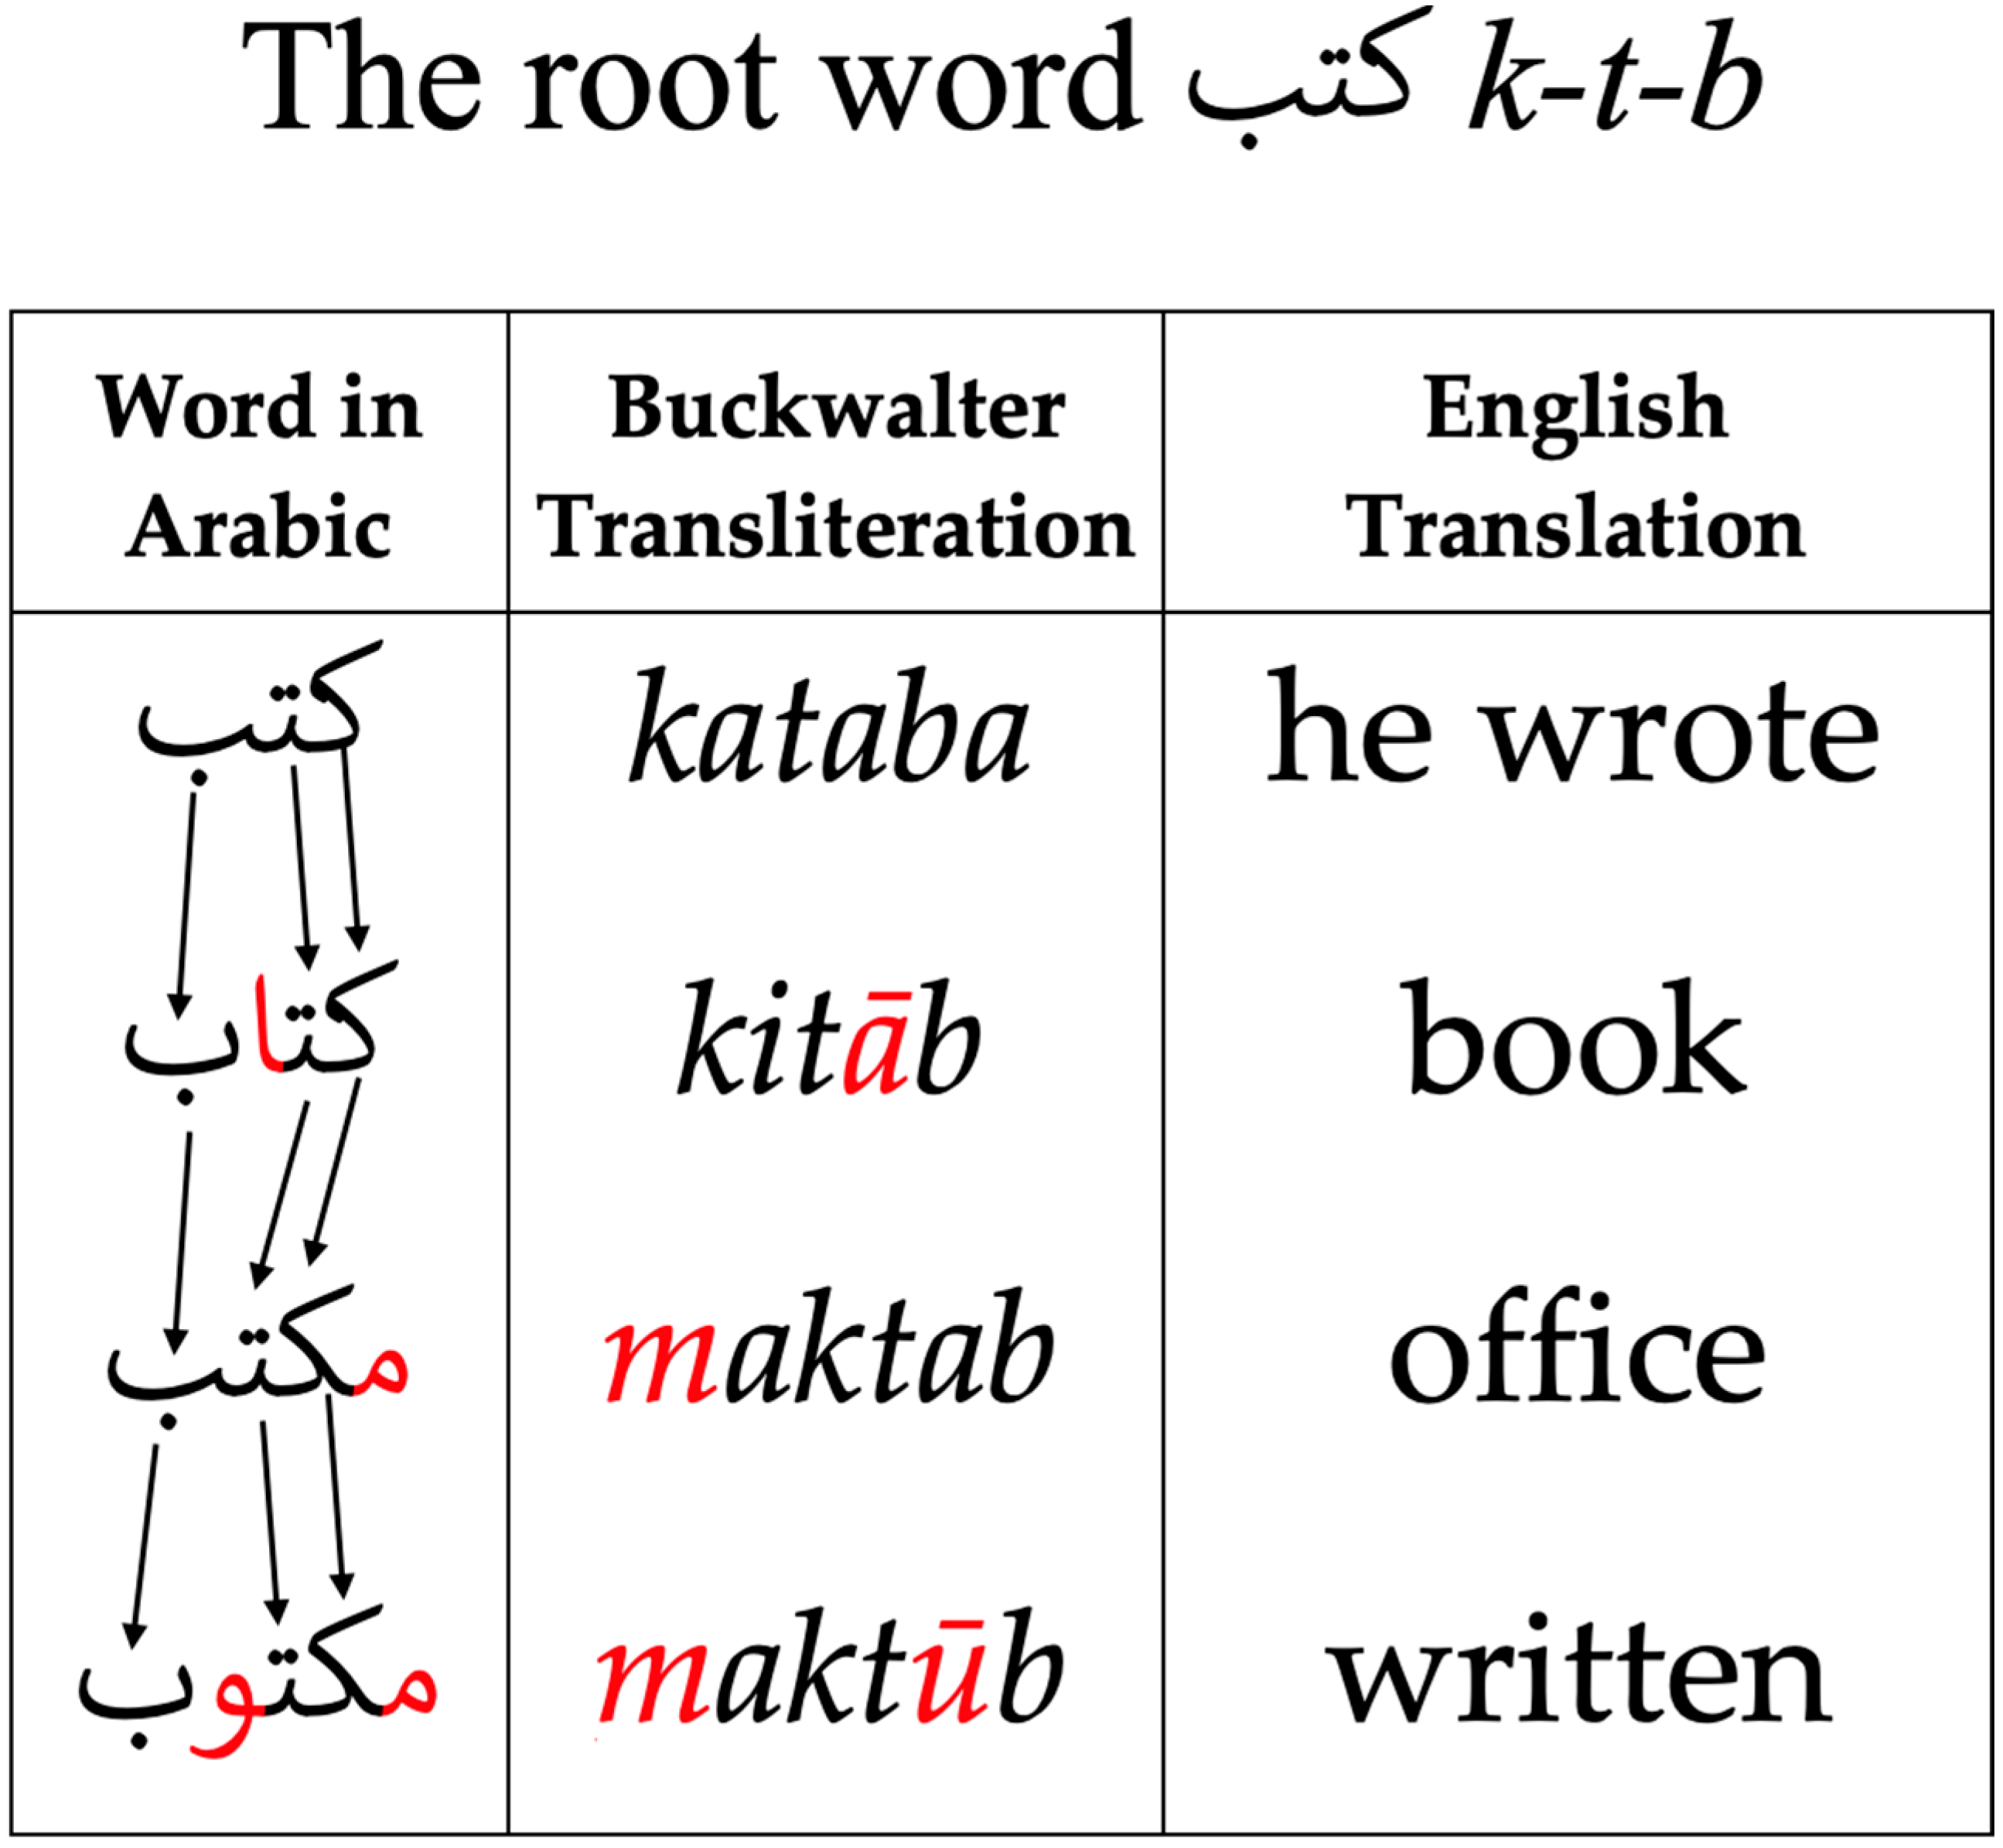
\includegraphics[width=0.72\textwidth]{morphology.png}

\caption{Example of Arabic morphological derivation from the root ``k-t-b'', illustrating the richness and complexity of Arabic word formation.}

\label{fig:arabic_morphology}

\end{figure}

\vspace{0.3cm}

In addition to root-based derivation, Arabic exhibits extensive \emph{cliticization}: function words such as the definite article, conjunctions, prepositions and pronouns are written attached to a host word. For example, the single written token\textit{walfid\d{d}a} (meaning and the silver) joins three morphological units: the conjunction\textit{wa+} (meaning *and*), the definite article\textit{al+} (``the''), and the noun \textit{fid\d{d}a} (``silver''). The The BAREC annotation guidelines explicitly name the presence and type of clitics as markers of readability level \cite{habash2025guidelines},which is why making them explicit through morphological segmentation (D3Tok) is central to the methodology of this thesis.

Lexical ambiguity is another important challenge, since a single undiacritized Arabic word can correspond to several distinct readings. For example, the word \textit{`ilm}/\textit{`alam}/\textit{`allama} can mean \emph{knowledge}, \emph{flag} or \emph{he taught} depending on the context. Ambiguity has a direct effect on readability, because resolving the rarer readings requires more advanced linguistic knowledge, and the BAREC guidelines therefore place constructions that need diacritization for disambiguation at the higher readability levels. Arabic syntax also allows flexible word order, which makes sentences harder for machine learning models to understand.

Compared with English readability research, Arabic readability assessment also has few large scale annotated datasets and benchmark resources. The BAREC dataset improved this situation considerably, but fine grained readability prediction across 19 ordered levels is still a difficult task.

These challenges lead to two complementary design decisions. First, we use pretrained transformer models, whose contextual representations learned from large Arabic corpora help with the morphological, lexical and syntactic complexity. Second, we use ordinal aware learning methods to model the ordered structure of the readability levels, which standard classification ignores.
\section{Problem Statement}
Traditional readability assessment systems often treat readability prediction as a standard classification problem trained with Cross Entropy loss. Readability levels, however, are ordered by nature, and nearby levels are more similar than distant ones.

In standard classification, when the true level is 11, predicting level 10 gets exactly the same penalty as predicting level 1, although the first is a near miss and the second a far miss. Because of this, classification models cannot properly capture the ordinal structure of readability labels.

This thesis therefore investigates the following question: given a fixed AraBERTv2 backbone with D3Tok morphological segmentation and the training protocol of the BAREC benchmark, \emph{which ordinal head and loss function achieves the highest Quadratic Weighted Kappa (QWK) among cross entropy, regression with mean squared error, ordinal log loss, an Earth Mover's Distance loss, four soft label settings, a CORAL ordinal head and a Soft QWK schedule in two phases; how do the loss families differ in the trade off between exact match accuracy and distance aware agreement; and are their errors near misses or far misses?}


\subsection{Research Objectives}
The main objectives of this thesis are:
\begin{itemize}

\item Determine which ordinal head and loss function give the highest QWK on the BAREC benchmark when the corpus, the encoder and the entire training protocol stay fixed.
\item Compare nine head and loss configurations on a single AraBERTv2 and D3Tok backbone, and report the two-phase Soft-QWK schedule beside them as a separate group.

\item Quantify the trade off between exact-match accuracy (\textit{Acc19}) and distance aware agreement (QWK) across the loss families.

\item Measure the error distance of each method, separating near misses from far misses, as the research topic requires.

\item Establish whether a CORAL head can learn its cut points under this protocol at all, and what its cut points should be initialised to if it cannot.

\item Measure how much of the difference between published systems is due to the checkpoint selection rule and the decision threshold rather than to the loss.

\item Evaluate predictions at multiple granularities ($19$, $7$, $5$ and $3$ levels) using the BAREC collapsing scheme.

\item Compare the results with the original BAREC benchmark, with the systems of the BAREC 2025 Shared Task and with the agreement between human annotators.

\end{itemize}



\subsection{Research Contributions}
The main contributions of this thesis are:

\begin{itemize}

\item A controlled comparison of nine head and loss configurations on one fixed pipeline, which extends the four losses of the BAREC benchmark with a CORAL ordinal head, four soft-label settings and a metric-aligned two-phase objective, and reports them in a single table on both official splits.
Compare the results with the original BAREC benchmark, with the systems of the BAREC 2025 Shared Task and with the agreement between human annotators.
\item A verified reproduction of the benchmark's loss comparison, where the one visible discrepancy is explained and traced back to the checkpoint selection rule.

\item An initialisation of the CORAL cut points from the cumulative training label frequencies, motivated by how far the benchmark learning rate lets them travel. We pair it with a direct measurement of how much the cut points actually move and with two ablations that test the argument from opposite directions.
\item Two metrics of error distance, the share of predictions at least three and at least five levels away from the gold level. They separate near misses from far misses and show that the lead in QWK comes from removing far misses and not from lowering the average error.

\item A measurement of how much the checkpoint selection rule and the CORAL decision threshold are worth, which is what makes systems published under different protocols comparable.

\item A track with a frozen backbone that satisfies the CPU friendly requirement of the research topic, reports variance over five seeds and shows that the ranking of the losses on frozen features does not carry over to fine tuning.

\item A comparison of the results with the published BAREC benchmark, the systems of the BAREC 2025 Shared Task and the reported agreement between human annotators.

\end{itemize}

\subsection{Methodology Overview}
The proposed system for Arabic readability assessment combines a pretrained transformer language model with ordinal aware learning methods. The overall pipeline is shown in Figure~\ref{fig:pipeline} and proceeds as follows.

The pipeline begins with the BAREC corpus, where each Arabic sentence carries an ordered readability level from 1 to 19. The input is the D3Tok column of the corpus, a morphologically segmented form in which clitics are separated from their host word and marked with a \texttt{+}. That representation is used because AraBERTv2 was pretrained on morphologically segmented Arabic, so segmented input matches its pretraining distribution, and because the pairing of AraBERTv2 with D3Tok input is the configuration the original benchmark carries into its loss comparison \cite{elmadani2025barec}.The segmented text is tokenised and passed to AraBERTv2, and after dropout the pooled output of the encoder, a vector of 768 dimensions, is used as the sentence representation.

This representation goes to a prediction head whose form depends on the configuration. The softmax losses (cross entropy, ordinal log loss, EMD and the four soft label settings) use a linear layer with 19 outputs, regression and the Soft QWK schedule use a linear layer with a single output, and CORAL uses a layer with 18 thresholds and one shared projection. During training, the corresponding loss compares the output of the head with the gold label. At inference, the output is decoded to a level between 1 and 19 by taking the highest score, by rounding, or by counting how many thresholds are exceeded. Every configuration is trained and evaluated under the same protocol, with QWK as the primary metric, together with exact accuracy (\textit{Acc19}), adjacent accuracy ($\pm 1$ \textit{Acc19}), average distance (\textit{Dist}), the collapsed $7$-, $5$- and $3$-level accuracies, and the two error-distance metrics introduced in this thesis.
\begin{figure}[H]
    \centering
    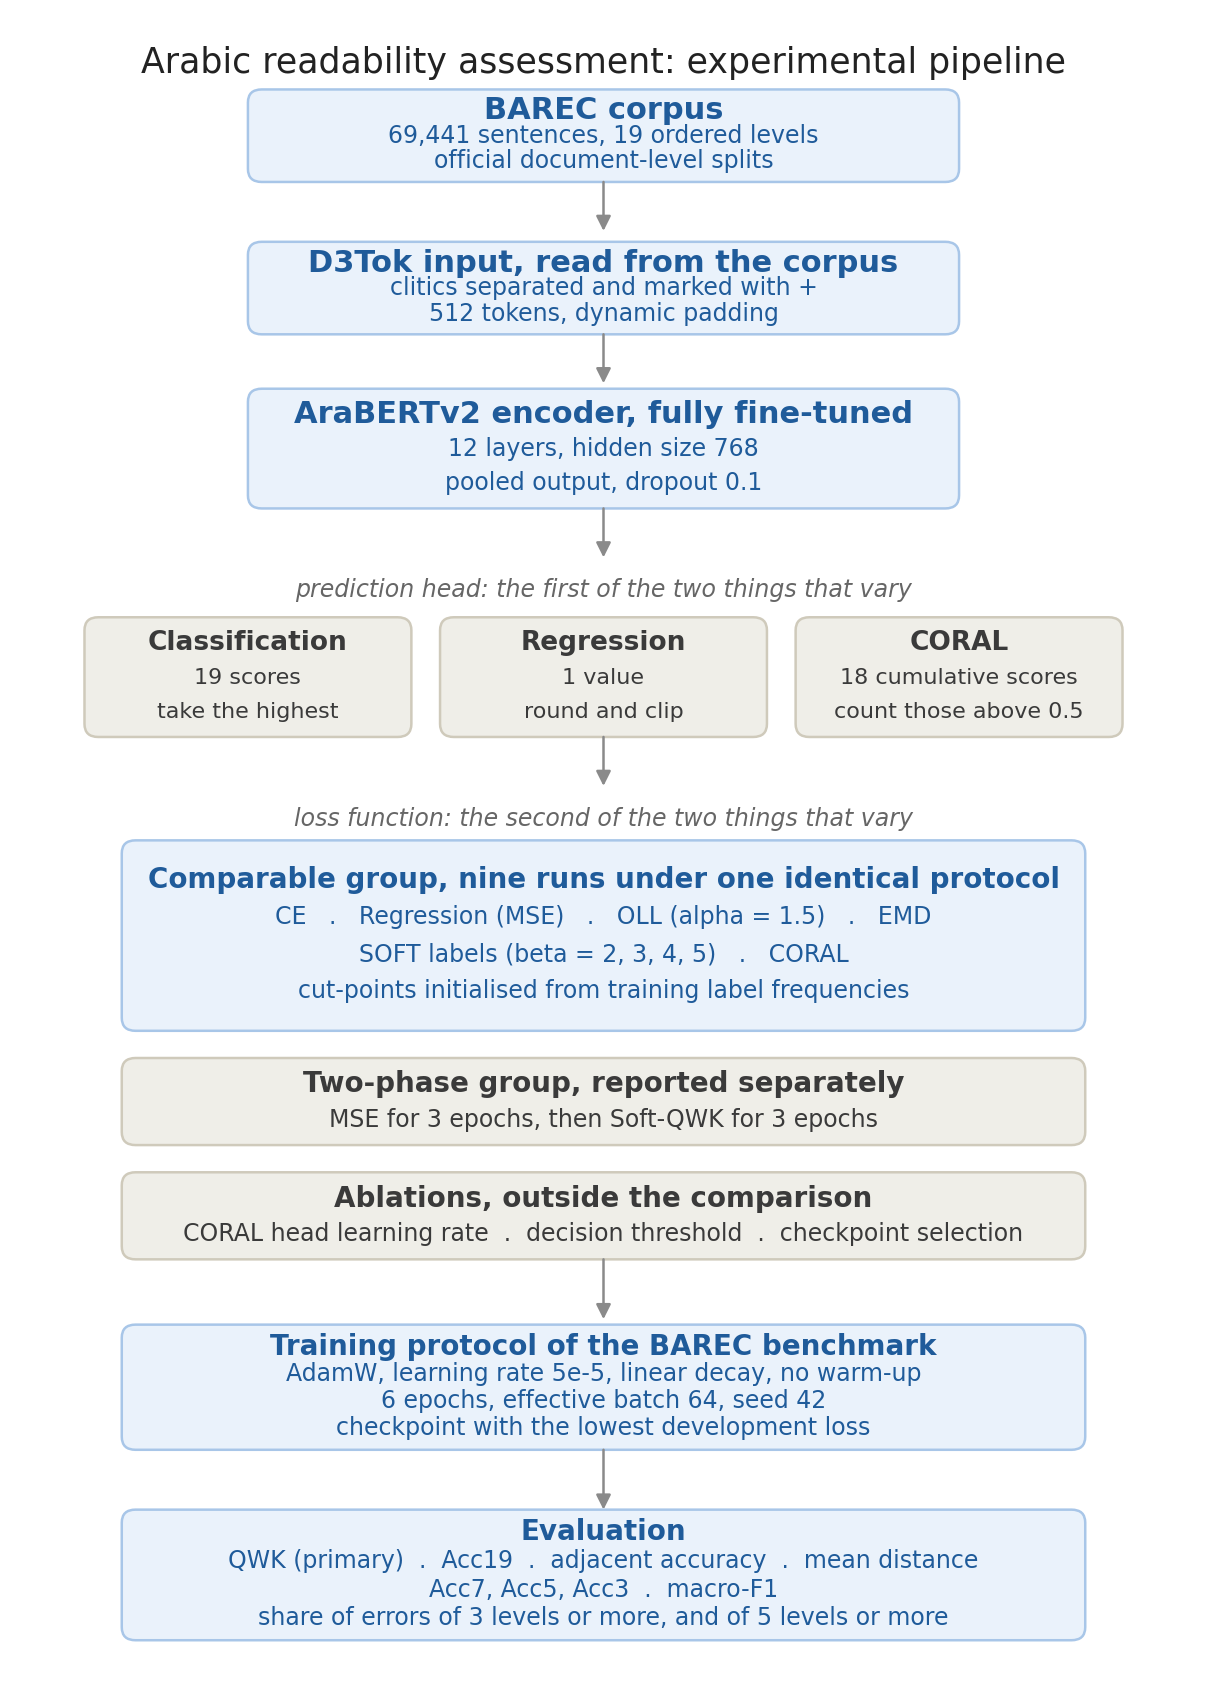
\includegraphics[width=0.78\linewidth]{pipeline.png}
    \caption{The experimental pipeline. Everything drawn in blue is held fixed for every run; the prediction head and the loss function, drawn in grey, are the only components that vary.}
    \label{fig:pipeline}
\end{figure}
\vspace{0.3cm}


\subsection{Thesis Organization}

This thesis is organized as follows:

\vspace{0.3cm}

\begin{itemize}

\item \textbf{Chapter 1 -- Introduction:}
This chapter introduces the background and motivation of Arabic readability assessment. It also presents the research objectives, the challenges, the contributions, an overview of the methodology and the evaluation metrics used in this work.

\vspace{0.2cm}

\item \textbf{Chapter 2 -- Related Work:}
This chapter reviews previous studies related to Arabic readability assessment, Arabic NLP challenges, pretrained language models, ordinal regression methods, and systems developed using the BAREC dataset.

\vspace{0.2cm}

\item \textbf{Chapter 3 -- Proposed Methodology:}
This chapter describes the corpus and its splits, the D3Tok input representation, the encoder and the three prediction heads, and the exact form of every loss function with the tests that verify it. It then covers the initialisation of the CORAL cut points, the training protocol with every declared difference from the published script, the evaluation metrics and the track with a frozen backbone.
\vspace{0.2cm}

\item \textbf{Chapter 4 -- Experiments and Results:}
This chapter reports the integrity checks, the reproduction of the published benchmark and the full results of the eleven runs on both splits. It then examines the trade off between exact accuracy and ordinal agreement, the analysis of error distance, the four ablations and the track with a frozen backbone, and ends with a comparison against published systems and human agreement, followed by the limitations.

One thing to check: this section says four ablations, but the abstract says three.
\vspace{0.2cm}

\item \textbf{Chapter 5 -- Conclusion and Future Work:}
The final chapter brings the findings together, states the contributions and the limitations, and sets out the next steps. The first of these is a study over multiple seeds, which would turn the leading group from an observation into a measurement.
\end{itemize}


\section{Summary of Introduction}
This chapter introduced the context of Arabic readability assessment and the challenges that make it harder than English readability, namely morphological richness, lexical ambiguity and syntactic complexity. It then stated the research question, which asks which ordinal head and loss function gives the highest QWK on BAREC when the protocol is held fixed, and whether the errors are near misses or far misses. It also listed the nine configurations of the comparable group, the Soft QWK schedule in two phases reported next to them, and the ablations. The methodology overview described the AraBERTv2 and D3Tok pipeline and the evaluation metrics.
\textit{The next chapter reviews previous work on readability assessment, pretrained language models, the BAREC corpus, ordinal regression methods and the systems built for the BAREC 2025 Shared Task.}
% Chapter 2: 
\chapter{Literature Review}
\label{chap:relatedwork}
\section{Introduction}

This chapter reviews previous studies on readability assessment, Arabic Natural Language Processing, pretrained transformer language models and ordinal regression methods. It follows how readability prediction moved from traditional handcrafted formulas to modern deep learning and transformer based architectures.

The chapter also presents the challenges of Arabic readability, the existing Arabic readability datasets and earlier work built on pretrained language models such as AraBERTv2. It then reviews the ordinal classification and distance aware learning approaches that motivate the methodology of this thesis. Finally, it surveys the systems developed for the BAREC 2025 Shared Task, since they are the most directly comparable prior work.

\section{Readability Assessment}

\subsection{Traditional Readability Formulas}

Early readability assessment research relied mainly on handcrafted statistical formulas designed to estimate text difficulty using shallow linguistic features such as sentence length, word length, and syllable count \cite{dubay2004principles}.
The Flesch Reading Ease (FRE), the Flesch Kincaid Grade Level (FKGL), the SMOG index and the Gunning Fog index are among the most widely used traditional readability formulas. They were first developed for English texts and became popular because they are simple and cheap to compute.

These formulas assume that longer sentences and more complex words mean a text is harder to read. They give fast estimates, but they miss the deeper semantic, syntactic and contextual information that accurate readability prediction needs.

\begin{table}[H]

\centering

\caption{Examples of traditional readability formulas.}

\label{tab:traditional_readability}

\begin{tabular}{p{4cm} p{6cm} p{2.5cm}}

\toprule

\textbf{Formula} & \textbf{Main Features} & \textbf{Language} \\

\midrule

Flesch Reading Ease (FRE) & Sentence length and word length & English \\

Flesch-Kincaid Grade Level (FKGL) & Sentence length and syllable count & English \\

SMOG Index & Number of complex words & English \\

Gunning Fog Index & Sentence complexity and word difficulty & English \\

\bottomrule

\end{tabular}

\end{table}



\begin{figure}[H]
    \centering
    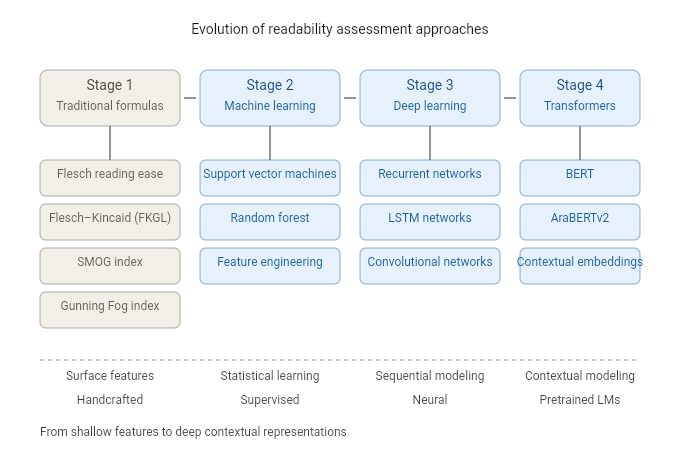
\includegraphics[width=0.98\linewidth]{readability_assessment_evolution@1x.png}
    \caption{How readability assessment evolved, from traditional handcrafted formulas to modern contextual language models based on transformers.}
    \label{fig:evolution}
\end{figure}

\vspace{0.3cm}


Traditional readability formulas are simple and cheap to compute, but they have several important limitations. They rely mostly on shallow handcrafted features and miss semantic meaning, contextual dependencies and linguistic information at the discourse level. These limitations matter even more for morphologically rich languages such as Arabic, where lexical ambiguity and complex word formation patterns make readability prediction considerably harder\cite{habash2010introduction}.

As research on readability assessment moved forward, machine learning approaches appeared as more powerful alternatives that learn complex linguistic patterns automatically from data. Where traditional handcrafted formulas use a fixed set of shallow features, machine learning methods can exploit a much larger set of lexical, syntactic and statistical features and predict readability more accurately.
\subsection{Machine Learning Approaches}

Machine learning approaches improved considerably on traditional readability formulas, because they learn from data instead of relying only on fixed handcrafted rules. They usually treat readability assessment as a supervised classification or regression problem over manually extracted linguistic features.

Early machine learning systems for readability commonly used lexical, syntactic and statistical features such as sentence length, word frequency, the distribution of parts of speech, the depth of the parse tree and probabilities from language models \cite{schwarm2005reading}.

Several traditional machine learning algorithms have been widely used for readability prediction, including Support Vector Machines (SVM), Random Forests, Logistic Regression, and Naive Bayes classifiers. These models demonstrated improved flexibility and predictive performance compared to traditional readability formulas.

\begin{table}[H]

\centering

\caption{Common machine learning methods used for readability assessment.}

\label{tab:ml_readability}

\begin{tabular}{p{4cm} p{7cm} p{2.5cm}}

\toprule

\textbf{Method} & \textbf{Main Characteristics} & \textbf{Learning Type} \\

\midrule

Support Vector Machines (SVM) & Margin-based supervised classification & Supervised \\

Random Forest & Ensemble decision tree learning & Supervised \\

Logistic Regression & Linear probabilistic classification & Supervised \\

Naive Bayes & Probabilistic feature-based classification & Supervised \\

\bottomrule

\end{tabular}

\end{table}
Notably, the original BAREC benchmark also reports SVM and Decision Tree baselines for Arabic readability: an SVM with a count vectorizer on D3Tok input reaches a QWK of only 56.5\%, and a Decision Tree reaches 52.5\% \cite{elmadani2025barec}.These results confirm that non neural methods are not sufficient for fine grained Arabic readability prediction over 19 levels.
\subsection{Deep Learning Approaches}

Deep learning approaches advanced readability assessment considerably, because they learn hierarchical features automatically from raw text. Traditional machine learning systems depend heavily on handcrafted linguistic features, whereas deep neural networks learn semantic and contextual representations by themselves from large corpora.

Several deep learning architectures have been applied to readability prediction, among them Recurrent Neural Networks (RNN), Long Short Term Memory networks (LSTM) and Convolutional Neural Networks (CNN). These models perform better because they capture sequential dependencies and semantic relations inside the text \cite{martinc2021supervised}.

Recurrent Neural Networks are especially effective at modeling sequential textual information, and LSTM networks learn long range dependencies better thanks to their memory mechanisms. Convolutional Neural Networks have also been applied successfully to readability assessment, where they extract local semantic and syntactic patterns from text representations.

\begin{table}[H]

\centering

\caption{Common deep learning architectures used for readability assessment.}

\label{tab:deep_learning_readability}

\begin{tabular}{p{4cm} p{7cm} p{2.5cm}}

\toprule

\textbf{Architecture} & \textbf{Main Characteristics} & \textbf{Learning Type} \\

\midrule

RNN & Sequential text modeling & Deep Learning \\

LSTM & Long-range dependency modeling & Deep Learning \\

CNN & Local feature extraction and pattern learning & Deep Learning \\

BiLSTM & Bidirectional contextual sequence modeling & Deep Learning \\

\bottomrule

\end{tabular}

\end{table}

Deep learning approaches improved substantially on traditional machine learning methods, but these architectures still had trouble capturing long range contextual dependencies efficiently. Training deep neural networks from scratch also requires large annotated datasets and considerable computational resources.

Transformer based pretrained language models then changed Natural Language Processing, since their self attention mechanisms and their pretraining on large corpora allow them to understand language in context.

\subsection{Transformer-Based Language Models}

Transformer based language models were a major advance in Natural Language Processing, because their self attention mechanisms let them understand language efficiently in context \cite{vaswani2017attention}. Where recurrent neural networks process a sequence step by step, transformer architectures process it in parallel, which lets them model long range dependencies and contextual relations between words more effectively.

One of the most influential transformer models is Bidirectional Encoder Representations from Transformers (BERT), which learns context in both directions to produce deep semantic representations of text \cite{devlin2019bert}.BERT is pretrained on very large text corpora with self supervised objectives such as masked language modeling and next sentence prediction.

Transformer based pretrained language models improved performance considerably on many NLP tasks, among them text classification, sentiment analysis, machine translation, question answering and readability assessment. They capture complex semantic, syntactic and contextual information better than earlier machine learning and deep learning approaches.
\begin{table}[H]

\centering

\caption{Examples of transformer-based language models used in NLP.}

\label{tab:transformer_models}

\begin{tabular}{p{4cm} p{6.5cm} p{2.5cm}}

\toprule

\textbf{Model} & \textbf{Main Characteristics} & \textbf{Language} \\

\midrule

BERT & Bidirectional contextual transformer model & English \\

RoBERTa & Optimized robust BERT pretraining & English \\

DistilBERT & Lightweight compressed transformer model & English \\

AraBERTv2 & Transformer model optimized for Arabic NLP & Arabic \\

\bottomrule

\end{tabular}

\end{table}
Among transformer models, Arabic pretrained language models have attracted growing attention because of the particular linguistic complexity of Arabic. Several Arabic transformer architectures have been proposed to improve Arabic language understanding, and AraBERTv2 performs strongly across many Arabic NLP tasks.

\subsection{AraBERTv2 for Arabic NLP}

AraBERTv2 is a pretrained transformer language model designed specifically for Arabic Natural Language Processing tasks\cite{antoun2020arabert}.The model uses the BERT architecture (12 layers, 12 attention heads, hidden representations of 768 dimensions) and was pretrained on about 8.6 billion words of Arabic text taken from news articles, Wikipedia and other sources.

What sets AraBERTv2 apart, and the reason we choose it as the backbone in this thesis, is the preprocessing used during pretraining. The original AraBERT was pretrained on plain Arabic text at the word level, while AraBERTv2 was pretrained on text that had first been segmented morphologically with the Farasa segmenter\cite{darwish2016farasa}. Farasa splits clitics from their host words and marks the boundaries with a "+" character, which is the same segmentation principle as the D3Tok input representation. When AraBERTv2 receives D3Tok input, the segmented tokens therefore match the distribution it saw during pretraining.

The original BAREC benchmark confirms how much this match matters. Among the four Arabic models tested (AraBERTv02, AraBERTv2, MARBERTv2 and CamelBERT msa), AraBERTv2 was the \emph{only} one whose performance improved with D3Tok input, rising from 76.3\% to 80.0\% QWK on the development set, while the other three models performed the same or worse with D3Tok compared to plain word input \cite{elmadani2025barec}. This empirical result justifies the choice of AraBERTv2 as the fixed backbone in the present work.

\begin{figure}[H]
    \centering
    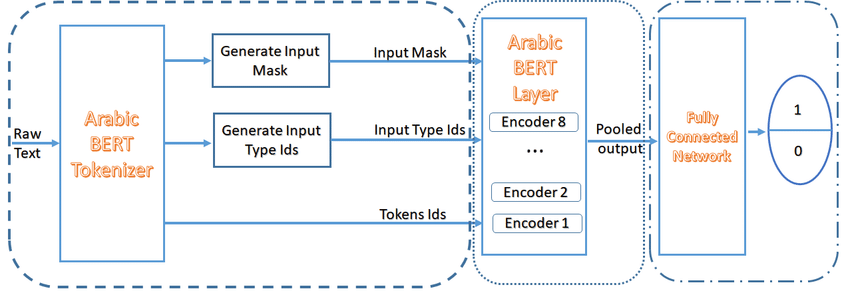
\includegraphics[width=0.79\linewidth]{Arabic-BERT-model-architecture.png}
    \caption{General architecture of transformer-based Arabic language models such as AraBERTv2 for contextual language understanding.}
    \label{fig:arabert_arch}
\end{figure}

\vspace{0.3cm}

Figure~\ref{fig:arabert_arch} shows the general architecture of transformer based Arabic language models. Through its contextual embeddings and self attention mechanisms, AraBERTv2 models the semantic and syntactic relations between Arabic words more effectively than traditional machine learning and earlier deep learning approaches. In readability prediction these contextual representations have a clear advantage over handcrafted features, since they model the semantic complexity and the linguistic dependencies inside the text in more depth.


In readability prediction, the contextual representations of transformer models have a clear advantage over traditional handcrafted features, since they model the semantic complexity and the linguistic dependencies inside the text in more depth.
\subsection{Arabic Readability Datasets}

Building and evaluating automatic readability assessment systems requires annotated datasets of good quality. Compared with English readability research, Arabic readability assessment still has few publicly available benchmark datasets and annotated corpora\cite{nassiri2023approaches}.

Several Arabic readability datasets and resources have appeared in recent years. The SAMER project produced a leveled readability lexicon for Standard Arabic with a scale of five levels covering 40,687 lemma and POS pairs \cite{alkhalil2020samer}, which later served as the basis for the SAMER corpus for Arabic text simplification \cite{alhafni2024samer}. DARES provided a readability assessment dataset collected from Saudi school materials \cite{elhaj2024dares}. The OSMAN metric adapted readability scoring to Arabic by taking script specific markers and diacritization into account \cite{elhaj2016osman}. ReadMe++ introduced a multilingual readability benchmark over several domains, whose Arabic split is relevant to Arabic readability research \cite{naous2024readme}. Liberato et al.\ explored strategies for Arabic readability modeling using pretrained models on the SAMER corpus \cite{liberato2024strategies}.

Despite this progress, most existing Arabic readability datasets use coarse scales of only 3 to 5 levels, which limits how finely a model can learn to distinguish between them. This limitation led to a larger and more complete resource, the Balanced Arabic Readability Evaluation Corpus (BAREC), which supports fine grained ordinal readability assessment over 19 ordered levels \cite{elmadani2025barec}.

\subsection{The BAREC Dataset}

The Balanced Arabic Readability Evaluation Corpus (BAREC) was introduced as a large scale benchmark dataset for Arabic readability assessment \cite{elmadani2025barec}. The corpus contains 69,441 Arabic sentences spanning more than one million words, collected from 1,922 documents across three domains (Arts \& Humanities, Social Sciences, and STEM) and three readership groups (Foundational, Advanced, and Specialized).

The main strength of BAREC is its fine grained annotation scheme of 19 ordered readability levels, which follow the Abjad order of the Arabic letters (1-\textit{alif} through 19-\textit{qaf}) and run from kindergarten to postgraduate comprehension. Through the BAREC pyramid the 19 levels can be collapsed into coarser schemes of 7, 5 and 3 levels, so a single model trained at the finest granularity can be evaluated at any coarser one. Six expert Arabic educators annotated the corpus manually, following an adaptation of the Taha Thomure leveling guidelines, and a separate paper describes the annotation protocol in detail \cite{habash2025guidelines}. The reported average pairwise inter-annotator agreement, measured by QWK, is 81.8\%, indicating substantial agreement. The dataset is split at the document level into training (80\%), development (10\%), and test (10\%) sets to prevent data leakage.

\begin{table}[H]

\centering

\caption{Main characteristics of the BAREC dataset.}

\label{tab:barec_characteristics}

\begin{tabular}{p{5cm} p{6cm}}

\toprule

\textbf{Characteristic} & \textbf{Description} \\

\midrule

Language & Modern Standard Arabic \\

Number of Sentences & 69,441 (over 1M words) \\

Documents / Domains & 1,922 documents; 3 domains \\

Readability Levels & 19 ordered levels (collapsible to 7/5/3) \\

Annotation & Manual, by 6 expert Arabic educators \\

Inter-Annotator Agreement & 81.8\% pairwise QWK \\

Target Levels & Kindergarten to postgraduate \\

Data Split & 80\% train / 10\% dev / 10\% test (document-level) \\

\bottomrule

\end{tabular}

\end{table}

The fine grained ordinal structure of BAREC makes it well suited to evaluating ordinal aware learning approaches. Readability levels are ordered by nature, so a prediction error between nearby levels should be penalized less than one between distant levels. The original BAREC benchmark gives the reference results: the best single model (AraBERTv2 + D3Tok + Regression) reaches a test set QWK  of 84.4\%, an average ensemble of six models reaches 84.5\%, and an oracle upper bound that selects the best prediction per sentence reaches 94.7\% \cite{elmadani2025barec}. These figures frame the difficulty of the task and provide the comparison points used in Chapter~4.
\subsection{Ordinal Regression and Distance-Aware Learning}

Ordinal regression is a machine learning paradigm made for prediction tasks whose labels have a natural order \cite{gutierrez2016ordinal}.Where traditional classification treats the classes as unrelated, ordinal prediction takes the relative distance between them into account, which makes it well suited to readability assessment.

In readability prediction the levels are ordered by nature. Predicting level 10 instead of level 11 should count as a smaller error than predicting level 10 instead of level 1. Traditional classification approaches trained with Cross Entropy loss do not model such ordinal relations between labels explicitly.

Several ordinal aware learning methods have been proposed in the literature to address this limitation. They add the ordering of the labels to the training process and penalize distant prediction errors more heavily than nearby ones.
\begin{table}[H]

\centering

\caption{Common ordinal-aware learning methods used for readability assessment.}

\label{tab:ordinal_methods}

\begin{tabular}{p{3.2cm} p{6.5cm} p{3cm}}

\toprule

\textbf{Method} & \textbf{Main Characteristics} & \textbf{Learning Paradigm} \\

\midrule

Cross-Entropy (CE) & Standard classification without ordinal awareness & Classification \\

Regression (MSE) & Continuous ordinal prediction via squared-error loss & Regression \\

CORAL & Ordered binary classifiers ($K{-}1$ cumulative thresholds) & Ordinal Regression \\

Ordinal Log Loss (OLL) & Distance-weighted cross-entropy penalization & Ordinal Regression \\

Earth Mover's Distance (EMD) & Cumulative-distribution (transport-cost) optimization & Ordinal Regression \\

Soft-QWK & Differentiable surrogate of the QWK evaluation metric & Ordinal Regression \\

\bottomrule

\end{tabular}

\end{table}

Among ordinal-aware approaches, CORAL models ordinal prediction through a sequence of $K{-}1$ ordered binary classification tasks, so that the ordering is encoded in the output structure \cite{cao2020coral}. Ordinal log loss extends cross-entropy by weighting the probability given to each wrong level by its distance from the true level \cite{castagnos2022ordinal}. The soft-label loss replaces the one-hot target by a target that decays with distance \cite{bertinetto2020soft}, and the Earth Mover's Distance loss penalises the difference between the predicted and target cumulative distributions \cite{hou2017emd}. The Soft-QWK loss optimises a differentiable surrogate of the QWK metric \cite{delatorre2018wkl,diaz2019softlabels}; because that surrogate is a statistic of the whole batch, it can be lowered by predicting near the mean level, and the STBW system therefore precedes it with a mean squared error warm-up phase \cite{trigui2025stbw}, a design this thesis follows and evaluates in Chapter~\ref{chap:results}.

These methods have demonstrated promising improvements for ordinal prediction tasks across several domains, including medical diagnosis, age estimation, educational assessment, and readability prediction \cite{castagnos2022ordinal}.
\section{Systems Developed for the BAREC Shared Task}

The release of the BAREC corpus came with the BAREC 2025 Shared Task on Arabic readability assessment, organized at the Third Arabic Natural Language Processing Conference (ArabicNLP 2025) \cite{elmadani2025sharedtask}. The shared task attracted 22 registered teams from 12 countries, and 17 of them submitted system description papers. It defined two sub tasks, at sentence level and at document level, and three resource tracks, Strict, Constrained and Open, with QWK on a blind test set as the official ranking metric.

The most successful systems combined morphological segmentation (D3Tok) with Arabic pretrained language models, ordinal aware losses and ensembling. Large language models and less standard architectures such as graph neural networks and vision language models generally did worse than the transformer baselines. Only five teams went above the strongest baseline of the organizers (AraBERTv2 + D3Tok + Regression, 84.6\% blind QWK).

Two systems are especially relevant to this thesis. The ZAI system used AraBERTv2 with a CORAL ordinal regression head, trained with a binary cross entropy summed over the $K{-}1$ cumulative thresholds. It selected the checkpoint by QWK, stopped early with a patience of two epochs, and used a single decision threshold tuned on the development set; it reached 85.5\% QWK on the blind test set \cite{nazzal2025zai}.The STBW system used AraBERTv2 with a regression head of a single neuron and a schedule in two phases, a warm up with mean squared error followed by a differentiable Soft QWK objective, which raised its own test QWK from 83.9\% to 84.88\% and reached 85.6\% on the blind test set. Besides the segmented sentence, its input also carries corpus metadata and surface statistics \cite{trigui2025stbw}. These two systems are the reason we include both CORAL and Soft QWK in the present comparison. Their protocols differ, so this thesis reimplements both mechanisms inside one fixed pipeline instead of comparing published numbers.

Table~\ref{tab:barec_systems} ssummarizes the corpus benchmark, the baselines of the organizers and the participating systems of the shared task, together with their approaches and their QWK scores at sentence level.\footnote{Two systems (ZAI and ANLPers) trained on the development set and are marked with an asterisk; their scores are not strictly comparable.}

\begin{table}[H]
\centering
\footnotesize
\caption{Work on the BAREC dataset: corpus benchmark, organizer baselines, and BAREC 2025 Shared Task systems (sentence-level, Strict track). QWK is the primary metric; higher is better.}
\label{tab:barec_systems}
\begin{tabular}{p{2.4cm} p{0.8cm} p{4.8cm} p{2.2cm} p{1.2cm}}
\toprule
\textbf{Team / Source} & \textbf{Year} & \textbf{Model / Approach} & \textbf{Loss / Method} & \textbf{QWK (\%)} \\
\midrule
\multicolumn{5}{l}{\textit{Corpus benchmark (Elmadani et al., 2025) --- test set}} \\
\midrule
BAREC best single & 2025 & AraBERTv2 + D3Tok & Regression (MSE) & 84.4 \\
BAREC ensemble & 2025 & Average of 6 AraBERTv2 models & Ensemble & 84.5 \\
BAREC oracle & 2025 & Best-of-6 per sentence & Oracle & 94.7 \\
SVM baseline & 2025 & SVM, count vectorizer, D3Tok & Classification & 56.5 \\
\midrule
\multicolumn{5}{l}{\textit{Organizer baselines --- blind test set}} \\
\midrule
Baseline III & 2025 & AraBERTv2 + D3Tok & Regression & 84.6 \\
Baseline II & 2025 & AraBERTv2 + D3Tok & CE & 81.5 \\
Baseline I & 2025 & AraBERTv02 + Word & CE & 80.5 \\
\midrule
\multicolumn{5}{l}{\textit{Shared Task systems --- blind test set (Strict track, sentence-level)}} \\
\midrule
!MSA & 2025 & Ensemble of 4 Arabic PLMs + LLM augmentation & CE + OLL + MSE + ordinal & \textbf{87.5} \\
AMAR & 2025 & Stacked meta-learner over 7 transformers & Regression + meta-classifier & 86.4 \\
mucAI & 2025 & AraBERTv2 + conformal prediction & CE / EMD / Focal & 85.7 \\
STBW & 2025 & AraBERTv2, two-phase training & MSE $\rightarrow$ Soft-QWK & 85.6 \\
ZAI & 2025 & AraBERTv2 + CORAL ordinal head & CORAL (BCE) & 85.5* \\
Syntaxa & 2025 & AraBERTv2 + dependency-graph GNN & GNN & 84.3 \\
MorphoArabia & 2025 & Morphology-aware regression & Regression & 84.2 \\
MARSAD & 2025 & Specialized AraBERT, two-stage & CE $\rightarrow$ WKL & 84.1 \\
Noor & 2025 & Hybrid transformer + features & PLM + features & 83.1 \\
Phantoms & 2025 & Hybrid BERT + linguistic features & PLM + features & 82.7 \\
Qais & 2025 & Fine-tuned PLM (+ LLM) & Classification & 82.5 \\
LIS & 2025 & Curriculum learning with PLMs & Curriculum & 82.4 \\
SATLab & 2025 & Character/token $n$-grams (non-neural) & ML & 82.3 \\
PalNLP & 2025 & Ordinal regression + $K$-fold ensemble & Ordinal regression & 81.1 \\
GNNinjas & 2025 & Lexicon-enriched graph modeling & GNN & 78.5 \\
ANLPers & 2025 & Neural classifiers on embeddings & Neural classifier & 73.0* \\
Pixel & 2025 & Vision-language rendered-text model & VLM & 66.2 \\
\bottomrule
\end{tabular}

\vspace{0.15cm}
{\footnotesize * Trained on the development set; not strictly comparable to the other systems.}
\end{table}

This thesis has a different objective from the shared task systems. It does not try to maximise leaderboard performance through ensembling, data augmentation or external resources. It isolates the effect of the ordinal head and the loss function on a single fixed AraBERTv2 and D3Tok backbone, with every other component kept at the value the benchmark script sets, which gives a controlled view of how much each ordinal aware mechanism contributes on its own.

\section{Summary}

This chapter reviewed the main lines of research on readability assessment, Arabic Natural Language Processing, transformer based language models and ordinal aware learning methods.

It presented the traditional readability formulas with their limitations, including the OSMAN metric designed for Arabic, then discussed machine learning and deep learning approaches as more advanced alternatives. It then reviewed transformer based pretrained language models, with particular attention to AraBERTv2, and explained why its pretraining on Farasa segmented text makes it the right backbone for D3Tok input.

The chapter also surveyed the existing Arabic readability datasets, among them the SAMER lexicon, DARES, OSMAN and ReadMe++, and focused on the BAREC corpus as a large scale benchmark for fine grained ordinal readability assessment, with its published benchmark results. Ordinal regression and distance aware learning methods were reviewed and organised into the configurations compared in this thesis, including the CORAL head and the Soft QWK objective, which the benchmark itself does not evaluate. Finally, it surveyed the systems of the BAREC 2025 Shared Task and put them in a table, identifying ZAI (CORAL) and STBW (mean squared error followed by Soft QWK) as the most directly comparable prior work.

\textit{The next chapter presents the proposed methodology: the corpus and its splits, the D3Tok input, the encoder and the three prediction heads, the exact form of every loss function, the initialisation of the CORAL cut points, the training protocol with its declared differences from the published script, and the evaluation setup}
%\section{Error Analysis}

\chapter{Proposed Methodology}
\label{chap:methodology}

\section{Introduction}

This chapter describes how the comparison announced in Chapter~\ref{chap:introduction} is
carried out. The question is narrow on purpose: on one fixed corpus, one fixed encoder and one
fixed training protocol, what changes when only the prediction head and the loss function
change? Answering it requires that everything else stay identical, so most of this chapter is
concerned with what was held fixed and with how that was verified.

Section~\ref{sec:meth-overview} states the design and the two experimental tracks.
Section~\ref{sec:meth-data} describes the BAREC corpus, the official splits and the checks run
on the loaded data. Section~\ref{sec:meth-input} describes the D3Tok input representation.
Section~\ref{sec:meth-heads} describes the encoder and the three prediction heads.
Section~\ref{sec:meth-losses} gives the exact form of every loss function, together with the
numerical safeguards and the tests that verify each implementation.
Section~\ref{sec:meth-coral-init} presents the cut-point initialisation for CORAL, which is a
contribution of this thesis. Section~\ref{sec:meth-protocol} states the training protocol and
every point at which the implementation departs from the published BAREC script.
Section~\ref{sec:meth-methods} lists the methods compared and the ablations.
Section~\ref{sec:meth-metrics} defines the evaluation metrics.
Section~\ref{sec:meth-frozen} describes the frozen-backbone track that answers the
CPU-friendly requirement of the research brief, and Section~\ref{sec:meth-impl} reports the
implementation, the hardware and the reproducibility record.

\section{Experimental Design}
\label{sec:meth-overview}

The experiments follow the pipeline of the BAREC benchmark \cite{elmadani2025barec}, whose
training script is treated here as the specification of the protocol. The corpus, the input
representation, the encoder, the optimiser, the learning rate, the number of epochs, the batch
size, the schedule, the random seed and the checkpoint selection rule are the same for every
method. Two components vary: the prediction head, which turns a sentence representation into
either 19 scores, one continuous value or 18 cumulative scores, and the loss function applied
to that output. This isolation is the reason the comparison can be attributed to the ordinal
mechanism rather than to a difference in tuning.

Two tracks are reported.

\begin{enumerate}
\item \textbf{Fine-tuning track (main results).} The whole encoder is fine-tuned, exactly as in
the BAREC benchmark. This track is the only one whose numbers are comparable with the published
tables, and it carries the answer to the research question.

\item \textbf{Frozen-backbone track.} The encoder is run once in inference mode, its sentence
features are cached, and only a linear head is trained on those cached features. Head training
takes minutes on a laptop processor, which satisfies the CPU-friendly setting requested in the
research brief, and it is cheap enough to repeat over five random seeds, so every number in
that track is reported with a standard deviation. Because the encoder never adapts to the task,
these numbers are far below the fine-tuning track and are never compared with it or with the
published tables.
\end{enumerate}

A deliberate limitation of the fine-tuning track should be stated at the outset: each method is
trained once, with the seed fixed by the reference protocol at 42. The frozen track is the part
of this work that reports variance.

\section{Data}
\label{sec:meth-data}

\subsection{The BAREC Corpus}

All experiments use the Balanced Arabic Readability Evaluation Corpus
\cite{elmadani2025barec}, obtained from the public repository \texttt{\datasetName}. The corpus
contains 69{,}441 manually annotated Arabic sentences over 19 ordered readability levels, named
after the Abjad ordering of the Arabic letters (1-\textit{alif} to 19-\textit{qaf}) and ranging
from kindergarten to postgraduate reading difficulty. Sentences carry the fine-grained label in
the column \texttt{Readability\_Level\_19} and the three collapsed labels
\texttt{Readability\_Level\_7}, \texttt{Readability\_Level\_5} and
\texttt{Readability\_Level\_3}.

The corpus is split at the document level, so that no document contributes sentences to more
than one split. Table~\ref{tab:meth-splits} reports the sizes.

\begin{table}[H]
\centering
\caption{BAREC splits as used in this thesis. The sizes are asserted against Table~3 of
Elmadani et al.~\cite{elmadani2025barec} before any training starts.}
\label{tab:meth-splits}
\begin{tabular}{lrrr}
\toprule
\textbf{Split} & \textbf{Documents} & \textbf{Sentences} & \textbf{Words} \\
\midrule
Train       & 1{,}518 & 54{,}845 & 832{,}743 \\
Development &   194 &  7{,}310 & 101{,}364 \\
Test        &   210 &  7{,}286 & 105{,}264 \\
\midrule
All         & 1{,}922 & 69{,}441 & 1{,}039{,}371 \\
\bottomrule
\end{tabular}
\end{table}

Labels are shifted to $y \in \{0,\dots,18\}$ during training and shifted back only when results
are reported, which follows the reference script and keeps the index arithmetic in the losses
simple.

\subsection{Checks Run on the Loaded Data}

Four assertions run before any model is built, and the program stops rather than continue if
one of them fails.

\begin{enumerate}
\item The three split sizes equal the published values in Table~\ref{tab:meth-splits}.
\item The D3Tok column exists, and the clitic marker \texttt{+} occurs in more than half of a
2{,}000-sentence sample of the training split. A silent preprocessing failure would leave plain
text in that column, and this check catches it.
\item The 7-, 5- and 3-level collapse tables of the reference script are applied to the
19-level gold labels and compared, sentence by sentence, with the corpus's own collapsed
columns on all three splits. They agree everywhere, so the collapsed accuracies reported in
Chapter~\ref{chap:results} cannot be the product of a misremembered mapping.
\item The development and test splits each contain at least one sentence of every one of the 19
levels, which the quadratic weighted kappa computation requires to be meaningful.
\end{enumerate}

One correction to the published script is needed: the released dataset names its middle split
\texttt{dev}, while the script reads a split named \texttt{validation}. The implementation
accepts either name and then verifies the size, so the correct split is used.

\section{Input Representation}
\label{sec:meth-input}

\subsection{D3Tok}

The corpus ships several input variants of every sentence. This thesis uses D3Tok, the
morphologically segmented variant produced by the corpus authors with CAMeL Tools
\cite{obeid2020camel}: each word is separated into its base and its clitics, and every clitic
boundary is marked with a \texttt{+} character. D3Tok is read as a column of the corpus, so the
segmentation is the corpus authors' own and is identical for every method, which removes the
preprocessing tool as a source of variation between methods.

Arabic attaches function words to their host word in writing. A single written token may fuse a
conjunction, the definite article and a noun; in Buckwalter transliteration such a token
appears as \texttt{wAlfDp} and D3Tok renders it \texttt{w+ Al+ fDp}, exposing the conjunction
\textit{wa+}, the article \textit{al+} and the noun. The BAREC annotation guidelines list the
presence and the type of clitics among the markers of readability level
\cite{habash2025guidelines}, so exposing them to the encoder is linguistically motivated and
not only a tokenisation convenience.

Two empirical reasons support the choice. First, AraBERTv2 was pretrained on morphologically
segmented Arabic \cite{antoun2020arabert}, so segmented input matches the distribution seen
during pretraining. Second, in the benchmark itself, the pairing of AraBERTv2 with D3Tok input
raises development QWK from 76.3 to 80.0 relative to plain word input, and that pairing is the
configuration the benchmark carries into its loss function comparison
\cite{elmadani2025barec}. Using it here is what makes the reproduction check in
Chapter~\ref{chap:results} meaningful.

\subsection{Tokenisation}

Sentences are tokenised with the AraBERTv2 tokenizer, truncated at 512 subword tokens, and
padded dynamically to the longest sequence in each batch. Truncation length and dynamic padding
both follow the reference script. Dynamic padding changes only how much padding the encoder
processes, never the content of a sentence.

\section{Encoder and Prediction Heads}
\label{sec:meth-heads}

\subsection{Encoder}

The encoder is AraBERTv2 (\texttt{aubmindlab/bert-base-arabertv2})
\cite{antoun2020arabert}: twelve transformer layers, twelve attention heads and a hidden size
of 768, pretrained on approximately 8.6 billion words of Arabic. The same checkpoint, at the
same repository revision, is used by every method in the fine-tuning track, and all of its
parameters are updated during training.

The sentence representation is the encoder's pooled output, that is, the first-token
representation passed through the pretrained pooling layer with its hyperbolic tangent
activation. A dropout layer with the rate stored in the model configuration, $0.1$, is applied
to it. This is the representation that the standard sequence classification wrapper uses, so
the classification and regression heads take it unchanged; the CORAL head is built on the same
representation so that the three heads differ in their output structure only.

\subsection{Three Heads}

Let $\mathbf{h} \in \mathbb{R}^{768}$ be the pooled, dropped-out representation and let $K=19$.

\paragraph{Classification head.} A linear layer produces one score per level,
\begin{equation}
\mathbf{z} = W\mathbf{h} + \mathbf{b}, \qquad W \in \mathbb{R}^{19\times768},\quad
\mathbf{b}\in\mathbb{R}^{19},
\end{equation}
which a softmax turns into a distribution $\mathbf{p}$ over the 19 levels. Prediction is
$\hat{y} = \arg\max_k p_k$. Cross-entropy, OLL, EMD and the four soft-label losses all use this
head; they differ only in the loss applied to $\mathbf{p}$.

\paragraph{Regression head.} A linear layer produces one unbounded scalar,
\begin{equation}
\hat{s} = \mathbf{w}^{\top}\mathbf{h} + b, \qquad \mathbf{w}\in\mathbb{R}^{768},\quad
b\in\mathbb{R}.
\end{equation}
Prediction rounds to the nearest level and clips to the valid range,
$\hat{y} = \mathrm{clip}(\mathrm{rint}(\hat{s}), 0, 18)$, where $\mathrm{rint}$ rounds halves
to the nearest even integer. The mean squared error method and the Soft-QWK method use this
head.

\paragraph{CORAL head.} The CORAL head \cite{cao2020coral} replaces the 19-way decision by
$K-1=18$ ordered binary questions, ``is the level greater than $k$?''. All 18 questions share a
single projection vector and differ only in a free bias, called a cut-point:
\begin{equation}
z_k = \mathbf{w}^{\top}\mathbf{h} + b_k, \qquad k = 0,\dots,17 ,
\label{eq:coral-logits}
\end{equation}
implemented as a bias-free linear layer of output size one, giving a single readability score
$s = \mathbf{w}^{\top}\mathbf{h}$, plus a learnable vector of 18 cut-points added to it. After
a sigmoid, $\sigma(z_k)$ estimates $P(y>k)$. Prediction counts the questions answered yes,
\begin{equation}
\hat{y} = \sum_{k=0}^{17} \mathbb{1}\left[\sigma(z_k) > 0.5\right].
\label{eq:coral-decode}
\end{equation}

Because the projection is shared, the 18 estimated probabilities are ordered whenever the
cut-points are ordered, so the model cannot claim that a sentence exceeds level 9 while denying
that it exceeds level 5. Cao et al.\ prove that the minimiser of the CORAL loss has ordered
cut-points \cite{cao2020coral}; that is a statement about the optimum, not a guarantee about
every intermediate model, so whether the cut-points are in fact ordered after each epoch is
logged during training and reported in Chapter~\ref{chap:results}.

The three heads add 14{,}611, 769 and 786 parameters respectively on top of the encoder, so the
capacity added by the head is negligible against the roughly 135 million parameters of AraBERTv2 and
cannot explain any difference between methods.

Table~\ref{tab:meth-heads} summarises the heads and their decoding rules.

\begin{table}[H]
\centering
\footnotesize
\caption{Prediction heads, their outputs and their decoding rules.}
\label{tab:meth-heads}
\begin{tabular}{p{2.6cm} p{1.9cm} p{4.3cm} p{4.0cm}}
\toprule
\textbf{Head} & \textbf{Output} & \textbf{Used by} & \textbf{Decoding} \\
\midrule
Classification & $\mathbb{R}^{19}$ & CE, OLL, EMD, SOFT ($\beta=2,3,4,5$) &
$\arg\max_k p_k$ \\
Regression & $\mathbb{R}$ & Regression (MSE), MSE $\rightarrow$ Soft-QWK &
round to nearest level, clip to $[0,18]$ \\
CORAL & $\mathbb{R}^{18}$ & CORAL and its ablation &
count of $\sigma(z_k) > 0.5$ \\
\bottomrule
\end{tabular}
\end{table}

\section{Loss Functions}
\label{sec:meth-losses}

Throughout this section $y\in\{0,\dots,18\}$ is the gold level of one sentence, $\mathbf{p}$ is
the predicted distribution from the classification head, $\hat{s}$ is the output of the
regression head, and $N$ is the number of sentences in the batch. Every loss is a mean over the
batch, which is the reduction used by the reference script.

\subsection{Cross-Entropy}

\begin{equation}
\mathcal{L}_{\text{CE}} = -\log p_y .
\end{equation}

Cross-entropy is the ordinal-blind baseline. Its value depends only on the probability given to
the correct level, so moving the remaining mass from an adjacent level to the most distant
level does not change it. Every other loss in this comparison exists to remove that property.

\subsection{Regression with Mean Squared Error}

\begin{equation}
\mathcal{L}_{\text{MSE}} = (\hat{s}-y)^2 .
\end{equation}

The penalty grows with the square of the error, so a prediction ten levels away costs one
hundred times a prediction one level away. Ordinal information enters through the arithmetic of
the label rather than through an explicit distance matrix. This is the method that obtained the
best QWK in the benchmark \cite{elmadani2025barec}.

\subsection{Ordinal Log Loss}

Ordinal log loss \cite{castagnos2022ordinal} keeps the classification head and weights the
probability given to each wrong level by its distance from the gold level:
\begin{equation}
\mathcal{L}_{\text{OLL}} = -\sum_{k=0}^{18} |y-k|^{\alpha}\,\log\left(1-p_k\right),
\qquad \alpha = 1.5 .
\end{equation}
The gold level contributes nothing, since its weight $|y-y|^{\alpha}$ is zero; the loss is
driven entirely by where the incorrect mass sits. The exponent $\alpha$ controls how sharply
distant mass is punished relative to adjacent mass, and $\alpha=1.5$ is the value that performed
best among $\{0.5, 1, 1.5, 2\}$ in the benchmark, which is why it is the value used here.

\subsection{Earth Mover's Distance}

The EMD loss \cite{hou2017emd} compares cumulative distributions rather than probabilities.
With $P_k=\sum_{j\leq k}p_j$ and the gold cumulative distribution
$T_k = \mathbb{1}[y \leq k]$,
\begin{equation}
\mathcal{L}_{\text{EMD}} = \sum_{k=0}^{18}\left(P_k - T_k\right)^2 .
\end{equation}
The sum is not divided by the number of levels, again following the reference implementation.
Probability mass that sits near the gold level produces a short mismatch between the two
cumulative curves, and mass that sits far from it produces a long one.

\subsection{Soft Labels}

The soft-label loss \cite{bertinetto2020soft} replaces the one-hot target by a distribution
that decays exponentially with distance from the gold level, and then applies cross-entropy
against that target:
\begin{equation}
q_i = \frac{e^{-\beta|y-i|}}{\sum_{n=0}^{18} e^{-\beta |n-i|}}, \qquad
\mathcal{L}_{\text{SOFT}} = -\sum_{i=0}^{18} q_i \log p_i .
\end{equation}
The normalisation runs over the levels $n$ for a fixed $i$, as in the reference
implementation, so the target is not exactly a probability vector over $i$; it is a
distance-weighted target whose scale depends on $\beta$. The smoothing parameter is evaluated
at $\beta \in \{2,3,4,5\}$, the grid used in the benchmark. A large $\beta$ concentrates the
target on the gold level and approaches cross-entropy; a small $\beta$ spreads credit onto
neighbouring levels.

\subsection{CORAL}

For the CORAL head, the target of question $k$ is $t_k = \mathbb{1}[y>k]$ and the loss is the
binary cross-entropy of the 18 questions, summed over questions and averaged over the batch:
\begin{equation}
\mathcal{L}_{\text{CORAL}} = \frac{1}{N}\sum_{n=1}^{N}\sum_{k=0}^{17}
\Big[-t_k^{(n)}\log\sigma\big(z_k^{(n)}\big)
-\big(1-t_k^{(n)}\big)\log\big(1-\sigma\big(z_k^{(n)}\big)\big)\Big].
\label{eq:coral-loss}
\end{equation}
Summing rather than averaging over the 18 questions is what Cao et al.\ specify
\cite{cao2020coral}. The choice matters: averaging would divide every gradient reaching the
shared projection and the cut-points by 18, which at a fixed learning rate would shrink the
distance those parameters can travel by the same factor. Averaging over the batch is the
reduction used by all the other losses here, so the two conventions are combined as written in
Equation~\ref{eq:coral-loss}.

\subsection{Soft-QWK, and Why It Needs Two Phases}

The metric used to judge every method, quadratic weighted kappa, cannot be optimised directly,
because it is computed from counts of discrete predictions and counting has no useful gradient.
The STBW system \cite{trigui2025stbw} replaces each discrete step by a smooth one, following
earlier work on differentiable kappa objectives \cite{delatorre2018wkl} and on turning a scalar
prediction into a soft distribution \cite{diaz2019softlabels}. This thesis implements the same
objective.

First, the scalar prediction is clamped into the valid range and spread over the 19 levels with
a Gaussian window of width $\sigma=1$, normalised to sum to one:
\begin{equation}
\hat{y} = \mathrm{clip}(\hat{s},0,18), \qquad
P_i \propto \exp\left(-\frac{(i-\hat{y})^2}{2\sigma^2}\right) .
\end{equation}
The window is centred on the continuous prediction rather than on the rounded one, because a
rounded centre would again have zero gradient. Second, with $\mathbf{T}$ the matrix of one-hot
gold labels and $\mathbf{P}$ the matrix of soft predictions for the batch, a soft agreement
matrix and a chance agreement matrix are accumulated,
\begin{equation}
O = \mathbf{T}^{\top}\mathbf{P}, \qquad
E = \frac{\mathbf{o}_{\text{gold}}\,\mathbf{o}_{\text{pred}}^{\top}}{N},
\end{equation}
where $\mathbf{o}_{\text{gold}}$ and $\mathbf{o}_{\text{pred}}$ are the row and column totals
of $O$. Third, with the quadratic penalty $W_{ij}=(i-j)^2$, the differentiable kappa and the
loss are
\begin{equation}
\kappa_{\text{soft}} = 1 - \frac{\langle W,O\rangle}{\langle W,E\rangle + \varepsilon},
\qquad
\mathcal{L}_{\text{Soft-QWK}} = 1-\kappa_{\text{soft}},
\qquad \varepsilon = 10^{-9}.
\end{equation}

This objective has a property no other loss in the comparison has: it is a statistic of the
whole batch, not a sum of per-sentence terms. A model can therefore lower it by placing every
prediction near the mean level of the batch, which keeps the soft agreement matrix plausible
without reading any sentence. The STBW authors report exactly this failure and avoid it by
training in two phases: mean squared error first, then Soft-QWK from that checkpoint
\cite{trigui2025stbw}. The same two-phase schedule is used here. Phase one trains with mean
squared error for three epochs and keeps the checkpoint with the lowest development loss; phase
two continues from that checkpoint with the Soft-QWK objective for three epochs, with a fresh
optimiser and a fresh learning rate schedule. The total budget stays at six epochs, so the
method is not given more training than the others, but its schedule is different and its
results are therefore reported as a separate group throughout Chapter~\ref{chap:results}.

Three values of this method are not specified by the STBW paper and are choices made here: the
Gaussian width $\sigma=1$, the position of the phase boundary after epoch three, and the
numerical guard $\varepsilon$. The phase boundary follows the STBW observation that their
warm-up checkpoint was the third epoch.

\subsection{Numerical Safeguards}

Two losses take a logarithm of a quantity that a softmax can drive to a boundary. In OLL, a
predicted probability of exactly one at some level would make $\log(1-p_k)$ infinite, and at
the gold level that infinity would be multiplied by a zero weight, producing an undefined
value; the probability is therefore clamped just below one before the logarithm. In the
soft-label loss the probability is clamped just above zero before $\log p_i$. Both clamps use
the smallest representable margin of the working precision, so they agree with the literal
formula wherever the literal formula is finite. All losses upcast the model output to
single precision before any softmax, logarithm or sigmoid, so that mixed-precision training
does not change the arithmetic of the loss itself.

\subsection{Verification of the Loss Implementations}

Each loss is checked against an independent implementation before any training run, on the same
random logits in double precision. Cross-entropy, OLL, EMD and the four soft-label losses are
compared against literal element-by-element loops written in the form used by the reference
script; CORAL is compared against a closed-form numerically stable expansion of the binary
cross-entropy; and Soft-QWK, evaluated with a very narrow Gaussian so that its soft
distribution approaches a one-hot vector, is compared against $1-\kappa$ computed by
\texttt{scikit-learn} on hard predictions. Every check agrees to better than $10^{-9}$, and the
program refuses to train if any of them fails. The metric implementations are verified in the
same way, as described in Section~\ref{sec:meth-metrics}.

\section{Cut-Point Initialisation for CORAL}
\label{sec:meth-coral-init}

The 18 cut-points of the CORAL head are ordinary parameters, and the natural default is to
start them at zero. Under the BAREC protocol that default is a problem, and the reason is
arithmetic rather than statistical.

At convergence, cut-point $b_k$ has to sit near the value at which the shared score $s$
separates level $k$ from level $k+1$. Since the 19 levels are very unevenly populated, those
values are spread over a wide interval: the fitted spread between the highest and the lowest
cut-point in this work is \cutSpreadCoral\ (Chapter~\ref{chap:results}). Now consider how far a
parameter can travel under the protocol. Training runs for six epochs of \stepsPerEpoch\
optimiser steps, that is \gpuTotalSteps\ steps, at a learning rate of $5\times10^{-5}$ decayed
linearly to zero. The sum of the learning rate over all steps is \lrSumEncoder. With an
optimiser whose per-step update is bounded in magnitude by the learning rate, as AdamW's
normalised update effectively is \cite{loshchilov2019adamw}, no single parameter can move much
further than \lrSumEncoder\ in total. A cut-point that starts at zero cannot reach a value near
$-6$ or $+5$, no matter how clear the training signal is.

The initialisation used here removes the problem instead of spending the budget on it. The
cumulative label frequencies of the \emph{training} split are converted into the cut-point that
reproduces them before any sentence is seen:
\begin{equation}
b_k = \log \frac{\hat{P}(y>k)}{1-\hat{P}(y>k)}, \qquad
\hat{P}(y>k) = \frac{1}{N_{\text{train}}}\sum_{n=1}^{N_{\text{train}}}\mathbb{1}\left[y^{(n)}>k\right],
\label{eq:coral-init}
\end{equation}
with the frequency clipped to $[10^{-4}, 1-10^{-4}]$ so that the logit stays finite. Since
$\hat{P}(y>k)$ is non-increasing in $k$ by construction, the initial cut-points are ordered,
which the implementation also asserts. At initialisation the head therefore predicts the
training label distribution with a score of zero, and the training budget is spent on learning
the projection that separates sentences rather than on transporting biases across the real
line. Only training labels are used, so the development and test splits are untouched by the
initialisation.

This is a head initialisation, not a change of the pipeline, and it is the one element of the
method that is neither in the BAREC script nor in the two shared-task papers. Two experiments
in Chapter~\ref{chap:results} test the argument rather than assume it: the distance the
cut-points actually travel during training is measured, and an ablation raises the head
learning rate to $10^{-3}$, which multiplies the budget by twenty while leaving the encoder at
the protocol value.

\section{Training Protocol}
\label{sec:meth-protocol}

\subsection{Hyper-parameters}

Table~\ref{tab:meth-hparams} lists the protocol. Every value is the one used by the BAREC
script, including those that the script leaves at the library default: no warm-up, no weight
decay, a linear decay schedule and gradient clipping at a norm of one.

\begin{table}[H]
\centering
\footnotesize
\caption{Training protocol, identical for every method in the fine-tuning track.}
\label{tab:meth-hparams}
\begin{tabular}{p{6.2cm} p{7.2cm}}
\toprule
\textbf{Setting} & \textbf{Value} \\
\midrule
Encoder & \texttt{aubmindlab/bert-base-arabertv2} \\
Input & D3Tok column of the corpus \\
Maximum sequence length & 512 subword tokens, dynamic padding \\
Optimiser & AdamW, $\beta_1=0.9$, $\beta_2=0.999$, $\epsilon=10^{-8}$ \\
Learning rate & $5\times10^{-5}$ \\
Schedule & linear decay to zero, no warm-up \\
Weight decay & 0 \\
Gradient clipping & maximum norm 1.0 \\
Epochs & 6 \\
Effective training batch & 64 sentences (\microBatch\ per step, \gradAccum\ accumulation steps) \\
Evaluation batch & \evalBatch \\
Optimiser steps per epoch & \stepsPerEpoch \\
Mixed precision & fp16 autocast, single-precision master weights \\
Random seed & 42 \\
Checkpoint selection & lowest development loss over the six epochs, no early stopping \\
\bottomrule
\end{tabular}
\end{table}

\subsection{Checkpoint Selection}

The benchmark selects the epoch with the lowest development loss, keeps no other criterion and
uses no early stopping; that rule is used here for every method, including the ones whose
source papers use a different rule. This matters for the comparison, because the development
loss of each method is measured in that method's own loss, so the rule is not a metric shared
between methods but a per-method criterion. The two shared-task systems both select on
development QWK instead \cite{nazzal2025zai,trigui2025stbw}, which raises the question of how
much of their advantage comes from the selection rule. Section~\ref{sec:meth-methods} therefore
declares a selection ablation that evaluates the highest-QWK epoch of every method as well.

Reporting the numbers of the selected epoch requires care. The selected model is saved
explicitly at the moment it is identified, the saved weights are reloaded for evaluation, and
the reloaded development metrics are compared with what was logged during training at that same
epoch. The comparison is recorded in every result file and is reported in
Chapter~\ref{chap:results}; it is the check that the reported numbers belong to the selected
epoch and not to some later one.

\subsection{Differences from the Published Script}

Three implementation differences are declared here because they are visible in the arithmetic,
and one because it is a correction. None of them changes a hyper-parameter, and all of them are
identical across methods.

\begin{enumerate}
\item \textbf{Batch composition.} A batch of 64 sentences at length 512 does not fit in the 16
gigabytes of the available accelerator, so the batch is formed as \microBatch\ sentences per
forward pass with \gradAccum\ accumulation steps. The 54{,}845 training sentences then give
\stepsPerEpoch\ optimiser steps per epoch, the same number as a true batch of 64. Each
optimiser step therefore averages the gradient of 64 sentences, with one exception: the last
step of each epoch covers the remaining 61 sentences as four micro-batches of 16, 16, 16 and
13 sentences, so its per-sentence weighting differs slightly from the weighting a single batch
of 61 sentences would produce.

\item \textbf{Mixed precision.} Training uses fp16 autocast with single-precision master
weights, which the reference script does not; it was adopted to fit the available time budget.
Every loss is computed in single precision, as described above. Mixed precision can cause the
optimiser to skip a step whose gradients overflow, and the number of such skipped steps was not
recorded, so it cannot be ruled out that a small number of updates were dropped.

\item \textbf{Batch composition for Soft-QWK.} Gradient accumulation is equivalent to a larger
batch only for losses that are sums over sentences. Soft-QWK is a statistic of the whole batch,
so accumulation would compute it on 16 sentences at a time instead of 64. Its second phase is
therefore trained with a true batch of 64 sentences and gradient checkpointing, which trades
computation for memory without changing the arithmetic.

\item \textbf{Methods the script does not implement.} The published script contains no
regression trainer, and it routes the name CORAL to an ordinary classification trainer. The
regression method here follows the description in the benchmark paper, and CORAL follows Cao et
al.\ \cite{cao2020coral}. The weighted kappa loss present in the script is not run, on the
supervisor's instruction, since it appears in no table of the benchmark paper and is neither
CORAL nor Soft-QWK.
\end{enumerate}

\section{Methods Compared and Ablations}
\label{sec:meth-methods}

Table~\ref{tab:meth-methods} lists the eleven training runs. Nine form the comparable group, in
which the protocol is identical and only the head and the loss change. Soft-QWK is reported as
its own group because its schedule differs, as explained above. The two ablations answer
specific questions and are never mixed into the comparable group.

\begin{table}[H]
\centering
\footnotesize
\caption{The eleven runs of the fine-tuning track.}
\label{tab:meth-methods}
\begin{tabular}{p{3.4cm} p{1.7cm} p{2.0cm} p{5.6cm}}
\toprule
\textbf{Run} & \textbf{Head} & \textbf{Group} & \textbf{Role} \\
\midrule
CE & classification & comparable & ordinal-blind baseline \\
Regression (MSE) & regression & comparable & best benchmark loss \\
OLL, $\alpha=1.5$ & classification & comparable & distance-weighted loss \\
EMD & classification & comparable & cumulative distribution loss \\
SOFT, $\beta=2,3,4,5$ & classification & comparable & distance-weighted targets \\
CORAL & CORAL & comparable & ordinal head, the ZAI approach \\
MSE $\rightarrow$ Soft-QWK & regression & two-phase & metric-aligned, the STBW approach \\
CORAL, head lr $10^{-3}$ & CORAL & ablation & tests the cut-point travel argument \\
\bottomrule
\end{tabular}
\end{table}

Two further ablations need no additional training, because they re-evaluate saved models.

\paragraph{Decision threshold for CORAL.} The ZAI system tunes a single decision threshold on
the development set instead of using $0.5$ \cite{nazzal2025zai}. The saved CORAL model is
therefore decoded again with every threshold on the grid $0.05, 0.06, \dots, 0.95$, the value
with the highest development QWK is kept, and the test numbers under that threshold are
reported. Its development numbers are optimistic by construction, since the threshold was
chosen on that split.

\paragraph{Selection rule.} As announced above, the highest development QWK epoch of every
method is also saved and evaluated. Here too the development numbers are optimistic by
construction and only the test column can be read as a result.

\section{Evaluation Metrics}
\label{sec:meth-metrics}

Six metrics come from the benchmark, and three more are added.

\begin{itemize}
\item \textbf{QWK}, quadratic weighted kappa \cite{cohen1968kappa}, computed with
\texttt{scikit-learn} with quadratic weights. It is the primary metric of the benchmark and of
the shared task, and it is the metric on which all comparisons in this thesis are based. It
rewards agreement while penalising an error by the square of its size, which is exactly the
ordinal property the losses try to exploit.
\item \textbf{Acc19}, the proportion of exactly correct levels.
\item \textbf{$\pm$1 Acc19}, the proportion of predictions within one level of the gold level.
\item \textbf{Dist}, the mean absolute distance between predicted and gold level, in levels.
\item \textbf{Acc7, Acc5, Acc3}, exact accuracy after collapsing predictions and gold labels to
the coarser 7-, 5- and 3-level schemes with the corpus's own mappings, verified as described in
Section~\ref{sec:meth-data}.
\item \textbf{far$\geq$3} and \textbf{far$\geq$5}, the proportion of predictions that are at
least three and at least five levels away from the gold level. These two are \emph{not} BAREC
metrics; they are introduced in this thesis to answer the part of the research brief that asks
for the error distance, and specifically to separate a near miss from a far miss. $\pm$1
accuracy counts the near misses and these two count the tails. They are labelled as this
thesis's own wherever they appear.
\item \textbf{Macro-F1} over the 19 levels, reported as a diagnostic of whether a method uses
the whole label range or concentrates on the frequent levels.
\end{itemize}

The metric code is tested before use: a perfect predictor must give QWK, Acc19 and all
collapsed accuracies of one and a distance of zero; a predictor shifted by exactly one level
must give an Acc19 of zero, a $\pm$1 accuracy of one and a distance of exactly one; and
distance, $\pm$1 accuracy and far$\geq$3 are recomputed directly from the absolute differences
and compared with the library results. The three collapse tables are also checked to be onto
the 7, 5 and 3 target levels.

\section{Frozen-Backbone Track}
\label{sec:meth-frozen}

The research brief asks for CPU-friendly training settings. Fine-tuning 135 million parameters
does not meet that description on any processor, so the requirement is met by a second track in
which the encoder is not trained at all.

The encoder is run once over the corpus in inference mode and two sentence representations are
cached for every sentence: the pooled output, as in the fine-tuning track, and the mean of the
final-layer token representations over the non-padding tokens. Only a linear head is then
trained on the cached features, which takes a few minutes per run on a laptop processor; the
\cpuSeeds\ runs of every method together take \cpuTotalMinutes\ minutes.

The head hyper-parameters cannot be the protocol's. A linear head on frozen features, trained
for six epochs at $5\times10^{-5}$, does not converge: the travel budget argument of
Section~\ref{sec:meth-coral-init} applies to every head parameter, not only to CORAL's
cut-points. The head is therefore trained for \cpuEpochs\ epochs at a learning rate of
$\cpuHeadLr$, which gives \cpuTotalSteps\ steps and a budget of \cpuLrSum, with the other
settings unchanged: AdamW, no weight decay, linear decay, gradient clipping at one, dropout
$0.1$ and a batch of 64. These values are ours, they are listed here because they are not the
benchmark's, and they are identical for every method in the track, which is what the comparison
requires. Every method is run with five seeds, 42 to 46, and reported as a mean with a standard
deviation. The checkpoint selection rule, the losses, the decoders, the collapse tables and the
metrics are the same code as in the fine-tuning track.

This track also carries one ablation that the fine-tuning track cannot afford: CORAL with
zero-initialised cut-points. Here the head budget is \cpuLrSum, far more than the spread the
cut-points need, so the initialisation of Section~\ref{sec:meth-coral-init} should make little
difference; under the fine-tuning protocol the budget is \lrSumEncoder\ and it should make a
large one. The two tracks together therefore test the argument from both sides.

Because the encoder never adapts, the absolute numbers of this track are much lower than the
fine-tuning numbers, which is the expected outcome and not a defect. They are never compared
with the published tables.

\section{Implementation and Reproducibility}
\label{sec:meth-impl}

The fine-tuning track is a single self-contained script, run in three parts on three accounts
of a free notebook service so that the eleven runs could proceed in parallel; the part is only
a scheduling label and no hyper-parameter depends on it. Each run took between \minAll\ and \maxAll\ minutes on one NVIDIA Tesla T4, and the eleven runs together took \totalMinutes\
minutes of accelerator time, that is about \totalHours\ hours.

Every result file records the software and hardware it was produced on: Python
\pythonVersion, PyTorch \torchVersion, Transformers \tfVersion, Datasets \datasetsVersion, the
accelerator name, the number of visible accelerators, the realised training batch, the observed
number of optimiser steps per epoch, whether mixed precision was active, the corpus repository
revision (\datasetSha) and the encoder repository revision (\modelSha). Pinning the two
repository revisions matters because both are living repositories that can change after
publication.

Three guards run in every training run, and each aborts the run rather than produce a number
that cannot be trusted. The first refuses to start if more than one accelerator is visible or
if the realised training batch is not 64; an earlier version of these experiments silently
trained at a batch of 128 because a second accelerator was present, and this guard exists to
make that failure impossible. The second records the number of optimiser steps actually
performed in each epoch and checks it against the number implied by the corpus size, the
micro-batch and the accumulation. The third is the reloaded-checkpoint comparison of
Section~\ref{sec:meth-protocol}. The outcome of all three is reported for every method in
Chapter~\ref{chap:results}.

\section{Summary}

This chapter fixed everything except the head and the loss: the corpus and its official splits,
the D3Tok input read from the corpus itself, the AraBERTv2 encoder, and a training protocol
taken from the benchmark script down to the library defaults. Nine runs form the comparable
group, one two-phase run implements the metric-aligned objective, and two ablations test the
cut-point argument and the decision threshold, with a third ablation testing the checkpoint
selection rule. Every loss and every metric was verified against an independent implementation
before training, the three differences from the published script were declared, and the
cut-point initialisation of Equation~\ref{eq:coral-init} was introduced with an explicit
prediction about what the experiments should show. A second, frozen-backbone track provides
the CPU-friendly setting of the research brief and the variance estimates that a single-seed
protocol cannot give.

\textit{The next chapter reports what these eleven runs produced, checks them against the
published benchmark, and tests the predictions made here.}

\chapter{Experiments and Results}
\label{chap:results}

\section{Introduction}

This chapter reports the eleven training runs described in Chapter~\ref{chap:methodology} and
what they say about the research question. Section~\ref{sec:res-integrity} reports the checks
that decide whether the numbers can be trusted at all. Section~\ref{sec:res-repro} compares the
eight loss functions that the BAREC benchmark also reports, which is the evidence that the
pipeline is faithful. Section~\ref{sec:res-main} presents the full results on both splits and
answers the question put by the research brief: how CORAL and the QWK-oriented objective
compare with the distance-aware losses under one identical protocol.
Sections~\ref{sec:res-tradeoff} and~\ref{sec:res-distance} separate two things that the single
headline metric hides, namely exact-match accuracy and the distribution of error distances.
Sections~\ref{sec:res-cutpoints} to~\ref{sec:res-softqwk} report the four ablations, and
Section~\ref{sec:res-frozen} reports the frozen-backbone track. Section~\ref{sec:res-context}
places the numbers beside the published systems and beside human agreement, and
Section~\ref{sec:res-limits} states the limitations.

Every number in this chapter is read from the result files produced by the training runs. The
values quoted in the text and the values in the tables are generated from those files by a
script, so the text and the tables cannot disagree.

\section{Integrity of the Runs}
\label{sec:res-integrity}

The three guards declared in Section~\ref{sec:meth-impl} passed identically in all eleven runs,
and the result files record the evidence.

\begin{itemize}
\item Exactly one accelerator was visible in every run, an NVIDIA \gpuName, and the realised
training batch was 64 sentences in every run, including both phases of the two-phase method.
\item Every epoch of every run performed \stepsPerEpoch\ optimiser steps, which is the number
implied by 54{,}845 training sentences at an effective batch of 64.
\item The reloaded selected checkpoint reproduced the development QWK, accuracy and distance
logged during training at that epoch, to within $10^{-9}$, in every run. The numbers reported
below therefore belong to the epoch the selection rule chose.
\item All eleven runs used the same corpus revision (\datasetSha) and the same encoder revision
(\modelSha), with Python \pythonVersion, PyTorch \torchVersion\ and Transformers \tfVersion,
and none of them was a reduced smoke run.
\end{itemize}

The eleven runs together took \totalMinutes\ minutes of accelerator time, between \minAll\ and
\maxAll\ minutes each.

\section{Reproduction of the Benchmark}
\label{sec:res-repro}

Eight of the nine methods in the comparable group are loss functions that the BAREC benchmark
also reports, on the same corpus, the same encoder and the same input representation. Comparing
them is therefore a test of the pipeline rather than a contribution, and it has to be passed
before anything else in this chapter can be believed.
Table~\ref{tab:res-repro} gives the comparison on the development set.

% generated by gen_numbers.py
\begin{table}[H]
\centering
\footnotesize
\caption{Reproduction of the eight loss functions of BAREC Table~6 on the development set. Paper values are from Elmadani et al.~\cite{elmadani2025barec}; the gap is ours minus theirs.}
\label{tab:res-repro}
\begin{tabular}{lrrrrrrrr}
\toprule
& \multicolumn{2}{c}{\textbf{QWK}} & \multicolumn{2}{c}{\textbf{Acc19}} & \multicolumn{2}{c}{\textbf{$\pm$1 Acc19}} & \multicolumn{2}{c}{\textbf{Dist}} \\
\cmidrule(lr){2-3}\cmidrule(lr){4-5}\cmidrule(lr){6-7}\cmidrule(lr){8-9}
\textbf{Loss} & ours & paper & ours & paper & ours & paper & ours & paper \\
\midrule
CE & 79.81 & 80.0 & 54.84 & 56.6 & 70.47 & 69.9 & 1.163 & 1.14 \\
Regression (MSE) & 82.88 & 84.0 & 35.54 & 43.1 & 71.15 & 73.1 & 1.212 & 1.13 \\
OLL ($\alpha=1.5$) & 82.91 & 82.8 & 46.21 & 47.3 & 71.15 & 71.1 & 1.130 & 1.13 \\
EMD & 81.29 & 81.2 & 54.27 & 55.3 & 70.10 & 70.3 & 1.125 & 1.11 \\
SOFT ($\beta=2$) & 81.41 & 80.0 & 57.07 & 55.8 & 71.66 & 69.8 & 1.088 & 1.15 \\
SOFT ($\beta=3$) & 79.72 & 80.1 & 55.40 & 56.4 & 69.44 & 69.9 & 1.177 & 1.14 \\
SOFT ($\beta=4$) & 80.05 & 79.6 & 55.62 & 56.4 & 70.79 & 69.9 & 1.144 & 1.15 \\
SOFT ($\beta=5$) & 80.63 & 79.3 & 55.85 & 56.2 & 70.86 & 69.5 & 1.134 & 1.17 \\
\bottomrule
\end{tabular}
\end{table}


Seven of the eight losses land within 1.5 QWK points of the published value, and the mean
absolute difference over the eight is \gapQwkMean\ points. Cross-entropy reproduces to
\gapQwkCE\ points, EMD to \gapQwkEMD\ and OLL to \gapQwkOLL, which is as close as a single run
of a fine-tuning pipeline can reasonably be expected to land. The soft-label family sits above
the published values, most clearly at $\beta=2$ (\gapQwkSoftTwo) and $\beta=5$
(\gapQwkSoftFive), and its ordering across $\beta$ is not the published one. The four values
span 1.69 QWK points in our run while the published four span 0.8, so this is the family in
which a single run is least informative.

The one substantial difference is the regression method, at \gapQwkMSE\ QWK points and
\gapAccMSE\ points of exact accuracy. Table~\ref{tab:res-epochs} explains most of it.

% generated by gen_numbers.py
\begin{table}[H]
\centering
\footnotesize
\caption{Development QWK after each epoch. The selected epoch, that is the epoch with the lowest development loss, is starred. The two-phase method is shown as its three mean squared error epochs followed by its three Soft-QWK epochs.}
\label{tab:res-epochs}
\begin{tabular}{lrrrrrr}
\toprule
\textbf{Method} & \textbf{ep.\ 1} & \textbf{2} & \textbf{3} & \textbf{4} & \textbf{5} & \textbf{6} \\
\midrule
CE & 79.12 & \textbf{79.81}$^{\star}$ & 81.12 & 80.40 & 80.83 & 80.45 \\
Regression (MSE) & 81.90 & \textbf{82.88}$^{\star}$ & 83.51 & 83.55 & 82.83 & 83.08 \\
OLL ($\alpha=1.5$) & 81.71 & 82.57 & \textbf{82.91}$^{\star}$ & 82.33 & 82.41 & 82.43 \\
EMD & 79.63 & \textbf{81.29}$^{\star}$ & 81.07 & 81.08 & 80.80 & 81.28 \\
SOFT ($\beta=2$) & 79.96 & \textbf{81.41}$^{\star}$ & 81.58 & 81.57 & 80.69 & 80.70 \\
SOFT ($\beta=3$) & \textbf{79.72}$^{\star}$ & 80.69 & 80.89 & 80.71 & 80.15 & 80.46 \\
SOFT ($\beta=4$) & 78.74 & \textbf{80.05}$^{\star}$ & 81.09 & 80.77 & 80.87 & 80.45 \\
SOFT ($\beta=5$) & 79.73 & \textbf{80.63}$^{\star}$ & 81.18 & 81.12 & 80.86 & 80.63 \\
CORAL & 81.23 & \textbf{82.90}$^{\star}$ & 83.11 & 82.32 & 82.07 & 82.09 \\
CORAL, head lr $10^{-3}$ & 81.93 & 83.41 & \textbf{83.86}$^{\star}$ & 82.79 & 82.41 & 82.42 \\
\midrule
MSE warm-up (phase 1) & 81.24 & 82.54 & 83.10 & \multicolumn{3}{c}{--} \\
Soft-QWK (phase 2) & \multicolumn{3}{c}{--} & 82.13 & \textbf{83.24}$^{\star}$ & 82.57 \\
\bottomrule
\end{tabular}
\end{table}


The development QWK of the regression method keeps rising until epoch four, but its
development \emph{loss} is lowest at epoch \selMSE, and the selection rule takes that epoch. At
epoch four the method reaches \qwkseldevQwkMSE\ development QWK and \qwkseldevAccMSE\ exact
accuracy, against the published \paperQwkMSE\ and \paperAccMSE; on the
test set it reaches \qwkseltestQwkMSE\ QWK and \qwkseltestAccMSE\ exact accuracy against the
published 84.4 and 41.4. In other words the implementation does reach the published numbers,
and the gap in Table~\ref{tab:res-repro} is the price of one checkpoint decision, taken by a
rule that both the benchmark and this thesis apply. The mean squared error loss is only loosely
coupled to QWK, so the epoch that minimises it need not be the epoch that maximises the metric;
the same effect appears, smaller, for several other methods and is quantified in
Section~\ref{sec:res-selection}.

Table~\ref{tab:res-collapsed} repeats the comparison at the coarser granularities that the
benchmark reports for three of the losses.

% generated by gen_numbers.py
\begin{table}[H]
\centering
\footnotesize
\caption{Collapsed granularities for the three losses the BAREC paper reports at 7, 5 and 3 levels (Tables~7 and~8 of Elmadani et al.~\cite{elmadani2025barec}).}
\label{tab:res-collapsed}
\begin{tabular}{llrrrrrr}
\toprule
& & \multicolumn{2}{c}{\textbf{Acc7}} & \multicolumn{2}{c}{\textbf{Acc5}} & \multicolumn{2}{c}{\textbf{Acc3}} \\
\cmidrule(lr){3-4}\cmidrule(lr){5-6}\cmidrule(lr){7-8}
\textbf{Split} & \textbf{Loss} & ours & paper & ours & paper & ours & paper \\
\midrule
dev & CE & 65.16 & 65.9 & 69.96 & 70.3 & 76.76 & 76.5 \\
dev & EMD & 65.01 & 65.2 & 70.10 & 70.0 & 76.63 & 76.4 \\
dev & Regression (MSE) & 57.02 & 61.1 & 64.43 & 67.8 & 73.34 & 75.9 \\
\midrule
test & CE & 64.36 & 65.1 & 68.71 & 69.4 & 74.81 & 75.2 \\
test & EMD & 64.00 & 64.9 & 68.97 & 69.0 & 74.87 & 75.2 \\
test & Regression (MSE) & 56.24 & 59.4 & 63.05 & 65.3 & 71.31 & 72.8 \\
\bottomrule
\end{tabular}
\end{table}


Cross-entropy and EMD agree with the published collapsed accuracies to within about one point on
both splits. The regression method is again lower, by three to four points, which is consistent
with the same checkpoint effect: collapsed accuracy is an exact-match measure, and the epoch
chosen for the regression method is the one at which its predictions are still concentrated
near the centre of the scale.

The conclusion of this section is that the pipeline reproduces the benchmark. That licence is
what allows the next sections to add CORAL and Soft-QWK to the same table and to read the
differences as differences between methods.

\section{Main Results}
\label{sec:res-main}

Tables~\ref{tab:res-main-dev} and~\ref{tab:res-main-test} report every metric for every run on
the development and test splits.

% generated by gen_numbers.py
\begin{table}[H]
\centering
\footnotesize
\caption{All methods on the BAREC development set. AraBERTv2 with D3Tok input, one seed.}
\label{tab:res-main-dev}
\begin{tabular}{lrrrrrrrrrrr}
\toprule
\textbf{Method} & \textbf{QWK} & \textbf{Acc19} & \textbf{$\pm$1} & \textbf{Dist} & \textbf{Acc7} & \textbf{Acc5} & \textbf{Acc3} & \textbf{far$\geq$3} & \textbf{far$\geq$5} & \textbf{mF1} & \textbf{Ep.} \\
\midrule
\multicolumn{12}{l}{\textit{Comparable group: identical protocol, one head and one loss changed}} \\
\midrule
CE & 79.81 & 54.84 & 70.47 & 1.163 & 65.16 & 69.96 & 76.76 & 15.60 & 6.69 & 45.45 & 2 \\
Regression (MSE) & 82.88 & 35.54 & 71.15 & 1.212 & 57.02 & 64.43 & 73.34 & 13.43 & 3.67 & 22.13 & 2 \\
OLL ($\alpha=1.5$) & 82.91 & 46.21 & 71.15 & 1.130 & 61.55 & 67.62 & 76.33 & 13.45 & 4.24 & 27.64 & 3 \\
EMD & 81.29 & 54.27 & 70.10 & 1.125 & 65.01 & 70.10 & 76.63 & 14.12 & 5.84 & 36.60 & 2 \\
SOFT ($\beta=2$) & 81.41 & 57.07 & 71.66 & 1.088 & 66.95 & 71.23 & 77.44 & 14.23 & 5.84 & 46.88 & 2 \\
SOFT ($\beta=3$) & 79.72 & 55.40 & 69.44 & 1.177 & 65.20 & 69.59 & 76.01 & 15.25 & 6.92 & 40.05 & 1 \\
SOFT ($\beta=4$) & 80.05 & 55.62 & 70.79 & 1.144 & 65.94 & 70.21 & 76.84 & 15.17 & 6.31 & 43.88 & 2 \\
SOFT ($\beta=5$) & 80.63 & 55.85 & 70.86 & 1.134 & 66.21 & 70.26 & 77.02 & 15.23 & 6.32 & 44.79 & 2 \\
CORAL & 82.90 & 34.15 & 66.84 & 1.289 & 55.40 & 63.60 & 73.00 & 12.86 & 4.32 & 24.56 & 2 \\
\midrule
\multicolumn{12}{l}{\textit{Two-phase group: MSE warm-up then Soft-QWK, so the schedule differs}} \\
\midrule
MSE $\rightarrow$ Soft-QWK & 83.24 & 35.23 & 72.33 & 1.251 & 58.29 & 65.76 & 75.31 & 13.83 & 4.73 & 28.03 & 2 \\
\midrule
\multicolumn{12}{l}{\textit{Ablation: not part of the comparable group}} \\
\midrule
CORAL, head lr $10^{-3}$ & 83.86 & 42.56 & 69.37 & 1.167 & 59.02 & 66.25 & 75.25 & 12.45 & 4.13 & 28.88 & 3 \\
\bottomrule
\end{tabular}

\vspace{0.1cm}
{\footnotesize QWK, the accuracies, far$\geq$3, far$\geq$5 and macro-F1 are percentages; Dist is in levels; Ep.\ is the selected epoch. far$\geq$3 and far$\geq$5 are this thesis's own metrics.}
\end{table}


% generated by gen_numbers.py
\begin{table}[H]
\centering
\footnotesize
\caption{All methods on the BAREC test set. Same checkpoints as Table~\ref{tab:res-main-dev}.}
\label{tab:res-main-test}
\begin{tabular}{lrrrrrrrrrrr}
\toprule
\textbf{Method} & \textbf{QWK} & \textbf{Acc19} & \textbf{$\pm$1} & \textbf{Dist} & \textbf{Acc7} & \textbf{Acc5} & \textbf{Acc3} & \textbf{far$\geq$3} & \textbf{far$\geq$5} & \textbf{mF1} & \textbf{Ep.} \\
\midrule
\multicolumn{12}{l}{\textit{Comparable group: identical protocol, one head and one loss changed}} \\
\midrule
CE & 80.48 & 54.72 & 70.29 & 1.128 & 64.36 & 68.71 & 74.81 & 15.06 & 6.30 & 46.86 & 2 \\
Regression (MSE) & 83.64 & 34.20 & 71.70 & 1.186 & 56.24 & 63.05 & 71.31 & 13.41 & 2.88 & 23.61 & 2 \\
OLL ($\alpha=1.5$) & 84.08 & 46.28 & 72.08 & 1.074 & 60.69 & 66.09 & 73.80 & 12.52 & 3.60 & 29.01 & 3 \\
EMD & 82.70 & 53.58 & 69.39 & 1.080 & 64.00 & 68.97 & 74.87 & 13.33 & 5.23 & 38.18 & 2 \\
SOFT ($\beta=2$) & 81.86 & 55.96 & 71.18 & 1.070 & 65.43 & 69.60 & 75.60 & 14.00 & 5.56 & 47.19 & 2 \\
SOFT ($\beta=3$) & 80.31 & 54.64 & 69.00 & 1.142 & 63.88 & 68.24 & 74.70 & 14.69 & 6.49 & 42.14 & 1 \\
SOFT ($\beta=4$) & 80.94 & 55.61 & 70.93 & 1.095 & 65.18 & 69.39 & 75.20 & 14.40 & 5.82 & 46.04 & 2 \\
SOFT ($\beta=5$) & 81.37 & 56.03 & 70.93 & 1.086 & 65.41 & 69.60 & 75.50 & 14.52 & 5.87 & 46.37 & 2 \\
CORAL & 84.33 & 34.15 & 66.70 & 1.232 & 54.09 & 60.98 & 69.21 & 12.06 & 3.29 & 26.38 & 2 \\
\midrule
\multicolumn{12}{l}{\textit{Two-phase group: MSE warm-up then Soft-QWK, so the schedule differs}} \\
\midrule
MSE $\rightarrow$ Soft-QWK & 84.31 & 35.96 & 72.21 & 1.196 & 57.33 & 64.36 & 72.80 & 13.07 & 4.19 & 28.96 & 2 \\
\midrule
\multicolumn{12}{l}{\textit{Ablation: not part of the comparable group}} \\
\midrule
CORAL, head lr $10^{-3}$ & 84.58 & 42.15 & 70.37 & 1.121 & 58.39 & 64.59 & 73.03 & 11.57 & 3.49 & 28.70 & 3 \\
\bottomrule
\end{tabular}

\vspace{0.1cm}
{\footnotesize QWK, the accuracies, far$\geq$3, far$\geq$5 and macro-F1 are percentages; Dist is in levels; Ep.\ is the selected epoch. far$\geq$3 and far$\geq$5 are this thesis's own metrics.}
\end{table}


\subsection{CORAL and the QWK-Oriented Objective}

The question in the research brief is whether an ordinal head and a metric-aligned loss beat
distance-aware losses when the dataset, the protocol and the metric are held fixed. The answer
is that they are at the top of the table, and that they are not alone there.

On the development set the comparable group is led by OLL at \devQwkOLL, CORAL at
\devQwkCoral\ and the regression method at \devQwkMSE. The distance between these three is
0.03 QWK points. The two-phase Soft-QWK method reaches \devQwkSoftqwk, which is
\softqwkPhaseTwoGain\ above its own warm-up checkpoint and the highest development value
outside the ablation, but it is a different training schedule and is therefore reported
separately. On the
test set the order of the leaders changes: CORAL reaches \testQwkCoral, Soft-QWK
\testQwkSoftqwk, OLL \testQwkOLL\ and the regression method \testQwkMSE.

Two things follow, and they should be stated with the same care.

First, ordinal-aware objectives clearly beat the ordinal-blind baseline. Cross-entropy is
\devQwkCE\ on development and \testQwkCE\ on test, which together with SOFT at $\beta=3$
forms the bottom of the comparable group. Every other method is above it, by up to three QWK
points on development and up to four on test; the single soft-label configuration that does not
beat it is $\beta=3$, at \devQwkSoftThree\ and \testQwkSoftThree. This is the same
conclusion the benchmark draws, and it is reproduced here under a protocol in which nothing but
the head and the loss changed.

Second, the differences \emph{among} the ordinal-aware objectives are small, and the ranking is
not stable between splits: the leader on development is fourth on test, and CORAL rises from
\devQwkCoral\ on development to \testQwkCoral\ on test while the regression method rises by
less than a point. With one seed per method, differences of a few tenths of a QWK point cannot be attributed
to the mechanism. This thesis therefore does not name a single best loss. What the evidence
supports is a group of four objectives, namely the CORAL head, the metric-aligned two-phase
schedule, distance-weighted ordinal log loss and plain regression, that are equivalent within
the resolution of this experiment and that all clearly beat cross-entropy and the soft-label
family on QWK.

\subsection{Where the Groups Differ}

Reading across Table~\ref{tab:res-main-dev} shows that the four leaders on QWK are not the same
methods that lead on the other metrics, and that the split is systematic. The two methods with
a continuous or cumulative output, that is the regression head and the CORAL head, have the
highest QWK and the lowest exact accuracy: \devAccMSE\ and \devAccCoral\ respectively, against
\devAccSoftTwo\ for the best soft-label configuration. Their macro-F1 values, \devMfMSE\ and
\devMfCoral\ against \devMfSoftTwo, say the same thing in a different way: they concentrate
their predictions on a narrower band of levels and rarely commit to a rare level. The
classification head with a distance-aware loss does the opposite: it spreads predictions across
the whole scale, gets more of them exactly right, and pays for the attempts with a longer tail
of errors. Section~\ref{sec:res-tradeoff} quantifies this trade-off and
Section~\ref{sec:res-distance} looks at the tail itself.

\section{Exact Match against Ordinal Agreement}
\label{sec:res-tradeoff}

The trade-off is visible as an almost exact inversion between two columns of the same table. Among
the ten runs of the comparable and two-phase groups, the four highest development QWK values
belong to Soft-QWK, OLL, CORAL and regression, and those same four hold the four lowest exact
accuracies: \devAccCoral\ for CORAL, \devAccSoftqwk\ for Soft-QWK, \devAccMSE\ for regression
and \devAccOLL\ for OLL. Conversely the six methods with the highest exact accuracy, led by
SOFT at $\beta=2$ with \devAccSoftTwo, occupy the lower half of the QWK column.

The mechanism is not mysterious. A regression or cumulative model is rewarded for placing its
prediction close to the gold level and is never rewarded for landing on it exactly, so it
learns a smooth, cautious mapping and keeps away from the ends of the scale. A softmax model
with a distance-aware loss is still trained to put mass on the gold level, so it keeps
committing to specific levels, wins exact matches, and occasionally commits badly.

This has a practical consequence that the single headline metric hides. If the intended use is
to place a text in a narrow band, for example to choose which grade a text suits, then QWK and
the distance metrics are the right criteria and the regression or CORAL family is the right
choice. If the intended use needs the exact level, for instance to label material by a
curriculum level without human review, then exact accuracy matters and the soft-label family is
nearly twenty points better at it than the QWK leaders, at a cost of two to three QWK points.
Reporting only QWK, as both the benchmark and the shared task do, obscures a difference this
large.

\section{Error Distance: Near Misses and Far Misses}
\label{sec:res-distance}

The research brief asks not only which method scores best but which produces the smallest error
distance, and specifically whether errors are near misses rather than far misses. Four columns
of Tables~\ref{tab:res-main-dev} and~\ref{tab:res-main-test} answer that: adjacent accuracy,
mean distance, and the two far-miss rates introduced in this thesis.

The first observation is that the best method on QWK is not the best method on distance. On the
development set the lowest mean distance in the study is \devDistSoftTwo\ levels, from SOFT at
$\beta=2$, whose QWK is \devQwkSoftTwo, two points below the leaders. The QWK leaders have
\emph{worse} mean distance: \devDistCoral\ for CORAL and \devDistSoftqwk\ for Soft-QWK, the two
worst values in the whole table. The same pattern holds on test, where the lowest mean distance
is \testDistSoftTwo\ and CORAL is at \testDistCoral.

This looks contradictory only until the two tails are separated. Mean distance averages all
errors, so it is dominated by the many small ones; QWK weights an error by its square, so it is
dominated by the few large ones. The far-miss rates show which methods control the large
errors. On the development set the lowest rate of errors of three levels or more is
\devFarThreeCoral\ per cent, from CORAL, followed by the regression method at
\devFarThreeMSE\ and OLL at \devFarThreeOLL; cross-entropy is worst at \devFarThreeCE. For
errors of five levels or more the order is the regression method at \devFarFiveMSE\ per cent,
OLL at \devFarFiveOLL\ and CORAL at \devFarFiveCoral, against \devFarFiveCE\ for cross-entropy.
On the test set CORAL again has the fewest errors of three levels or more, \testFarThreeCoral\
per cent, and the regression method the fewest of five levels or more, \testFarFiveMSE.

So the ordinal mechanisms do exactly what they were designed to do, and the effect is specific:
cross-entropy makes roughly one error of five levels or more in every fifteen sentences, while
the regression head makes one in every twenty-seven on the development set. What the ordinal
mechanisms do not do is reduce the number of small errors; the soft-label family, which keeps a
cross-entropy-like target, remains better at that.

Adjacent accuracy behaves like a third, intermediate criterion. The highest development value is
\devPmSoftqwk\ per cent for Soft-QWK, followed by \devPmSoftTwo\ for SOFT at $\beta=2$ and
\devPmMSE\ for regression, while CORAL is last at \devPmCoral. CORAL therefore achieves its
high QWK without being good at landing within one level: it avoids the catastrophic errors that
QWK punishes hardest, but it also misses the adjacent band more often than any other method.
For an application in which a one-level error is acceptable and a three-level error is not,
CORAL and the regression method are the appropriate choices; if a one-level error already has a
cost, the soft-label family is preferable.

Taken together, the three views of error distance answer the brief's question in a way a single
metric cannot: the methods that maximise QWK are the methods that minimise far misses, not the
methods that minimise average error.

\section{CORAL Cut-Points and the Travel Budget}
\label{sec:res-cutpoints}

Section~\ref{sec:meth-coral-init} argued that CORAL's cut-points cannot travel far under the
BAREC protocol, and initialised them from the training label frequencies for that reason. Two
measurements test the argument.

The first is the distance the cut-points actually moved. Over the whole run, no cut-point moved
further than \cutMoveFineCoral\ from its initial value, against a fitted spread of
\cutSpreadCoral\ between the highest and the lowest cut-point. The budget computed in
Section~\ref{sec:meth-coral-init} was \lrSumEncoder, and the observed movement is well inside
it. The trained cut-points run from \cutTopCoral\ down to \cutBottomCoral, which is to say they
are, to two decimal places, the values that Equation~\ref{eq:coral-init} wrote into them before
training started. Under this protocol the cut-points are not learned; they are supplied. A
zero-initialised head would have had to move each of them by up to six units on a budget of
\lrSumEncoder, which the arithmetic forbids. Table~\ref{tab:res-cutpoints} also confirms that
the 18 cut-points stayed correctly ordered after every epoch, so the rank consistency that
motivates the CORAL head held throughout training and not only at the optimum.

% generated by gen_numbers.py
\begin{table}[H]
\centering
\footnotesize
\caption{CORAL cut-point spread $b_0-b_{17}$ after each epoch, and whether the 18 cut-points were still ordered. Measured on the saved model at the end of every epoch; the largest distance any cut-point ever travelled from its initial value is \cutMoveFineCoral\ with the shared learning rate and \cutMoveCoralHeadlr\ in the head learning rate ablation.}
\label{tab:res-cutpoints}
\begin{tabular}{lrrrrrrr}
\toprule
\textbf{Method} & \textbf{ep.\ 1} & \textbf{2} & \textbf{3} & \textbf{4} & \textbf{5} & \textbf{6} & \textbf{ordered} \\
\midrule
CORAL & 11.62 & 11.68 & 11.73 & 11.76 & 11.78 & 11.79 & yes \\
CORAL, head lr $10^{-3}$ & 12.65 & 13.62 & 14.43 & 15.01 & 15.38 & 15.51 & yes \\
\bottomrule
\end{tabular}
\end{table}


The second measurement is the ablation that raises the head learning rate to $10^{-3}$ and
leaves the encoder at $5\times10^{-5}$, multiplying the cut-point budget by twenty to
\lrSumHeadlr. The cut-points then move, by up to \cutMoveCoralHeadlr, and their spread widens
from \cutSpreadCoral\ to \cutSpreadCoralHeadlr. Development QWK rises by
\coralHeadlrDevGain\ points to \devQwkCoralHeadlr\ and test QWK by \coralHeadlrTestGain\ points
to \testQwkCoralHeadlr, the highest test value recorded in this work. Exact accuracy rises as
well, from \devAccCoral\ to \devAccCoralHeadlr, and the far-miss rate falls from
\devFarThreeCoral\ to \devFarThreeCoralHeadlr.

Both measurements are consistent with the argument, and the ablation adds something the
argument did not predict: the cut-points are not merely hard to move, they are worth moving.
Since the ablation changes an optimiser setting rather than the head, it is reported outside the
comparable group; it is also a single run, so the size of its gain should be treated as an
indication and not as a measured effect. The honest summary is that the initialisation of
Equation~\ref{eq:coral-init} makes a CORAL head usable under a protocol whose learning rate was
chosen for an encoder, and that a head-specific learning rate appears to be the better remedy.

\section{Decision Threshold for CORAL}
\label{sec:res-threshold}

The ZAI system decodes its CORAL head with a threshold tuned on the development set rather than
with $0.5$ \cite{nazzal2025zai}. Repeating that on the saved CORAL model selects
$t=\zaiTCoral$, barely away from the default, and moves test QWK by \zaiTestGainCoral\ points,
from \testQwkCoral\ to \zaiTestQwkCoral. In the head learning rate ablation the grid selects
$t=\zaiTCoralHeadlr$ and nothing changes.

The threshold is therefore not where the ZAI system's advantage comes from, at least not with
cut-points initialised as they are here. This is what Equation~\ref{eq:coral-init} predicts: an
initialisation that already encodes the cumulative label frequencies places the decision
boundaries where the data puts them, so there is little left for a global threshold shift to
correct.

\section{The Checkpoint Selection Rule}
\label{sec:res-selection}

Both shared-task systems select their checkpoint on development QWK
\cite{nazzal2025zai,trigui2025stbw}, while the benchmark, and therefore this thesis, selects on
development loss. Table~\ref{tab:res-selection} evaluates both rules for every method. Only the
test columns can be read as results, since a checkpoint chosen on development QWK has an
optimistic development QWK by construction.

% generated by gen_numbers.py
\begin{table}[H]
\centering
\footnotesize
\caption{Checkpoint selection ablation. The left block is BAREC's rule (lowest development loss), the right block the rule used by the two shared-task systems (highest development QWK). Development QWK under the right rule is optimistic by construction, so only the test column should be read as a result.}
\label{tab:res-selection}
\begin{tabular}{lrrrrrrr}
\toprule
& \multicolumn{3}{c}{\textbf{lowest dev loss}} & \multicolumn{3}{c}{\textbf{highest dev QWK}} & \\
\cmidrule(lr){2-4}\cmidrule(lr){5-7}
\textbf{Method} & epoch & dev QWK & test QWK & epoch & dev QWK & test QWK & \textbf{$\Delta$ test} \\
\midrule
CE & 2 & 79.81 & 80.48 & 3 & 81.12 & 81.80 & +1.32 \\
Regression (MSE) & 2 & 82.88 & 83.64 & 4 & 83.55 & 84.32 & +0.67 \\
OLL ($\alpha=1.5$) & 3 & 82.91 & 84.08 & 3 & 82.91 & 84.08 & +0.00 \\
EMD & 2 & 81.29 & 82.70 & 2 & 81.29 & 82.70 & +0.00 \\
SOFT ($\beta=2$) & 2 & 81.41 & 81.86 & 3 & 81.58 & 82.38 & +0.52 \\
SOFT ($\beta=3$) & 1 & 79.72 & 80.31 & 3 & 80.89 & 82.31 & +2.00 \\
SOFT ($\beta=4$) & 2 & 80.05 & 80.94 & 3 & 81.09 & 82.61 & +1.67 \\
SOFT ($\beta=5$) & 2 & 80.63 & 81.37 & 3 & 81.18 & 82.19 & +0.82 \\
CORAL & 2 & 82.90 & 84.33 & 3 & 83.11 & 84.50 & +0.17 \\
MSE $\rightarrow$ Soft-QWK & 2 & 83.24 & 84.31 & 2 & 83.24 & 84.31 & +0.00 \\
CORAL, head lr $10^{-3}$ & 3 & 83.86 & 84.58 & 3 & 83.86 & 84.58 & +0.00 \\
\bottomrule
\end{tabular}
\end{table}


The rule is worth up to \qwkselTestGainMax\ QWK points on the test set. It changes nothing for
the four runs whose loss and QWK already peak at the same epoch, namely OLL, EMD, the two-phase
method and the head learning rate ablation. It is worth \qwkselTestGainCE\ points for cross-entropy,
\qwkselTestGainSoftThree\ for SOFT at $\beta=3$ and \qwkselTestGainSoftFour\ for SOFT at
$\beta=4$, and only \qwkselTestGainCoral\ for CORAL and \qwkselTestGainMSE\ for the regression
method.

Two conclusions follow. First, part of the difference between published systems that use
different selection rules is the rule and not the model, and a comparison that does not hold the
rule fixed is not a comparison of methods. Second, the effect is not uniform: it is largest for
the methods whose loss is least aligned with the metric, and smallest for CORAL and regression,
whose losses already reward proximity. The gaps between the methods in
Table~\ref{tab:res-main-test} shrink under QWK selection, because the methods that gain most
are the ones that were behind.

\section{The Two-Phase Soft-QWK Method}
\label{sec:res-softqwk}

The two-phase method was trained as mean squared error for three epochs and then as Soft-QWK
for three more, on the same six-epoch budget as every other run. The warm-up checkpoint, chosen
by the same rule inside phase one, reaches \phaseOneQwk\ development QWK with \phaseOneAcc\
exact accuracy and a mean distance of \phaseOneDist. After the second phase the same model
reaches \devQwkSoftqwk\ development QWK, that is \softqwkPhaseTwoGain\ points, with adjacent
accuracy rising to \devPmSoftqwk, the highest in the study, and the mean distance rising to
\devDistSoftqwk, one of the two worst. On the test set the method reaches \testQwkSoftqwk.

The size and the direction of that gain match what the STBW authors report for their own system,
which improved from 83.9 to 84.88 QWK when the second phase was added
\cite{trigui2025stbw}. Their absolute numbers are not comparable with ours, for two reasons:
they evaluate on the shared-task splits, and their input carries corpus metadata and
surface statistics in addition to the segmented text, while the input here is the segmented
text alone.

Table~\ref{tab:res-epochs} shows the phase-two trajectory, which rises from 82.13 to
\devQwkSoftqwk\ and then falls to 82.57. A batch-level objective that can be lowered by
predicting near the centre of the scale is expected to drift in exactly that way, and the
metrics of the selected epoch show the drift beginning: adjacent accuracy is the best in the
study while the mean distance and the exact accuracy are among the worst, which is the profile
of a model that has learned to stay close to the middle. The warm-up is therefore not a
formality, and the fact that this thesis reproduces the benefit of the second phase under a
protocol that gives it no extra epochs is the substantive result here.

\section{Frozen-Backbone Track}
\label{sec:res-frozen}

Table~\ref{tab:res-cpu} reports the second track, in which the encoder is frozen and only a
linear head is trained on cached features, over five seeds.

% generated by gen_numbers.py
\begin{table}[H]
\centering
\footnotesize
\caption{Frozen-backbone track: linear heads on cached AraBERTv2 features, mean $\pm$ standard deviation over five seeds, development set. These numbers are not comparable with the fine-tuning tables.}
\label{tab:res-cpu}
\begin{tabular}{lrrrrrrrr}
\toprule
& \multicolumn{4}{c}{\textbf{pooler features}} & \multicolumn{4}{c}{\textbf{mean-pooled features}} \\
\cmidrule(lr){2-5}\cmidrule(lr){6-9}
\textbf{Method} & QWK & Acc19 & Dist & far$\geq$3 & QWK & Acc19 & Dist & far$\geq$3 \\
\midrule
CE & 71.52\,$\pm$\,0.14 & 40.61 & 1.593 & 22.04 & 74.44\,$\pm$\,0.00 & 46.34 & 1.447 & 20.32 \\
Regression (MSE) & 70.16\,$\pm$\,0.13 & 19.76 & 1.723 & 24.32 & 75.57\,$\pm$\,0.12 & 21.17 & 1.591 & 21.32 \\
OLL ($\alpha=1.5$) & 63.39\,$\pm$\,2.53 & 17.84 & 1.796 & 26.24 & 74.18\,$\pm$\,0.04 & 29.27 & 1.504 & 21.41 \\
EMD & 72.84\,$\pm$\,0.32 & 38.04 & 1.597 & 21.84 & 75.40\,$\pm$\,0.36 & 43.77 & 1.445 & 19.78 \\
SOFT ($\beta=2$) & 72.22\,$\pm$\,0.13 & 40.55 & 1.578 & 21.87 & 75.09\,$\pm$\,0.07 & 46.40 & 1.420 & 19.39 \\
SOFT ($\beta=3$) & 71.93\,$\pm$\,0.13 & 40.68 & 1.582 & 21.89 & 74.89\,$\pm$\,0.08 & 46.43 & 1.429 & 19.76 \\
SOFT ($\beta=4$) & 71.77\,$\pm$\,0.15 & 40.67 & 1.586 & 21.92 & 74.68\,$\pm$\,0.13 & 46.44 & 1.438 & 20.09 \\
SOFT ($\beta=5$) & 71.60\,$\pm$\,0.12 & 40.64 & 1.591 & 22.01 & 74.53\,$\pm$\,0.14 & 46.40 & 1.443 & 20.22 \\
CORAL & 71.03\,$\pm$\,0.17 & 25.14 & 1.687 & 23.34 & 75.53\,$\pm$\,0.16 & 27.47 & 1.559 & 20.24 \\
\midrule
MSE $\rightarrow$ Soft-QWK & 74.55\,$\pm$\,0.06 & 17.90 & 1.838 & 26.85 & 78.00\,$\pm$\,0.10 & 19.68 & 1.702 & 23.17 \\
\midrule
CORAL, zero-initialised & 71.05\,$\pm$\,0.18 & 25.15 & 1.686 & 23.33 & 75.50\,$\pm$\,0.06 & 27.52 & 1.559 & 20.32 \\
\bottomrule
\end{tabular}
\end{table}


Three results deserve comment.

The first is the variance. Every method except one has a standard deviation over five seeds of
at most \cpuStdMaxQwk\ QWK points, so on frozen features the seed is nearly irrelevant. The
exception is OLL on pooled features, at \cpuStdOll\ points, which makes the point that the
stability of a loss is itself a property worth reporting: the same loss that is among the
leaders when the encoder can adapt is the least stable one when it cannot.

The second is the ranking. Under freezing, the metric-aligned two-phase method is the strongest
on QWK on both representations, \cpuPoolerdevQwkSoftqwk\ and \cpuMeandevQwkSoftqwk, and it
remains the weakest on exact accuracy and mean distance, so the trade-off of
Section~\ref{sec:res-tradeoff} survives the change of regime. The ordering of the remaining
methods does not survive. The rank correlation between the fine-tuned ranking and the frozen
ranking is \cpuSpearmanPooler\ on pooled features and \cpuSpearmanMean\ on mean-pooled
features, that is, no relationship at all in the second case and a mild inversion in the first.
OLL, third when fine-tuned, is last under freezing on both representations, and cross-entropy
climbs. A loss comparison on frozen features is therefore not a cheap substitute for a loss
comparison under fine-tuning, and this thesis reports the frozen track for its variance and for
its CPU-friendly setting rather than as evidence about the fine-tuning ranking.

The third is the cut-point ablation that the fine-tuning track could not afford. With the head
trained for \cpuEpochs\ epochs at $\cpuHeadLr$, the travel budget is \cpuLrSum, and the
frequency initialisation of Equation~\ref{eq:coral-init} then makes no difference at all:
the frequency-initialised and the zero-initialised heads differ by \cpuZeroInitDiffPooler\ QWK
points on pooled features and \cpuZeroInitDiffMean\ on mean-pooled features, which is inside
the seed-to-seed spread. This is the other side of
the argument in Section~\ref{sec:res-cutpoints}. When the budget is large the initialisation is
irrelevant; when it is \lrSumEncoder, as under the BAREC protocol, the cut-points never leave
their initial values. The initialisation is a remedy for a specific arithmetic situation, not a
general improvement, and the frozen track is what shows the difference.

\section{Context: Published Systems and Human Agreement}
\label{sec:res-context}

Two comparisons frame these numbers, and both need a caution.

The published shared-task systems report QWK on the blind test set of the BAREC 2025 shared
task: 85.5 for the CORAL system and 85.6 for the two-phase system
\cite{nazzal2025zai,trigui2025stbw}. Those are different data from the corpus test split used
here, and both systems differ from this study in more than the loss: the CORAL system selects
on QWK, tunes its threshold and uses early stopping, and the two-phase system adds metadata
features. The results here are therefore comparable with the benchmark tables, which they
reproduce, and not with the leaderboard.

Human agreement is the second frame. The corpus authors report an average pairwise QWK between
annotators of \iaaPairwiseQwk\ and an average QWK of \iaaUnifiedQwk\ between individual
annotators and the unified label, with an exact pairwise agreement of only
\iaaPairwiseAcc\ per cent and an average pairwise distance of 0.94 levels
\cite{elmadani2025barec}. The best test QWK in this study, \testQwkCoralHeadlr, is therefore
above the agreement of two randomly chosen annotators and still below the agreement of an
annotator with the adjudicated label. The exact-accuracy figures deserve the same framing: the
best exact accuracy here, \testAccSoftFive\ per cent, is not far below what two annotators
achieve with each other. This is the honest measure of how much room is left on this task, and
it also explains why nineteen-way exact accuracy is a demanding criterion for a scale whose own
annotators agree exactly in six cases out of ten.

\section{Limitations}
\label{sec:res-limits}

The following limitations bound every claim made above.

\begin{enumerate}
\item \textbf{One seed per method in the fine-tuning track.} The protocol fixes the seed at 42
and the accelerator budget did not allow repeats. Differences of a few tenths of a QWK point,
which is the size of the gaps among the four leaders, cannot be separated from run-to-run
variation. This is why no single best method is named. The frozen track shows that seed
variation is small once the encoder is fixed, but it says nothing about variation in
fine-tuning, where the encoder itself moves.

\item \textbf{Mixed precision.} The runs use fp16 autocast where the benchmark runs in single
precision. The losses are computed in single precision, but the encoder forward and backward
passes are not, and the number of optimiser steps skipped because of gradient overflow was not
recorded. A small part of the differences in Table~\ref{tab:res-repro} may come from this.

\item \textbf{Batch composition.} The effective batch of 64 is assembled from four micro-batches
of 16. This is arithmetically equivalent for per-sentence losses except in the last step of each
epoch, as described in Section~\ref{sec:meth-protocol}.

\item \textbf{The two-phase method is not in the comparable group.} It uses the same six epochs
but a different schedule and, in its second phase, a true batch of 64 with gradient
checkpointing. Its numbers answer whether the metric-aligned objective helps, not whether it
would win a comparison in which every method had a two-phase schedule.

\item \textbf{The CORAL cut-point result is a measurement plus one ablation.} That the
cut-points barely move is measured directly and is not in doubt. That the initialisation is
therefore necessary is an argument supported by the movement, by the head learning rate
ablation and by the frozen-track comparison; a zero-initialised CORAL run under the fine-tuning
protocol was not performed and would be the direct test.

\item \textbf{The regression gap.} Section~\ref{sec:res-repro} attributes most of it to the
selected epoch and supports that with the per-epoch values, but the reason our development loss
for that method bottoms out two epochs earlier than the published run does remains unexplained.

\item \textbf{The frozen track is not comparable with the published tables} and uses head
hyper-parameters chosen by us, as stated in Section~\ref{sec:meth-frozen}.

\item \textbf{Scope.} One encoder, one corpus, sentence level, and no ensembling, no external
data and no metadata features. Nothing here speaks to document-level readability or to other
Arabic encoders.
\end{enumerate}

\section{Summary}

The pipeline reproduces the published benchmark: seven of eight losses land within 1.5 QWK
points of their published values and the eighth is explained by one checkpoint decision, which
the per-epoch values in Table~\ref{tab:res-epochs} make visible.

On the question the research brief asks, the answer has three parts. Ordinal-aware objectives
beat the ordinal-blind baseline by up to three QWK points on development and four on test, and
the CORAL head and the metric-aligned two-phase objective are both in the leading group.
Within that group, made up of CORAL, the two-phase Soft-QWK schedule, ordinal log loss and
plain regression, the differences are a few tenths of a point on one seed and no single winner
can be declared. And the ordinal mechanisms buy their QWK specifically by removing far misses,
not by reducing the average error: CORAL has the fewest errors of three levels or more on both
splits, the regression method the fewest of five levels or more, while the lowest mean distance
and the highest exact accuracy belong to a soft-label configuration two QWK points behind them.

Three further findings came out of the ablations. The cut-points of a CORAL head move less than
\cutMoveFineCoral\ under the BAREC learning rate, so they are effectively supplied by their
initialisation rather than learned, and raising only the head learning rate moves them and
improves both QWK and exact accuracy. The checkpoint selection rule is worth up to
\qwkselTestGainMax\ test QWK points and is worth most to the methods whose loss is least
aligned with the metric, so it has to be held fixed in any comparison. And the ranking of
losses does not survive freezing the encoder, which means a cheap frozen-feature study cannot
stand in for a fine-tuning study, even though it is the setting in which seed variance can
actually be measured.

\textit{The next chapter draws these findings together and states what remains to be done.}

\chapter{Conclusion and Future Work}
\label{chap:conclusion}

\section{Summary of the Work}

This thesis asked which ordinal head and which loss function serve fine-grained Arabic
readability assessment best, and whether the errors they make are near misses or far misses. The
question came from a comparison that the literature leaves open: the BAREC benchmark
\cite{elmadani2025barec} compares distance-aware losses but has no ordinal head and no
metric-aligned objective, while the two shared-task systems closest to this work add a CORAL
head \cite{nazzal2025zai} and a differentiable kappa objective \cite{trigui2025stbw} but each
does so inside its own pipeline, with its own input, its own selection rule and its own
evaluation data, so neither can be read as a measurement of what its ordinal mechanism
contributes.

The answer was pursued by building one pipeline and changing one thing at a time. The corpus,
the splits, the segmented input, the AraBERTv2 encoder and the whole training protocol were
taken from the benchmark script and held fixed, down to the library defaults that the script
does not state; the prediction head and the loss function were the only components allowed to
vary. Eleven runs were carried out on this basis: nine that differ only in head and loss, one
two-phase metric-aligned run, and one ablation on the learning rate of the CORAL head. Two more
ablations re-evaluated saved models under a tuned decision threshold and under the alternative
checkpoint selection rule, and a second track trained linear heads on frozen features over five
seeds, which both satisfies the CPU-friendly requirement of the research brief and supplies the
variance estimates that a single-seed protocol cannot.

Before any of it was interpreted, the implementation was tested against the sources rather than
assumed to match them. Every loss was checked against an independent implementation to better
than $10^{-9}$, the metric code was checked against its definitions, the split sizes and the
collapse mappings were checked against the corpus itself, and each run recorded the accelerator
count, the realised batch, the observed number of optimiser steps and a comparison between the
reloaded checkpoint and the training log. That record is what allows the numbers in
Chapter~\ref{chap:results} to be quoted at two decimal places.

\section{Findings}

\subsection{The Pipeline Reproduces the Benchmark}

Seven of the eight losses that the benchmark also reports land within 1.5 QWK points of their
published development values, with a mean absolute difference of \gapQwkMean\ points, and
cross-entropy, EMD and ordinal log loss land within \gapQwkCE, \gapQwkEMD\ and \gapQwkOLL\
points. The eighth, the regression method, is \gapQwkMSE\ points below its published value under
the benchmark's own selection rule, and the per-epoch values show why: its development QWK
reaches \qwkseldevQwkMSE\ two epochs after its development loss bottoms out, and at that epoch
its test QWK is \qwkseltestQwkMSE\ against the published 84.4. The pipeline therefore
reproduces the published work, and the one visible discrepancy is a property of the selection
rule rather than of the implementation.

\subsection{Ordinal Mechanisms Help, and They Are Equivalent among Themselves}

Every ordinal-aware objective except one soft-label setting beats the ordinal-blind baseline,
by up to three QWK points on the development set and four on the test set. The leading group
consists of four objectives: the CORAL head (\devQwkCoral\ development, \testQwkCoral\ test),
the two-phase metric-aligned schedule (\devQwkSoftqwk\ and \testQwkSoftqwk), distance-weighted
ordinal log loss (\devQwkOLL\ and \testQwkOLL) and plain regression (\devQwkMSE\ and
\testQwkMSE). The differences inside that group are a few tenths of a QWK point, they do not
keep the same order across the two splits, and each method was trained once, so this thesis
declines to name a single winner. The defensible statement is that the ordinal head and the
metric-aligned objective reach the level of the best distance-aware loss under an identical
protocol, which is what the research brief asked, and that nothing in these results shows any
of them to be better than the others.

\subsection{The Metric Rewards Removing Far Misses, Not Reducing Average Error}

Separating the error distances changed the picture that a single metric gives. The methods that
lead on QWK are not the methods that predict most levels exactly, and they are not the methods
with the smallest average error either. The lowest mean distance in the study,
\devDistSoftTwo\ levels, and the highest exact accuracy, \devAccSoftTwo\ per cent, both belong
to a soft-label configuration two QWK points behind the leaders, whose own mean distances are
the worst in the table. What the leaders do is control the tail: CORAL has the fewest errors of
three levels or more on both splits (\devFarThreeCoral\ per cent on development,
\testFarThreeCoral\ on test) and the regression method the fewest of five levels or more
(\devFarFiveMSE\ and \testFarFiveMSE), while cross-entropy is worst on both counts.

This is a usable result rather than a curiosity. A reader who needs a text placed within a
narrow band should choose an ordinal head or a regression head; a reader who needs the exact
level should choose a soft-label loss and accept two QWK points less agreement. Reporting QWK
alone, as the benchmark and the shared task do, hides a difference of nearly twenty points of
exact accuracy between methods whose QWK differs by two.

\subsection{A CORAL Head Needs Its Cut-Points Initialised, Not Learned}

Under the benchmark protocol, the 18 cut-points of the CORAL head never moved further than
\cutMoveFineCoral\ from their initial values, against a fitted spread of \cutSpreadCoral\
between the highest and the lowest. The reason is arithmetic: six epochs of \stepsPerEpoch\
steps at a learning rate of $5\times10^{-5}$ decaying to zero sum to a travel budget of
\lrSumEncoder, so a cut-point starting at zero cannot reach a value near $-6$. Initialising the
cut-points from the cumulative label frequencies of the training split, which is the one
element of the method taken from neither the benchmark nor the two shared-task papers, removes
the problem instead of spending the budget on it, and it keeps the cut-points correctly ordered
throughout training.

Two further experiments support the diagnosis from both sides. Raising the head learning rate
alone to $10^{-3}$, which multiplies the budget to \lrSumHeadlr, lets the cut-points move by
\cutMoveCoralHeadlr\ and raises development QWK by \coralHeadlrDevGain\ points and test QWK by
\coralHeadlrTestGain; and on frozen features, where the head budget is \cpuLrSum, the
initialisation makes a difference of at most \cpuZeroInitDiffMean\ QWK points, that is, none.
The initialisation is therefore a remedy for a specific arithmetic situation, and a
head-specific learning rate appears to be the better remedy where it is available.

\subsection{The Checkpoint Selection Rule Has to Be Held Fixed}

Selecting on development QWK rather than development loss is worth up to
\qwkselTestGainMax\ test QWK points, and what it is worth is not uniform: it gives
\qwkselTestGainSoftThree\ points to a soft-label setting and \qwkselTestGainCE\ to
cross-entropy, but only \qwkselTestGainCoral\ to CORAL and nothing at all to ordinal log loss,
EMD or the two-phase schedule. The rule helps exactly those methods whose loss is least aligned
with the metric. Any comparison between published systems that use different rules is therefore
partly a comparison of rules, and a like-for-like comparison has to fix the rule first. A
related, smaller finding is that the tuned decision threshold which the CORAL system reports as
a source of gain contributes \zaiTestGainCoral\ test QWK points here, once the cut-points carry
the label frequencies.

\subsection{A Frozen-Feature Study Cannot Stand In for a Fine-Tuning Study}

On frozen features the seed hardly matters, with a standard deviation over five seeds of at most
\cpuStdMaxQwk\ QWK points for every method but one, and the exception, ordinal log loss at
\cpuStdOll\ points, is itself informative about that loss. But the ranking of the losses does
not survive freezing: the rank correlation with the fine-tuned ranking is
\cpuSpearmanPooler\ on pooled features and \cpuSpearmanMean\ on mean-pooled features. The cheap
protocol answers questions about variance and about CPU-friendly training; it does not answer
the question about which loss to use when the encoder can adapt.

\section{Contributions}

\begin{enumerate}
\item A controlled comparison of nine head and loss configurations for 19-level Arabic
readability on one fixed pipeline, extending the benchmark's four losses with the CORAL head,
the four soft-label settings and a metric-aligned two-phase objective, and reporting them in one
table on both official splits.
\item A verified reproduction of the benchmark's loss comparison, with the one visible
discrepancy traced to the checkpoint selection rule.
\item An initialisation of the CORAL cut-points from training label frequencies, with a
quantitative argument from the travel budget of the schedule, a direct measurement of how far
the cut-points actually move, and two ablations that test the argument from opposite directions.
\item Two metrics of error distance, the share of errors of at least three and at least five
levels, which make the near-miss and far-miss behaviour of each loss visible, and the finding
that QWK leadership is bought by removing far misses rather than by reducing average error.
\item A quantification of how much the checkpoint selection rule and the CORAL decision
threshold are worth, which is what makes published systems with different protocols comparable.
\item A frozen-backbone track that satisfies the CPU-friendly requirement of the research
brief, supplies five-seed variance estimates, and shows that the loss ranking does not transfer
between the two regimes.
\item A reproducibility record: verified losses and metrics, asserted data, recorded batch
composition and optimiser steps, pinned corpus and encoder revisions, and a checkpoint check on
every reported number.
\end{enumerate}

\section{Limitations}

Section~\ref{sec:res-limits} states the limitations in full. The three that bound the
conclusions most tightly are: one seed per method in the fine-tuning track, so that differences
of a few tenths of a QWK point are not measurements; mixed precision, where the benchmark uses
single precision; and the absence of a zero-initialised CORAL run under the fine-tuning
protocol, which would be the direct test of the cut-point argument that the measurements and
the two ablations only support indirectly.

\section{Future Work}

\begin{enumerate}
\item \textbf{Repeat the comparable group over several seeds.} This is the single most valuable
next step, and the cheapest to justify: at eleven runs of roughly half an hour each on one
mid-range accelerator, five seeds for the nine comparable methods is a day of computation and
would turn the leading group from an observation into a measurement.

\item \textbf{Run CORAL with zero-initialised cut-points under the fine-tuning protocol.} One
run would convert the cut-point argument from a supported diagnosis into a direct result.

\item \textbf{Separate the head learning rate from the encoder learning rate for every method.}
The ablation here suggests that the protocol's single learning rate, chosen for an encoder,
underserves any head with parameters that must reach specific values. Ordinal log loss and the
soft-label family may be affected in the same way as CORAL.

\item \textbf{Give every method a two-phase schedule.} The metric-aligned objective was tested
as its authors define it, which leaves open whether a second phase of Soft-QWK would also
improve CORAL or ordinal log loss. The comparison would then be between objectives under
identical schedules.

\item \textbf{Report the error distance distribution as standard.} The far-miss metrics
introduced here cost nothing to compute and expose behaviour that QWK and mean distance both
hide; a per-level error analysis, of the kind the benchmark reports for its best model, would
extend this to the question of \emph{where} on the 19-level scale each loss fails.

\item \textbf{Extend beyond one encoder and one granularity.} The comparison is confined to
AraBERTv2 at sentence level. Whether the same ordinal mechanisms behave the same way on other
Arabic encoders, and at document level, is untested here.
\end{enumerate}

\section{Closing Remarks}

Fine-grained Arabic readability assessment is a task on which two expert annotators agree
exactly six times in ten and reach a pairwise agreement of \iaaPairwiseQwk\ QWK
\cite{elmadani2025barec}. Against that background, the best test agreement obtained in this work,
\testQwkCoralHeadlr, sits above the agreement of two annotators with each other and below the
agreement of an annotator with the adjudicated label, which is where the remaining room for
improvement lies.

The practical lesson of the thesis is narrower than a leaderboard result and more useful for
building a system. Choosing an ordinal mechanism does matter: it is worth several QWK points
over an ordinal-blind baseline, and it buys those points by not making large mistakes. But
among the ordinal mechanisms that are properly implemented and properly initialised, the
evidence here does not separate them, while two things that are usually treated as
implementation details, the checkpoint selection rule and the learning rate given to the head,
are worth as much as the choice of loss. A comparison that does not hold those fixed is
measuring the protocol rather than the method.


%In this section, we conduct a detailed error analysis to identify common sources of errors in the Arabic readability models. By analyzing the types of errors made by the models, we gain insights into their limitations and identify potential areas for improvement. The error analysis is conducted on both word-level and fragment-level predictions, using the development set for detailed examination.






% References
\bibliographystyle{plain}
\bibliography{references}
% Appendices
%\appendix
% Appendices
%\appendix
%\chapter{Detailed Results Tables}


%\begin{table}[h!]
%\centering
%\begin{tabular}{|c|c|c|c|c|}
%\hline
%\textbf{Model} & \textbf{F1 (Level 3)} & \textbf{F1 (Level 4)} & \textbf{F1 (Level 5)} & \textbf{Macro F1} \\
%\hline
% Default Level 3 & 92.8 & 0.0 & 0.0 & 30.9 \\
% Dist-Freq & 84.2 & 20.8 & 28.6 & 44.5 \\
% Ex-Freq & 93.0 & 21.5 & 14.7 & 43.1 \\
%BERT & 97.0 & 68.0 & 61.1 & 75.2 \\
 %Tuned-MLE $\rightarrow$ Level 3 & 95.1 & 57.5 & 41.2 & 64.6 \\
% MLE $\rightarrow$ Dist-Freq & 91.6 & 51.0 & 39.8 & 60.8 \\
% MLE $\rightarrow$ Ex-Freq & 95.0 & 56.9 & 42.4 & 64.7 \\
 %Tuned-MLE $\rightarrow$ BERT & 98.6 & 83.5 & 75.5 & 85.9 \\
 %Lexicon $\rightarrow$ Level 3 & 32.0 & 85.2 & 70.1 & 62.4 \\
% Lexicon $\rightarrow$ Dist-Freq & 97.8 & 84.5 & 75.2 & 85.8 \\
% Lexicon $\rightarrow$ Ex-Freq & 97.8 & 85.1 & 74.6 & 85.8 \\
 %Lexicon $\rightarrow$ BERT & 35.8 & 82.1 & 74.4 & 64.1 \\
%T-MLE $\rightarrow$ Lex $\rightarrow$ Level 3 & 98.7 & 84.6 & 73.7 & 85.7 \\
% MLE $\rightarrow$ Lexicon $\rightarrow$ BERT & 98.1 & 85.5 & 78.8 & 87.5
%VoteType1(T-MLE,Lex,BERT) & 96.7 & 70.8 & 62.3 & 76,6 \\
%VoteType2(T-MLE,Lex,BERT) & 97.07 & 86.19 & 82.1 & 88.7 \\
%VoteType3(T-MLE,Lex,BERT) & 98.47 & 87.4 & 83.1 & 89.7 \\
%\hline
%\end{tabular}
%\caption{Word-Level Readability Results on the Development Set}
%\label{tab:word_dev_results}
%\end{table}





%\begin{table}[h!]
%\centering
%\begin{tabular}{|c|c|c|c|c|}
%\hline
%\textbf{Model} & \textbf{F1 (Level 3)} & \textbf{F1 (Level 4)} & \textbf{F1 (Level 5)} & \textbf{Macro F1} \\
%\hline
%BERT & 97.0 & 70.1 & 60.0 & 74.7 \\
%MLE $\rightarrow$ BERT & 98.7 & 84.6 & 73.7 & 85.6 \\
%Lexicon $\rightarrow$ BERT & 97.8 & 84.8 & 72.5 & 85.0 \\
%VoteType3(T-MLE,Lex,BERT) & 98.33 & 88.81 & 81.0 & 89.39 \\
%\hline
%\end{tabular}
%\caption{Word-Level Readability Results on the Test Set}
%\label{tab:word_test_results}
%\end{table}





%\begin{table}[h!]
%\centering
%\begin{tabular}{|c|c|c|c|c|}
%\hline
%\textbf{Model} & \textbf{F1 (Level 3)} & \textbf{F1 (Level 4)} & %\textbf{F1 (Level 5)} & \textbf{Macro F1} \\
%\hline
%BERT (Fragment-Level) & 88.7 & 68.2 & 58.8 & 71.9 \\
%BERT  & 85.1 & 70.2 & 69.4 & 74.9 \\
%BERT & 97.0 & 68.0 & 61.1 & 75.2 \\
%Lexicon $\rightarrow$ MLE $\rightarrow$ Level 3 & 90.9 & 85.0 & 81.1 & 85.7 \\
%Lexicon $\rightarrow$ Tuned-MLE $\rightarrow$ BERT & 91.2 & 85.3 & 82.9 & 86.4 \\
%T-MLE $\rightarrow$ Lexicon $\rightarrow$ Level 3 & 98.7 & 84.6 & 73.7 %& 85.7 \\
%MLE $\rightarrow$ Lexicon $\rightarrow$ BERT & 91.6 & 86.1 & 84.6 & 87.5 \\
%VoteType3(T-MLE,Lex,BERT) & 98.47 & 87.4 & 83.1 & 89.7 \\
%\hline
%\end{tabular}
%\caption{Fragment-Level Readability Results on the Development Set}
%\label{tab:fragment_dev_results}
%\end{table}


%\begin{table}[h!]
%\centering
%\begin{tabular}{|c|c|c|c|c|}
%\hline
%\textbf{Model} & \textbf{F1 (Level 3)} & \textbf{F1 (Level 4)} & %\textbf{F1 (Level 5)} & \textbf{Macro F1} \\
%\hline
%BERT  & 87.9 & 71.8 & 66.8 & 75.5 \\
%Lexicon $\rightarrow$ Tuned-MLE $\rightarrow$ Level 3 & 90.1 & 60.3 & 37.2 & 46.9 \\
%Lexicon $\rightarrow$ Tuned-MLE $\rightarrow$ BERT & 90.1 & 60.3 & 37.2 & 46.9 \\
%T-MLE $\rightarrow$ Lexicon $\rightarrow$ Level 3 & 98.7 & 84.6 & 73.0 & 85.8 \\   
%MLE $\rightarrow$ Lexicon $\rightarrow$ BERT & 91.6 & 86.1 & 84.6 & 87.5 \\
%VoteType3(T-MLE,Lex,BERT) & 98.33 & 88.81 & 81.0 & 89.39 \\
%\hline
%\end{tabular}
%\caption{Fragment-Level Readability Results on the Test Set}
%\label{tab:fragment_test_results}
%\end{table}





\end{document}
